%%----------------------------------------------------------------------------------
% DO NOT Change this is the required setting A4 page, 11pt, onside print, book style
%%----------------------------------------------------------------------------------
\documentclass[a4paper,11pt,oneside]{book} 
\usepackage{CS_report} % DO NOT REMOVE THIS LINE. 
%%%%%%%%%%%%%%%%%%%%%%%%%%%%%%%%%%%%%%%%%%%%%%%%%%%%%%%%%%%%%%%%%%%%%%%%%%%%%%%%%%%%


%%%%%%%%%%%%%%%%%%%%%%%%%%%%%%%%%%%%%%%%%%%%%%%%%%%%%%%%%%%%%%%%%%%%%%%%%%%%%%%%%%%%
\begin{document}

    \captionsetup[figure]{margin=1.5cm,font=small,name={Figure},labelsep=colon}
    \captionsetup[table]{margin=1.5cm,font=small,name={Table},labelsep=colon}
    
    \frontmatter
    
    %%%%%%%%%%%%%%%%%%%%%%%%%%%%%%%%%%%%%%%%%%%%%%%%%%%%%%%%%%%%%%%%%%%%%%%%%%%%%%%%
    \begin{titlepage}      
        \begin{center}
            \vspace*{1cm}
            
\includegraphics[width=4cm]{figures/NajahLogo.png}\\[1cm]
            
            {\Large\textbf{An-Najah National University}\\[0.8cm]
            \large Faculty Of Engineering \& Information Technology\\[0.5cm]
            Department Of Computer Engineering}\\[2.5cm]
            
            % Title section with better formatting
            {\huge\textbf{
                %%%%%%%%%%%%%%%%%%%%%%%%%%%%
                    %TODO: 1 TITLE of Your PROJECT 
                    %%%%%%%%%%%%%%%%%%%%%%%%%%%%
                    % change the following line                
                    LiveSpot: A Real-Time Location-Based \\
                    Social Networking Application
            }}\\[2.5cm]
            
            % Authors section
            {\LARGE\textbf{
                %%%%%%%%%%%%%%%%%%%%%%%%%%%%
                %TODO: 2 YOUR NAME
                %%%%%%%%%%%%%%%%%%%%%%%%%%%%             
                % change the following line
                Mohammad Hamdan\\[0.3cm]
                Momen Anani
                % change end             
            }}\\[1cm] 
            
            % Supervisor section
            {\large 
                %%%%%%%%%%%%%%%%%%%%%%%%%%%%
                %TODO: 3 YOUR NAME Supervisor's name(s)
                %%%%%%%%%%%%%%%%%%%%%%%%%%%%             
                % change the following line                
                \textbf{Supervisor:} Anas Toma}\\[2cm]
            
            % Degree information
            {\large A report submitted in partial fulfilment of the requirements for\\[0.5cm]
                        \textbf{Bachelor's degree in Computer Engineering}}\\[0.5cm]
            \vfill
            
            {\large\textbf{\today}} % Please update this date you can use \date{April 2020} for fixed date
            
            \vspace{1cm}
        \end{center}
    \end{titlepage}
    
    
    % % -------------------------------------------------------------------
    % % Declaration
    % % -------------------------------------------------------------------
    % \newpage
    % \thispagestyle{empty}
    % \chapter*{\Large Declaration}
    % % PLEASE CHANGE THIS TEXT EXCEPT YOUR NAME%
    % % -------------------------------
    % %TODO: PLEASE ONLY UPDATE HERE -- PLEASE WRITE YOUR NAME %    
    % % ------------------------------- 
    % I,
    % %%%%%%%%%%%%%%%%%%%%%%%
    %  Firstname(s) Lastname, % Madatory part  TODO
    % %%%%%%%%%%%%%%%%%%%%%%%
    % of the Department of Computer Science, University of Reading, confirm that this is my own work and figures, tables, equations, code snippets, artworks, and illustrations in this report are original and have not been taken from any other person's work, except where the works of others have been explicitly acknowledged, quoted, and referenced. I understand that if failing to do so will be considered a case of plagiarism. Plagiarism is a form of academic misconduct and will be penalised accordingly. \\
    
    % %% Please delete as appropriate. 
    % \noindent
    % %%%%%%%%%%%%%%%%%%%%%%%%%%%%%%%%%%%%%%%%%%%%%%% 
    % %TODO 1 Consent for example copy -  we will use 
    % I give consent to a copy of my report being shared with future students as an exemplar. \\
    
    % \noindent
    % %%%%%%%%%%%%%%%%%%%%%%%%%%%%%%%%%%%%%%%%%%%%%%% 
    % %TODO 2 Consent to let the report to use use by library for public use
    % I give consent for my work to be made available more widely to members of UoR and public with interest in teaching, learning and research. 
    % %%%%%%%%%%%%%%%%%%%%%%%%%%%%%%%%%%%%%%%%%%%%%%%
    % ~\\[1cm]
    % \begin{flushright}
	% %------------------------------ 
	% % change the following line
    % %TODO: PLEASE UPDATE  Your Name  -------------------------------%
	% Firstname(s) Lastname % Please change it to your name
    
    % \today
    % \end{flushright}

    % -------------------------------------------------------------------
	% Acknowledgement
	% -------------------------------------------------------------------
   
    \chapter*{\center \Large  Acknowledgements}
%%%% Update with your text %%%%%%%%%%%%%%%

In the name of God, the most gracious, the most merciful. Praise be to God, thanks to whom we have arrived here. First of all, praise be to God who gave us the passion, strength, and knowledge to complete this project.

We would like to express our sincere gratitude to our supervisor, Dr. Anas Toma, for his invaluable guidance, support, and constructive feedback throughout the course of this project. His expertise and encouragement played a vital role in shaping the outcome of our work and ensuring the successful completion of LiveSpot.

We are also thankful to An-Najah National University and the Department of Computer Engineering for providing us with the academic foundation, technical resources, and supportive learning environment needed to complete this project. The comprehensive curriculum and state-of-the-art facilities enabled us to develop both the theoretical understanding and practical skills necessary for this undertaking.

We are deeply grateful to our families and friends for their patience, motivation, and emotional support throughout this challenging but rewarding journey. Their unwavering belief in our abilities and constant encouragement sustained us through the most demanding phases of development.  

   

         
    % -------------------------------------------------------------------
    % Abstract and Acknowledgement
    % -------------------------------------------------------------------
    
    %Two resources useful for abstract writing.
% Guidance of how to write an abstract/summary provided by Nature: https://cbs.umn.edu/sites/cbs.umn.edu/files/public/downloads/Annotated_Nature_abstract.pdf %https://writingcenter.gmu.edu/guides/writing-an-abstract
\chapter*{\center \Large  Abstract}
%%%%%%%%%%%%%%%%%%%%%%%%%%%%%%%%%%%%%%
% Replace all text with your text
%%%%%%%%%%%%%%%%%%%%%%%%%%%%%%%%%%%

This project developed LiveSpot, a real-time location-based news tracking and verification platform designed to combat misinformation through location-verified community reporting and news aggregation. The platform addresses the growing problem of fake news and fragmented information sources by creating a unified application where users can report real-time events, verify ongoing incidents, and access curated news from multiple external sources within their local communities.

The application was implemented using Flutter framework for cross-platform compatibility across Android, iOS, and web platforms, integrated with Firebase for real-time messaging and Django REST API for backend services. Key implemented features include GPS-based location verification for posts, community-driven honesty scoring system, intelligent threading that automatically groups related events, crowd-sourced event status verification through "still happening" votes, comprehensive news aggregation with external API integration, interactive mapping using OpenStreetMap, and AI-powered messaging suggestions using Google Gemini API. The system employs location-based authentication to ensure post authenticity and implements automatic content threading to enable collaborative event tracking.

The development resulted in a fully functional news tracking and verification platform capable of real-time event reporting with location verification, successful integration of multiple external news sources, implementation of community-based credibility systems, and deployment across multiple platforms using a single codebase. The platform successfully demonstrates cross-platform functionality, real-time data synchronization, and effective integration of location services with news tracking features. Testing confirmed reliable performance across different devices and operating systems, with successful implementation of all core verification and aggregation features.


~\\[1cm]
\noindent % Provide your key words
\textbf{Keywords:} Misinformation detection, Location-based authentication, Flutter cross-platform development, Real-time event verification, Community-driven journalism\\[0.5 cm]
\noindent
\textbf{GitHub Repository:} \url{https://github.com/momenmac/livespot}

\vfill

    
    % -------------------------------------------------------------------
    % Contents, list of figures, list of tables
    % -------------------------------------------------------------------
    % -------------------------------------------------------------------
    % Disclaimer
    % -------------------------------------------------------------------
    \chapter*{Disclaimer}
    \addcontentsline{toc}{chapter}{Disclaimer}
    This report has been written by students Mohammad Hamdan and Momen Anani from computer engineering department at An-Najah National University. It might contain linguistic or informational mistakes. An-Najah National University is not responsible for its content. It also has no responsibility for any misuse of it for anything else than what has been written for.

    \tableofcontents
    \listoffigures
    \listoftables
    \chapter*{List of Abbreviations}
\chaptermark{List of Abbreviations}
%%%%%%%%%%%%%%%%%%%%%%%%%%%%%%%%%%%
%%  Enter your list of Abbreviation and Symbols in this file
%%%%%%%%%%%%%%%%%%%%%%%%%%%%%%%%%%%
\begin{abbrv}
    
    \item[AI]                Artificial Intelligence
    \item[API]               Application Programming Interface
    \item[FCM]               Firebase Cloud Messaging
    \item[Firebase]          Google's Backend-as-a-Service platform
    \item[Flutter]           Google's UI toolkit for cross-platform development
    \item[GPS]               Global Positioning System
    \item[HTTP]              Hypertext Transfer Protocol
    \item[JWT]               JSON Web Token
    \item[RAG]               Retrieval-Augmented Generation
    \item[REST]              Representational State Transfer
    \item[SDK]               Software Development Kit
    \item[UI]                User Interface
    \item[UX]                User Experience
    
\end{abbrv}
 %  Enter your list of Abbreviation and Symbols in this file



    
    
    %%%%%%%%%%%%%%%%%%%%%%%%%%%%%%%%%%%%%%%%%%%%%%%%%%%%%%%%%%%%%%%%%%%%%%%%
    %%                                                                    %%  
    %%  Main chapters and sections of your project                        %%  
    %%  Everything from here on needs updates in your own words and works %%
    %%                                                                    %%
    %%%%%%%%%%%%%%%%%%%%%%%%%%%%%%%%%%%%%%%%%%%%%%%%%%%%%%%%%%%%%%%%%%%%%%%%
    \mainmatter
    % Read for preparation of document in LaTex 
    % Lamport, L. (1986), LATEX: A Document Preparation System, Addison-Wesley.
    \chapter{Introduction}
\label{ch:into} % This how you label a chapter and the key (e.g., ch:into) will be used to refer this chapter ``Introduction'' later in the report. 
% the key ``ch:into'' can be used with command \ref{ch:intor} to refere this Chapter.

In an era where information spreads rapidly through digital platforms, the challenge of distinguishing reliable news from misinformation has become increasingly critical. The proliferation of social media and instant communication has created an environment where false information can reach thousands of people within minutes, potentially causing panic, confusion, and poor decision-making in local communities. Traditional news sources often lack the immediacy and local focus needed for real-time community awareness, while existing social media platforms struggle with content verification and location-based authenticity.

This project presents LiveSpot, a real-time location-based news tracking and verification platform designed to address these challenges by combining location-verified community reporting with news aggregation in a unified application. The platform leverages modern mobile technologies including Flutter, Firebase, and artificial intelligence to create a trustworthy information ecosystem where community members can report, verify, and access real-time local events while maintaining high standards of information credibility.

%%%%%%%%%%%%%%%%%%%%%%%%%%%%%%%%%%%%%%%%%%%%%%%%%%%%%%%%%%%%%%%%%%%%%%%%%%%%%%%%%%%
\section{Background}
\label{sec:into_back}

The digital information landscape has transformed dramatically over the past decade, with social media platforms becoming primary sources of news consumption for millions of users worldwide. However, this shift has introduced significant challenges related to information authenticity, source verification, and the rapid spread of misinformation. Studies indicate that false news stories spread six times faster than true stories on social media platforms, highlighting the urgent need for more reliable information sharing mechanisms.

Location-based services have emerged as a powerful tool for enhancing information credibility. By leveraging GPS technology and geolocation verification, applications can ensure that reported events are genuinely tied to specific geographical locations, reducing the likelihood of false or misleading reports. Furthermore, the integration of artificial intelligence and machine learning technologies has opened new possibilities for content analysis, user behavior prediction, and automated content verification.

Cross-platform mobile development has become increasingly important in creating accessible applications that reach diverse user bases. Technologies such as Flutter enable developers to build applications that function seamlessly across Android, iOS, and web platforms using a single codebase, reducing development time and ensuring consistent user experiences across different devices. The concept of community-driven news reporting represents a paradigm shift where local residents become active participants in news gathering and verification rather than passive consumers, leveraging collective intelligence to create self-regulating ecosystems that respond more quickly to local events than traditional media outlets.

%%%%%%%%%%%%%%%%%%%%%%%%%%%%%%%%%%%%%%%%%%%%%%%%%%%%%%%%%%%%%%%%%%%%%%%%%%%%%%%%%%%
\section{Problem Statement}
\label{sec:intro_prob_art}

The current information ecosystem faces several critical challenges that compromise the quality and reliability of news consumption, particularly at the local community level. Traditional news media often lacks the resources and immediacy required to cover local events comprehensively, while social media platforms struggle with content verification and geographic authenticity.

The primary problems addressed by this project include:

\begin{itemize}
    \item \textbf{Misinformation Proliferation:} The rapid spread of unverified information through social media platforms creates confusion and potential harm to communities. Without proper verification mechanisms, false reports can cause unnecessary panic, misdirect emergency responses, or influence public opinion based on inaccurate information.
    
    \item \textbf{Lack of Location Verification:} Existing social media platforms often allow users to post content without verifying their actual location, enabling the spread of false reports claiming to originate from specific geographical areas. This absence of location authentication undermines the credibility of local event reporting.
    
    \item \textbf{Fragmented Information Sources:} Community members must navigate multiple platforms and sources to stay informed about local events, leading to information fragmentation and potential gaps in awareness about important local developments.
    
    \item \textbf{Limited Community Collaboration:} Current platforms do not effectively enable collaborative event verification, where multiple community members can contribute to validating or updating the status of ongoing incidents.
    
    \item \textbf{Platform Dependency:} Most existing solutions are platform-specific, limiting accessibility for users across different devices and operating systems, potentially excluding segments of the community from participating in local information sharing.
\end{itemize}

%%%%%%%%%%%%%%%%%%%%%%%%%%%%%%%%%%%%%%%%%%%%%%%%%%%%%%%%%%%%%%%%%%%%%%%%%%%%%%%%%%%
\section{Aims and Objectives}
\label{sec:intro_aims_obj}

\textbf{Aims:} The primary aim of this project is to develop a comprehensive, location-verified news tracking and verification platform that combats misinformation while enabling real-time community reporting and news aggregation. The platform seeks to create a trustworthy information ecosystem where local communities can effectively share, verify, and access reliable information about events in their immediate vicinity.

\textbf{Objectives:} To achieve these aims, the following specific objectives have been defined:

\begin{enumerate}
    \item \textbf{Develop a Cross-Platform Mobile Application:} Create a unified application using Flutter framework that functions seamlessly across Android, iOS, and web platforms, ensuring maximum accessibility for diverse user bases.
    
    \item \textbf{Implement Location-Based Authentication:} Integrate GPS verification systems to ensure that all reported events are authentically tied to specific geographical locations, preventing false location claims.
    
    \item \textbf{Create Community-Driven Verification Systems:} Develop honesty scoring mechanisms and collaborative event verification features that enable community members to validate and update the status of reported incidents.
    
    \item \textbf{Integrate Real-Time Communication:} Implement secure messaging capabilities with AI-powered suggestions to facilitate community coordination and information sharing.
    
    \item \textbf{Aggregate External News Sources:} Develop systems to curate and display news from multiple external sources within the application, providing users with comprehensive local and regional information access.
    
    \item \textbf{Implement Intelligent Content Organization:} Create threading systems that automatically group related posts and events, enabling collaborative event tracking and reducing information fragmentation.
    
    \item \textbf{Ensure Data Security and Privacy:} Implement robust authentication systems and data protection measures to safeguard user information while maintaining platform integrity.
\end{enumerate}

%%%%%%%%%%%%%%%%%%%%%%%%%%%%%%%%%%%%%%%%%%%%%%%%%%%%%%%%%%%%%%%%%%%%%%%%%%%%%%%%%%%
\section{Significance and Importance of the Work}
\label{sec:intro_significance}

The development of LiveSpot addresses critical needs in the current digital information landscape, with significant implications for community safety, information reliability, and democratic participation in local governance. The importance of this work can be understood through several key dimensions:

\textbf{Community Safety and Emergency Response:} Reliable, real-time information sharing is crucial for community safety, particularly during emergencies, natural disasters, or security incidents. By providing verified, location-based news reporting and event tracking capabilities, LiveSpot can enhance community preparedness and response times, potentially saving lives and reducing property damage.

\textbf{Democratic Participation and Civic Engagement:} Access to accurate local information is fundamental to democratic participation. By enabling citizens to stay informed about local developments, community issues, and civic activities, the platform supports more engaged and informed participation in local governance and community decision-making.

\textbf{Economic Impact of Misinformation:} The economic costs of misinformation are substantial, with studies estimating billions of dollars in losses due to false information affecting markets, consumer behavior, and business operations. By providing verified information sources, LiveSpot can contribute to more stable local economic environments.

\textbf{Technological Innovation:} The project demonstrates innovative approaches to combining location services, artificial intelligence, and community-driven verification in news tracking and verification platforms. These technological advances contribute to the broader field of trustworthy computing and information platform development.

\textbf{Social Cohesion and Community Building:} By facilitating reliable information sharing and community collaboration, the platform can strengthen social bonds and foster greater community cohesion, particularly important in increasingly fragmented digital societies.

\textbf{Scalability and Replicability:} The technical approaches and verification mechanisms developed in this project can be adapted and implemented in various contexts, providing a foundation for similar solutions in different communities and regions worldwide.
\vfill
%%%%%%%%%%%%%%%%%%%%%%%%%%%%%%%%%%%%%%%%%%%%%%%%%%%%%%%%%%%%%%%%%%%%%%%%%%%%%%%%%%%
\section{Solution Approach}
\label{sec:intro_sol}

The solution approach for LiveSpot integrates multiple technological and methodological strategies to address the identified challenges comprehensively. The development methodology combines software engineering best practices with user-centered design principles to create a robust, scalable, and user-friendly platform.

\subsection{Technical Architecture}
\label{sec:intro_tech_arch}

The application employs a multi-layered architecture combining Flutter for cross-platform frontend development, Firebase for real-time data synchronization and cloud services, and Django REST API for backend services. This architecture ensures scalability, maintainability, and optimal performance across different platforms and user loads.

\subsection{Verification and Authentication Systems}
\label{sec:intro_verification}

Location verification is implemented through GPS-based authentication that requires users to be physically present at reported event locations. Community-driven verification utilizes collective intelligence through honesty scoring systems and collaborative event status tracking, creating self-regulating mechanisms for information validation.

\subsection{Intelligent Content Organization and Recommendations}
\label{sec:intro_intelligent_content}

The application employs sophisticated algorithms for intelligent content grouping and personalized recommendations based on multiple factors including user recent locations, interaction patterns, posting history, and community engagement metrics. The recommendation system analyzes user preferences through category frequency analysis, location patterns, time-based activity, and engagement data to provide contextually relevant content. Smart threading algorithms automatically group related posts and events, while the recommendation engine uses location proximity, user behavior analysis, and content diversity algorithms to ensure users receive personalized and geographically relevant suggestions.

\subsection{Artificial Intelligence Integration}
\label{sec:intro_ai_integration}

The application incorporates intelligent features through Google Gemini API integration combined with a custom Retrieval-Augmented Generation (RAG) system. The AI assistant serves as a supportive feature within the app, providing personalized recommendations based on user activity patterns, location-aware suggestions, and smart content analysis. The RAG integration enables the AI to access and analyze real community posts to provide contextually relevant responses, while maintaining conversation memory for more natural user interactions.

%%%%%%%%%%%%%%%%%%%%%%%%%%%%%%%%%%%%%%%%%%%%%%%%%%%%%%%%%%%%%%%%%%%%%%%%%%%%%%%%%%%
\section{Summary of Contributions and Achievements}
\label{sec:intro_sum_results}

This project has successfully developed and implemented a comprehensive location-based news tracking and verification platform that addresses critical challenges in information verification and community reporting. The major contributions and achievements include:

\begin{itemize}
    \item \textbf{Cross-Platform Application Development:} Successfully created a unified application using Flutter framework that operates seamlessly across Android, iOS, and web platforms, demonstrating advanced cross-platform development capabilities.
    
    \item \textbf{Location Verification Innovation:} Implemented novel GPS-based authentication systems that ensure geographical authenticity of reported events, contributing to the field of location-based verification technologies.
    
    \item \textbf{Community-Driven Verification Systems:} Developed and deployed honesty scoring mechanisms and collaborative event tracking features that enable effective community self-regulation of information quality.
    
    \item \textbf{Integrated News Aggregation:} Successfully integrated multiple external news sources within the application, providing users with comprehensive information access through a single platform.
    
    \item \textbf{Real-Time Communication Platform:} Implemented secure messaging capabilities with AI-powered suggestions, facilitating effective community coordination and information sharing.
    
    \item \textbf{Intelligent Content Organization:} Created automatic threading systems that group related posts and events, enhancing information accessibility and reducing fragmentation.
\end{itemize}

The application demonstrates effective integration of location services, artificial intelligence, and news tracking functionality, providing a practical solution to real-world challenges in information verification and community communication.

%%%%%%%%%%%%%%%%%%%%%%%%%%%%%%%%%%%%%%%%%%%%%%%%%%%%%%%%%%%%%%%%%%%%%%%%%%%%%%%%%%%
\section{Organization of the Report}
\label{sec:intro_org}

This report is organized into seven chapters that comprehensively document the development, implementation, and evaluation of the LiveSpot application. Chapter~\ref{ch:lit_rev} presents a detailed literature review examining existing research in location-based verification, social media platforms, and misinformation detection technologies. Chapter~\ref{ch:method} describes the methodology employed in the development process, including system design, technology selection, and development approaches. Chapter~\ref{ch:results} presents the implementation results, demonstrating the application's functionality and features. Chapter~\ref{ch:discussion} provides analysis and discussion of the results, including challenges encountered and solutions implemented. Chapter~\ref{ch:conclusions} summarizes the project outcomes and suggests directions for future development. Chapter~\ref{ch:reflection} offers personal reflection on the learning experience and project development process. The appendices provide additional technical details, code samples, and supplementary information supporting the main report content.


    \chapter{Literature Review}
\label{ch:lit_rev} %Label of the chapter lit rev. The key ``ch:lit_rev'' can be used with command \ref{ch:lit_rev} to refer this Chapter.

This chapter presents a comprehensive review of existing literature and research relevant to location-based news tracking platforms, misinformation detection, and community-driven verification systems. The review examines the theoretical foundations and previous work that inform the development of LiveSpot, providing context for the project's contribution to the field of trustworthy news and information platforms.

%%%%%%%%%%%%%%%%%%%%%%%%%%%%%%%%%%%%%%%%%%%%%%%%%%%%%%%%%%%%%%%%%%%%%%%%%%%%%%%%%%%
\section{Location-Based News Platforms and Community Reporting}
\label{sec:location_social_media}

Location-based news and information platforms have emerged as powerful tools for community engagement and real-time information sharing. The integration of Geographic Information Systems (GIS) with news reporting capabilities has created new opportunities for hyperlocal communication and community coordination.

Early research by \cite{cranshaw2012livehoods} demonstrated the potential of location-based data for understanding community dynamics and social behavior patterns. Their work on neighborhood characterization through location data laid the groundwork for understanding how geographic proximity influences social interactions and information sharing patterns.

The concept of location-verified content has been explored in various contexts, with \cite{zandbergen2011accuracy} examining the accuracy and reliability of GPS data in mobile applications. Their findings highlight both the potential and limitations of location-based verification systems, particularly regarding privacy concerns and technical accuracy constraints.

More recent work by \cite{sui2013volunteered} has explored volunteered geographic information (VGI) and its role in crisis communication and emergency response. Their research demonstrates how location-based reporting can enhance community resilience and response capabilities, particularly relevant to LiveSpot's emergency reporting features.

\cite{goodchild2007citizens} introduced the concept of "citizens as sensors," proposing that individuals equipped with mobile devices can serve as distributed data collection networks. This paradigm directly supports LiveSpot's approach to community-driven reporting and verification.

%%%%%%%%%%%%%%%%%%%%%%%%%%%%%%%%%%%%%%%%%%%%%%%%%%%%%%%%%%%%%%%%%%%%%%%%%%%%%%%%%%%
\section{Misinformation Detection and Verification Systems}
\label{sec:misinformation_detection}

The challenge of misinformation in digital platforms has become increasingly critical, with significant research focusing on detection and mitigation strategies. \cite{lazer2018science} provides a comprehensive overview of the "science of fake news," examining the mechanisms through which false information spreads and the psychological factors that make individuals susceptible to misinformation.

Traditional approaches to misinformation detection have relied heavily on content analysis and natural language processing techniques. \cite{shu2017fake} presents a comprehensive survey of fake news detection methods, categorizing approaches into content-based, social context-based, and hybrid methodologies. Their work provides the theoretical foundation for understanding how automated systems can identify potentially false information.

However, content-based detection alone has proven insufficient for addressing the complexity of misinformation. \cite{pennycook2020fighting} emphasizes the importance of social and behavioral factors in combating false information, advocating for community-based approaches that leverage collective intelligence rather than relying solely on algorithmic solutions.

The concept of crowd-sourced verification has been explored by \cite{liu2015real}, who developed frameworks for real-time rumor detection using social media data. Their work demonstrates how community participation can enhance the accuracy and speed of information verification, directly relevant to LiveSpot's community-driven verification mechanisms.

\cite{wang2018eann} introduced neural network approaches for early fake news detection, combining textual and visual features. While their work focuses on automated detection, it provides insights into the types of features that human verifiers might unconsciously consider when evaluating information credibility.

%%%%%%%%%%%%%%%%%%%%%%%%%%%%%%%%%%%%%%%%%%%%%%%%%%%%%%%%%%%%%%%%%%%%%%%%%%%%%%%%%%%
\section{Community-Driven Verification and Trust Systems}
\label{sec:community_verification}

The development of trust and reputation systems in online communities has been extensively studied, with particular relevance to information verification. \cite{josang2007survey} provides a comprehensive survey of trust and reputation systems, establishing theoretical frameworks for understanding how credibility can be measured and maintained in digital environments.

Wikipedia's collaborative editing model has served as a prominent example of community-driven content verification. \cite{kittur2007he} analyzed Wikipedia's quality control mechanisms, demonstrating how distributed verification can maintain high standards of accuracy and reliability. Their findings suggest that properly designed community verification systems can outperform centralized moderation approaches.

The concept of "wisdom of crowds" \citep{surowiecki2005wisdom} provides theoretical support for community-based verification approaches. Research has shown that aggregated judgments from diverse groups often outperform individual expert opinions, particularly when dealing with factual information and local knowledge.

\cite{agichtein2008finding} explored quality estimation in community question-answering systems, developing methods for automatically assessing the credibility of user-generated content. Their work on feature extraction and quality prediction provides insights relevant to LiveSpot's honesty scoring mechanisms.

More recent research by \cite{mohammadi2018trust} examines trust propagation in social networks, investigating how credibility assessments can be distributed across network connections. This work informs the design of LiveSpot's community verification features and user reputation systems.

%%%%%%%%%%%%%%%%%%%%%%%%%%%%%%%%%%%%%%%%%%%%%%%%%%%%%%%%%%%%%%%%%%%%%%%%%%%%%%%%%%%
\section{Artificial Intelligence in Social Media and Content Analysis}
\label{sec:ai_social_media}

The application of artificial intelligence techniques in news platforms and information systems has expanded rapidly, with particular focus on content analysis, recommendation systems, and user engagement enhancement. \cite{zhang2019deep} provides a comprehensive review of deep learning applications in information platform analysis, covering content understanding, user behavior prediction, and information quality assessment.

Retrieval-Augmented Generation (RAG) systems, which combine information retrieval with natural language generation, have shown promise in creating more accurate and contextually relevant AI responses. \cite{lewis2020retrieval} introduced the RAG framework, demonstrating how external knowledge can be integrated into language models to improve factual accuracy and reduce hallucinations.

The development of conversational AI systems for information platforms has been explored by \cite{zhang2018personalizing}, who investigated personalization techniques for chatbots and virtual assistants. Their work on conversation context management and user preference learning directly relates to LiveSpot's AI assistant features.

\cite{riedl2013recommender} examines recommendation systems in news and information contexts, analyzing how user preferences, social connections, and content characteristics can be combined to provide relevant suggestions. This research informs LiveSpot's intelligent content recommendation algorithms.

%%%%%%%%%%%%%%%%%%%%%%%%%%%%%%%%%%%%%%%%%%%%%%%%%%%%%%%%%%%%%%%%%%%%%%%%%%%%%%%%%%%
\section{Related Work and Gap Analysis}
\label{sec:related_work_gaps}

While existing research has addressed various aspects of location-based news platforms, misinformation detection, and community verification systems individually, no single platform combines these elements effectively. Current applications address only partial aspects of the problem space.

\subsection{Existing Platform Analysis}
\label{subsec:platform_analysis}

\textbf{Location-based platforms} like Nextdoor and Foursquare focus on social networking and discovery but lack robust verification mechanisms for news and information sharing. Nextdoor's hyperlocal approach successfully creates neighborhood communities but relies primarily on user reporting and basic moderation rather than systematic verification processes. Foursquare's check-in system provides location data but does not address information authenticity or community safety concerns.

\textbf{Verification platforms} such as Twitter's Community Notes and Wikipedia excel at collaborative fact-checking but operate without location verification or real-time emergency capabilities. Twitter's Community Notes system demonstrates the potential of crowd-sourced verification but lacks geographic context that could enhance credibility assessment. Wikipedia's collaborative editing model proves effective for encyclopedic content but is not designed for time-sensitive local information.

\textbf{Crisis communication tools} like Citizen and Ushahidi provide incident reporting but rely on official sources rather than community-driven verification. Citizen aggregates emergency scanner data and official reports but does not enable community members to validate or provide additional context. Ushahidi excels at crisis mapping but operates primarily during major events rather than providing ongoing community verification capabilities.

\subsection{Emerging Technologies and Approaches}
\label{subsec:emerging_tech}

Recent developments in artificial intelligence and machine learning have introduced new possibilities for content verification and recommendation systems. Large language models with retrieval-augmented generation capabilities offer potential for more sophisticated content analysis while maintaining factual accuracy. However, these technologies are primarily being implemented in general-purpose applications rather than location-specific community platforms.

Blockchain-based verification systems have been proposed for establishing content authenticity, but these approaches often lack the user experience design necessary for widespread community adoption. Similarly, advanced GPS and location verification technologies exist but have not been effectively integrated with news tracking functionality for misinformation prevention.

\subsection{Identified Gaps and Opportunities}
\label{subsec:gaps_opportunities}

LiveSpot addresses these gaps by uniquely combining:
\begin{itemize}
    \item GPS-based location verification with news tracking and verification functionality
    \item Community-driven verification mechanisms for local information
    \item Real-time communication with AI-enhanced content analysis
    \item Cross-platform accessibility for broad community participation
    \item Integration of emergency response capabilities with routine community news tracking
\end{itemize}

The integration of location verification with community-driven misinformation detection in a news tracking context represents a novel approach that has not been comprehensively explored in existing research or applications. Furthermore, the combination of real-time capabilities with persistent verification systems offers unique opportunities for both emergency response and ongoing community information management.

%%%%%%%%%%%%%%%%%%%%%%%%%%%%%%%%%%%%%%%%%%%%%%%%%%%%%%%%%%%%%%%%%%%%%%%%%%%%%%%%%%%
\section{Summary}
\label{sec:lit_review_summary}

This literature review has examined the theoretical foundations and previous work relevant to LiveSpot's development across four key areas: location-based news platforms, misinformation detection, community verification systems, and AI integration in information platforms.

The review demonstrates that while significant research exists in each individual area, the integration of location verification with community-driven misinformation detection represents a novel contribution to the field. Existing work provides strong theoretical support for the approaches employed in LiveSpot, particularly the effectiveness of community-based verification and the potential of location data as a trust signal.

The gaps identified in current research and existing platforms highlight the significance of LiveSpot's integrated approach to trustworthy information sharing. By combining proven techniques from multiple domains into a unified platform designed specifically for community safety and information verification, LiveSpot represents a meaningful advance in the field of trustworthy social media platforms.

The next chapter will present the methodology employed in developing LiveSpot, building upon the theoretical foundations and research insights identified in this literature review.
 % https://guides.library.bloomu.edu/litreview
    \chapter{Methodology}
\label{ch:method} % Label for method chapter

This chapter outlines the systematic development methodology employed to create LiveSpot, a location-verified news tracking and verification platform designed to combat misinformation through geographical authentication and community-driven news validation. The methodology encompasses the complete software development lifecycle, from technology selection and architecture design to implementation strategies and comprehensive testing procedures.

%%%%%%%%%%%%%%%%%%%%%%%%%%%%%%%%%%%%%%%%%%%%%%%%%%%%%%%%%%%%%%%%%%%%%%%%%%%%%%%%%%%
\section{Development Approach}
\label{sec:development-approach}

The LiveSpot development methodology followed a structured approach that prioritized location verification as the core differentiating feature while building upon established news reporting and verification functionality. The development process was organized into iterative cycles, with each iteration focusing on specific functional areas while maintaining integration with the location verification system.

The methodology emphasized a mobile-first approach given the importance of GPS accuracy and device sensor integration for location verification of news events. Development began with core authentication and user management systems, followed by location services integration, news reporting features, and finally intelligent content organization algorithms.

Quality assurance was integrated throughout the development process, with continuous testing of location accuracy, cross-platform compatibility, and user experience consistency. This approach ensured that location verification remained reliable across different devices and environments while maintaining smooth news tracking and verification functionality.

%%%%%%%%%%%%%%%%%%%%%%%%%%%%%%%%%%%%%%%%%%%%%%%%%%%%%%%%%%%%%%%%%%%%%%%%%%%%%%%%%%%
\section{Technology Stack and Architecture}
\label{sec:technology-stack}

\subsection{Frontend Development}
\label{subsec:frontend-development}

The frontend architecture was built using Flutter framework, selected for its cross-platform capabilities and native performance characteristics essential for location-based applications. Flutter enabled the development of a single codebase that delivers consistent functionality across Android, iOS, and web platforms while maintaining access to platform-specific location services.

State management was implemented using the Provider pattern, chosen for its simplicity and effectiveness in handling the complex state requirements of location-aware news tracking features. The Provider pattern efficiently manages location updates, user authentication states, news interactions, and real-time content updates throughout the application lifecycle.

The frontend architecture follows a modular design with clear separation of concerns. Service classes encapsulate API communications, location services, authentication logic, and local data management. This modular approach facilitates maintenance, testing, and future feature additions while ensuring consistent behavior across different platform implementations.

UI components were designed with responsive principles to accommodate various screen sizes and orientations. Special attention was given to location-based UI elements, including maps integration, location indicators, and verification status displays that provide clear visual feedback about content authenticity.

\subsection{Backend Architecture}
\label{subsec:backend-architecture}

The backend infrastructure utilizes Django REST Framework, providing a robust and scalable API layer for handling complex location-based operations and news tracking functionality. Django was selected for its comprehensive ORM capabilities, built-in authentication systems, and extensive ecosystem of packages suitable for geospatial applications.

The backend architecture implements a layered approach with distinct modules for user authentication, location verification, content management, and news interaction handling. JWT-based authentication ensures secure API access while supporting both mobile and web client authentication flows.

Database design incorporates PostgreSQL for efficient handling of both traditional relational data and geospatial coordinates. The schema supports location-based content retrieval through coordinate-based queries and implements proper foreign key relationships to maintain data integrity across users, posts, locations, and verification records.

API endpoints are designed following RESTful principles with comprehensive error handling, input validation, and response formatting. The API supports versioning to enable future enhancements while maintaining backward compatibility with existing client applications.

\subsection{Database and Storage Solutions}
\label{subsec:database-storage}

The data management strategy combines multiple storage solutions optimized for different data types and access patterns. PostgreSQL serves as the primary database for structured data including user profiles, posts, comments, and location verification records using standard relational tables with coordinate fields for location-based queries.

Firebase services provide real-time messaging capabilities and push notifications exclusively. Firebase Firestore handles chat messages and real-time communication between users, while Firebase Cloud Messaging delivers push notifications for news interactions and alerts. These Firebase services are limited to messaging functionality and do not handle user authentication or media storage.

Media files including images, videos, and other user-generated content are stored on the Django backend server with automatic processing and optimization to ensure efficient storage usage while maintaining appropriate quality for news reporting and verification.

Caching strategies are implemented at multiple levels, including database query result caching, API response caching, and client-side caching of frequently accessed data such as user preferences and location-based content.

The database schema implements a comprehensive relational structure supporting the application's core functionality. The Account model extends Django's authentication system with additional fields for profile pictures, Google OAuth integration, and verification status. User profiles include username, bio, location, honesty score (0-100), activity status, verification status, and social following relationships. Posts are stored with title, content, media URLs (JSON field), category selections from 18 predefined types (news, event, alert, military, politics, sports, health, traffic, weather, crime, community, disaster, environment, education, fire, other), location coordinates stored as latitude and longitude fields, verification flags, and community voting data. The PostVote model implements unique constraints ensuring one vote per user per post, while CategoryInteraction tracks user engagement patterns for recommendation algorithms. Location data is managed through PostCoordinates model storing latitude, longitude, and reverse-geocoded address information.

\subsection{Third-Party Integrations}
\label{subsec:third-party}

Location services integration utilizes platform-specific GPS APIs to ensure maximum accuracy and reliability across different devices. The implementation includes fallback mechanisms for varying GPS accuracy and handles platform differences in location permission management.

Google Gemini API integration provides chatbot functionality for user assistance and platform navigation support. The integration includes proper error handling and fallback responses to maintain service availability even when external API services experience interruptions.

Social authentication services enable user registration and login through existing social media accounts, reducing friction in the user onboarding process while maintaining security standards.

Map services integration provides visual location context for content discovery and geographical verification display, enhancing user understanding of location-based content relationships.

%%%%%%%%%%%%%%%%%%%%%%%%%%%%%%%%%%%%%%%%%%%%%%%%%%%%%%%%%%%%%%%%%%%%%%%%%%%%%%%%%%%
\section{Implementation Methodology}
\label{sec:implementation}

\subsection{Development Environment and Tools}
\label{subsec:dev-environment}

The development environment was configured to support cross-platform mobile development with location-based functionality. Visual Studio Code served as the primary IDE, configured with Flutter extensions, Dart debugging tools, and Git integration for version control management.

Flutter SDK version management ensured consistent development across different team members and deployment targets. The development setup included Android Studio for Android-specific testing and Xcode for iOS development requirements, ensuring proper testing across all target platforms.

Version control utilized Git with a structured branching strategy supporting parallel development of location services, social media features, and backend API development. Branch protection rules and code review processes ensured code quality and prevented integration of untested location verification algorithms.

Testing frameworks were integrated into the development environment, including Flutter's built-in testing capabilities for widget testing, unit testing, and integration testing of location-based functionality across different platforms.

\subsection{Cross-Platform Development Strategy}
\label{subsec:cross-platform-strategy}

The cross-platform implementation maximized code reuse while accommodating platform-specific location service requirements. Approximately 95\% of the application logic was shared between Android, iOS, and web platforms, with platform-specific implementations primarily focused on location services and device permissions.

Platform detection mechanisms enabled conditional code execution for location services, handling differences in GPS accuracy, permission models, and background processing capabilities between Android and iOS platforms. Web platform implementation utilized browser geolocation APIs with appropriate fallbacks for varying accuracy capabilities.

Plugin architecture facilitated integration of platform-specific functionality while maintaining clean separation between shared application logic and platform-specific implementations. This approach ensured consistent location verification behavior while optimizing for each platform's capabilities and limitations.

\subsection{Location Verification Implementation}
\label{subsec:location-implementation}

Location verification implementation required careful integration of multiple device sensors and validation algorithms. Primary location detection utilizes GPS coordinates with accuracy validation and temporal consistency checking to detect potential spoofing attempts.

Secondary verification layers include accelerometer and gyroscope data analysis to detect unrealistic movement patterns, IP geolocation cross-referencing for additional validation, and device fingerprinting to identify potential location manipulation attempts.

The implementation includes configurable verification thresholds allowing different accuracy requirements for various content types. Social posts require basic location verification, while posts reporting significant events or emergencies require enhanced verification including multiple sensor confirmations and community validation.

Privacy protection mechanisms ensure user location data is handled securely with encryption during transmission and storage. Users maintain granular control over location sharing preferences with options for precise location, approximate area, or anonymous posting modes.

\subsection{Social Media Feature Implementation}
\label{subsec:social-implementation}

Core news tracking functionality was implemented with location-aware enhancements throughout the user experience. News reporting integrates seamlessly with location verification, automatically capturing and validating location data while providing clear user feedback about verification status.

Community interaction features including upvoting, downvoting, commenting, and sharing were designed to work within the location verification framework. Users can validate news content based on their proximity to reported locations, creating natural fact-checking mechanisms within the community.

Real-time messaging and notification systems utilize Firebase integration exclusively for messaging functionality to provide immediate updates for location-based events and news interactions. The implementation ensures message delivery reliability while maintaining location privacy preferences.

%%%%%%%%%%%%%%%%%%%%%%%%%%%%%%%%%%%%%%%%%%%%%%%%%%%%%%%%%%%%%%%%%%%%%%%%%%%%%%%%%%%
\section{Algorithm Development and Smart Features}
\label{sec:algorithm-development}

\subsection{Content Recommendation Algorithm}
\label{subsec:recommendation-algorithm}

The content recommendation system was developed to balance user personalization with location-based relevance and content authenticity. The algorithm analyzes user interaction patterns including post likes, comments, shares, and reading time to build individual preference profiles.

Location-based preferences are established by tracking user engagement with content from different geographical areas, creating location-specific interest profiles that enhance content discovery. The recommendation engine combines personal preferences (60\%), geographical proximity (25\%), and trending content (15\%) to create balanced content feeds.

The algorithm implementation includes real-time adjustment based on user location changes, ensuring that content remains relevant as users move between different areas. This dynamic adjustment enhances the discovery of local events and community discussions while maintaining personalized content delivery.

\subsection{Location Verification Algorithms}
\label{subsec:verification-algorithms}

Location verification algorithms implement multi-layered authentication to ensure content authenticity. Primary verification utilizes GPS coordinates with accuracy validation, cross-referenced against device movement patterns and sensor data to detect potential manipulation attempts.

Advanced anti-spoofing algorithms analyze device sensor data including accelerometer, gyroscope, and compass readings to identify inconsistent patterns that may indicate location falsification. The system maintains confidence scores for location claims based on multiple verification factors.

Temporal consistency algorithms validate location changes against realistic movement patterns, flagging sudden location jumps or impossible travel speeds for additional verification. These algorithms work together to maintain high verification accuracy while minimizing false positives that could impact legitimate user experience.

\subsection{Content Organization and Threading}
\label{subsec:content-organization}

Content organization algorithms automatically categorize posts based on location, topic relevance, and community engagement patterns. The system implements hierarchical threading for discussions, maintaining conversation context while preserving location verification information throughout thread depth.

Geographic clustering algorithms group related content by location density and user interaction patterns, enabling efficient discovery of local discussions and events. The clustering adapts to user behavior patterns and community engagement to surface the most relevant location-based content.

Community-driven content discovery leverages user verification actions and engagement metrics to promote authentic, valuable information while filtering potentially misleading content. The algorithm considers verification consensus, user reputation, and content quality indicators to enhance content trustworthiness.

%%%%%%%%%%%%%%%%%%%%%%%%%%%%%%%%%%%%%%%%%%%%%%%%%%%%%%%%%%%%%%%%%%%%%%%%%%%%%%%%%%%
\section{Testing and Quality Assurance}
\label{sec:testing}

\subsection{Comprehensive Feature Testing}
\label{subsec:feature-testing}

Testing methodology encompassed all core application features to ensure reliable functionality across different use cases and environments. Manual testing procedures were developed for each major feature component, including user authentication, news interactions, location verification, and community features.

News reporting and interaction testing validated the complete workflow from content creation through community engagement. This included testing upvote and downvote functionality, comment threading, content sharing, and user notification systems. Testing scenarios covered various content types including text posts, image sharing, and multimedia content.

Location-based feature testing focused on range restrictions and geographical boundaries. Test cases validated that users outside specified ranges cannot post to location-restricted areas, and that content filtering accurately displays geographically relevant information. Edge cases included testing behavior at boundary conditions and during location transitions.

Community verification testing examined user ability to validate or challenge news content authenticity based on their geographical proximity to reported events. This included testing the verification workflow, reputation system impacts, and community consensus mechanisms for news authentication.

\subsection{User Experience and Performance Testing}
\label{subsec:performance-testing}

User experience testing validated application responsiveness and intuitive interface design across different user scenarios and device configurations. Testing included navigation flow validation, interface accessibility, and user feedback mechanisms.

Performance testing examined application behavior under various load conditions including high user activity, large content volumes, and intensive location processing. Database query performance was tested for location-based searches and content retrieval operations.

Real-time feature testing validated message delivery, notification systems, and live content updates. This included testing notification delivery reliability, message synchronization across devices, and real-time feed updates for location-based content.

Integration testing verified seamless connectivity between frontend applications, backend services, and third-party integrations including Firebase services and Google Gemini API. Test scenarios covered error handling, service availability, and fallback mechanisms.

\subsection{Security and Privacy Testing}
\label{subsec:security-testing}

Security testing focused on protecting user location data and preventing unauthorized access to sensitive geographical information. Test scenarios included authentication bypass attempts, data encryption validation, and privacy control effectiveness.

Privacy testing validated user control over location sharing preferences and data management options. This included testing granular privacy settings, anonymous posting capabilities, and location data retention policies.

Input validation testing protected against common vulnerabilities including SQL injection, cross-site scripting, and malicious content submission. API security testing validated proper authentication, authorization, and rate limiting implementations.

%%%%%%%%%%%%%%%%%%%%%%%%%%%%%%%%%%%%%%%%%%%%%%%%%%%%%%%%%%%%%%%%%%%%%%%%%%%%%%%%%%%
\section{Development Challenges and Solutions}
\label{sec:challenges-solutions}

During the development of LiveSpot, several practical challenges were encountered that required problem-solving and adaptation of the original development approach. One of the primary challenges was the lack of existing location-verified news tracking applications to reference for best practices and implementation guidance, requiring innovative approaches to combining location verification with news reporting functionality. Cross-platform location service integration presented difficulties due to different permission models between Android and iOS, particularly for background location access, which was resolved through platform-specific permission handling. Database coordinate-based queries required optimizing PostgreSQL performance for location-based searches through proper indexing strategies. Real-time messaging integration with Firebase required careful coordination with the Django backend for user synchronization and notification delivery. Testing location-based functionality proved logistically challenging, requiring physical movement to different geographical areas for comprehensive validation, supplemented by mock location services for development testing. Additionally, consideration of potential API costs for geocoding and mapping services highlighted the importance of efficient resource usage for future scalability.

%%%%%%%%%%%%%%%%%%%%%%%%%%%%%%%%%%%%%%%%%%%%%%%%%%%%%%%%%%%%%%%%%%%%%%%%%%%%%%%%%%%
\section{Summary}
\label{sec:methodology-summary}

The LiveSpot development methodology successfully integrated location verification technology with comprehensive news tracking and verification functionality through a systematic approach to architecture design, implementation, and testing. The methodology emphasized cross-platform development capabilities while maintaining the precision necessary for reliable location verification and community-driven news authentication.

The technology stack selection of Flutter for frontend development, Django REST Framework for backend services, and PostgreSQL for spatial data management provided a robust foundation for building location-aware news tracking features. Integration with Firebase services enabled real-time messaging capabilities essential for news interaction while maintaining scalable performance.

Comprehensive testing procedures validated all core features including location verification accuracy, news interactions, community verification systems, and cross-platform consistency. The testing methodology encompassed manual validation of complex user workflows, automated testing of core functionality, and specialized testing of location-based features and anti-spoofing measures.

The development challenges encountered during implementation, including cross-platform location service integration, performance optimization, and user experience design, were addressed through systematic problem-solving approaches that maintained system reliability while delivering intuitive user interfaces. The resulting platform successfully demonstrates the viability of location-verified news tracking as an approach to combating misinformation through geographical authenticity and community validation. 


    % filepath: /Users/momen_mac/Desktop/flutter_application/report/chapters/04_system_design.tex
\chapter{System Design}
\label{ch:system_design}

This chapter presents the comprehensive system design and architecture of LiveSpot, a real-time location-based social networking application. The design documentation encompasses functional and non-functional requirements, architectural patterns, UML models, database design, security considerations, and deployment strategies that collectively deliver a robust platform for location-verified community reporting and social interaction.

%%%%%%%%%%%%%%%%%%%%%%%%%%%%%%%%%%%%%%%%%%%%%%%%%%%%%%%%%%%%%%%%%%%%%%%%%%%%%%%%%%%
\section{Requirements Analysis}
\label{sec:requirements_analysis}

\subsection{Functional Requirements}

The system must provide essential functionality for location-based community reporting and social networking based on user needs and business objectives.

\begin{table}[h!]
    \centering
    \caption{Core Functional Requirements}
    \label{tab:functional_requirements}
    \begin{tabular}{lll}     
        \toprule
        Requirement ID & Description & Priority \\
        \midrule
        FR001 & User account creation and secure authentication & Critical \\
        FR002 & Create location-verified posts with media content & Critical \\
        FR003 & View posts on interactive map interface & Critical \\
        FR004 & Browse and filter posts by category and location & Critical \\
        FR005 & Upvote/downvote posts and engage with content & High \\
        FR006 & User profile management and customization & High \\
        FR007 & Real-time notifications for relevant activities & High \\
        FR008 & Media file upload and storage capabilities & High \\
        FR009 & Search functionality for posts and users & Medium \\
        FR010 & Direct messaging between users & Medium \\
        FR011 & AI-powered assistant for recommendations and help & Medium \\
        FR012 & Content reporting and moderation tools & Medium \\
        FR013 & Social features (following users, saved posts) & Low \\
        FR014 & Admin tools for content management & Low \\
        FR015 & Multi-platform access (mobile and web) & Low \\
        \bottomrule
    \end{tabular}
\end{table}

\subsection{Non-Functional Requirements}

The system design addresses critical quality attributes based on actual LiveSpot implementation characteristics and performance targets.

\begin{table}[h!]
    \centering
    \caption{Non-Functional Requirements}
    \label{tab:nonfunctional_requirements}
    \begin{tabular}{lll}     
        \toprule
        Category & Requirement & Target Metric \\
        \midrule
        Performance & API response time & <2 seconds (Django REST) \\
        Performance & Map tile loading & <1 second (OSM direct) \\
        Performance & App startup time & <3 seconds (Flutter optimized) \\
        Performance & AI response time & <5 seconds (Gemini API) \\
        Scalability & Concurrent users & 1,000+ users (PostgreSQL) \\
        Scalability & Message storage & Real-time Firestore + Django \\
        Scalability & Database growth & Horizontal scaling ready \\
        Availability & OpenStreetMap uptime & 99.9\% (external dependency) \\
        Availability & Backend uptime & 99.5\% (Django server) \\
        Reliability & JWT token security & 15-minute access tokens \\
        Reliability & Data consistency & ACID compliance (PostgreSQL) \\
        Usability & Cross-platform UI & Consistent Flutter Material Design \\
        Usability & Offline capability & Map caching and local storage \\
        Security & Authentication & JWT + Google OAuth hybrid \\
        Security & Data encryption & HTTPS/TLS for all communications \\
        Cost Efficiency & External services & Free OSM + paid fallbacks \\
        \bottomrule
    \end{tabular}
\end{table}

%%%%%%%%%%%%%%%%%%%%%%%%%%%%%%%%%%%%%%%%%%%%%%%%%%%%%%%%%%%%%%%%%%%%%%%%%%%%%%%%%%%
\section{System Architecture Overview}
\label{sec:system_architecture}

LiveSpot implements a hybrid mobile-first architecture combining cross-platform mobile development with cloud-based backend services using a layered architectural pattern.

\begin{figure}[h!]
    \centering
    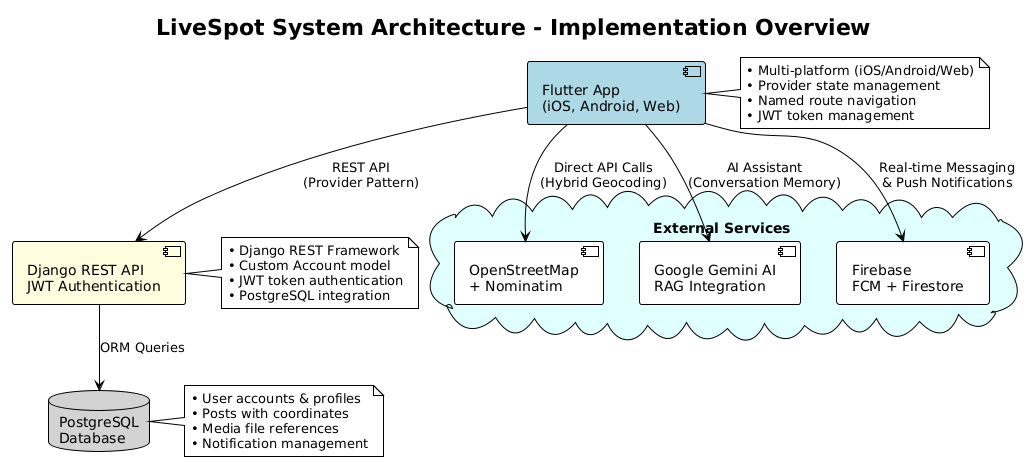
\includegraphics[width=0.9\textwidth]{figures/system_architecture}
    \caption{LiveSpot System Architecture Overview - Comprehensive view of the hybrid mobile-first architecture showing Flutter client, Django REST backend, PostgreSQL database, and external service integrations}
    \label{fig:system_architecture}
\end{figure}

Figure~\ref{fig:system_architecture} illustrates the complete system architecture encompassing all major components and their interactions. The architecture reflects the actual technology stack and service integrations implemented in the LiveSpot application, emphasizing the separation of concerns and scalable design patterns.

\subsection{Architectural Layers}

The architecture comprises three primary layers with clear separation of concerns:

\begin{itemize}
    \item \textbf{Presentation Layer:} Flutter cross-platform application with Provider state management and named routing
    \item \textbf{Business Logic Layer:} Django REST API backend with JWT authentication and service integrations
    \item \textbf{Data Layer:} PostgreSQL database with external service integrations (OSM, Gemini AI, Firebase)
\end{itemize}

\subsection{Architectural Patterns}

The system employs proven architectural patterns based on actual implementation:
\begin{itemize}
    \item \textbf{Provider Pattern:} Flutter state management with AccountProvider, PostsProvider, UserProfileProvider
    \item \textbf{REST API Architecture:} Django REST Framework with standardized endpoints and JWT authentication
    \item \textbf{Hybrid Service Integration:} OpenStreetMap primary with Google Geocoding fallback for cost optimization
    \item \textbf{RAG Integration:} Advanced AI assistant with contextual post retrieval and conversation memory
    \item \textbf{Multi-Platform Architecture:} Shared business logic across iOS, Android, and Web platforms
\end{itemize}

%%%%%%%%%%%%%%%%%%%%%%%%%%%%%%%%%%%%%%%%%%%%%%%%%%%%%%%%%%%%%%%%%%%%%%%%%%%%%%%%%%%
\section{Database Design}
\label{sec:database_design}

The database design follows PostgreSQL best practices with Django ORM integration, supporting the core functionality of location-based social networking with efficient relationships and data integrity.

\subsection{Entity Relationship Model}

The LiveSpot database architecture implements a comprehensive relational model designed to support real-time, location-based social networking functionality. The schema encompasses user management, content creation, social interactions, notification systems, and media storage with careful attention to performance optimization and data integrity.

\clearpage

\begin{figure}[p]
    \centering
    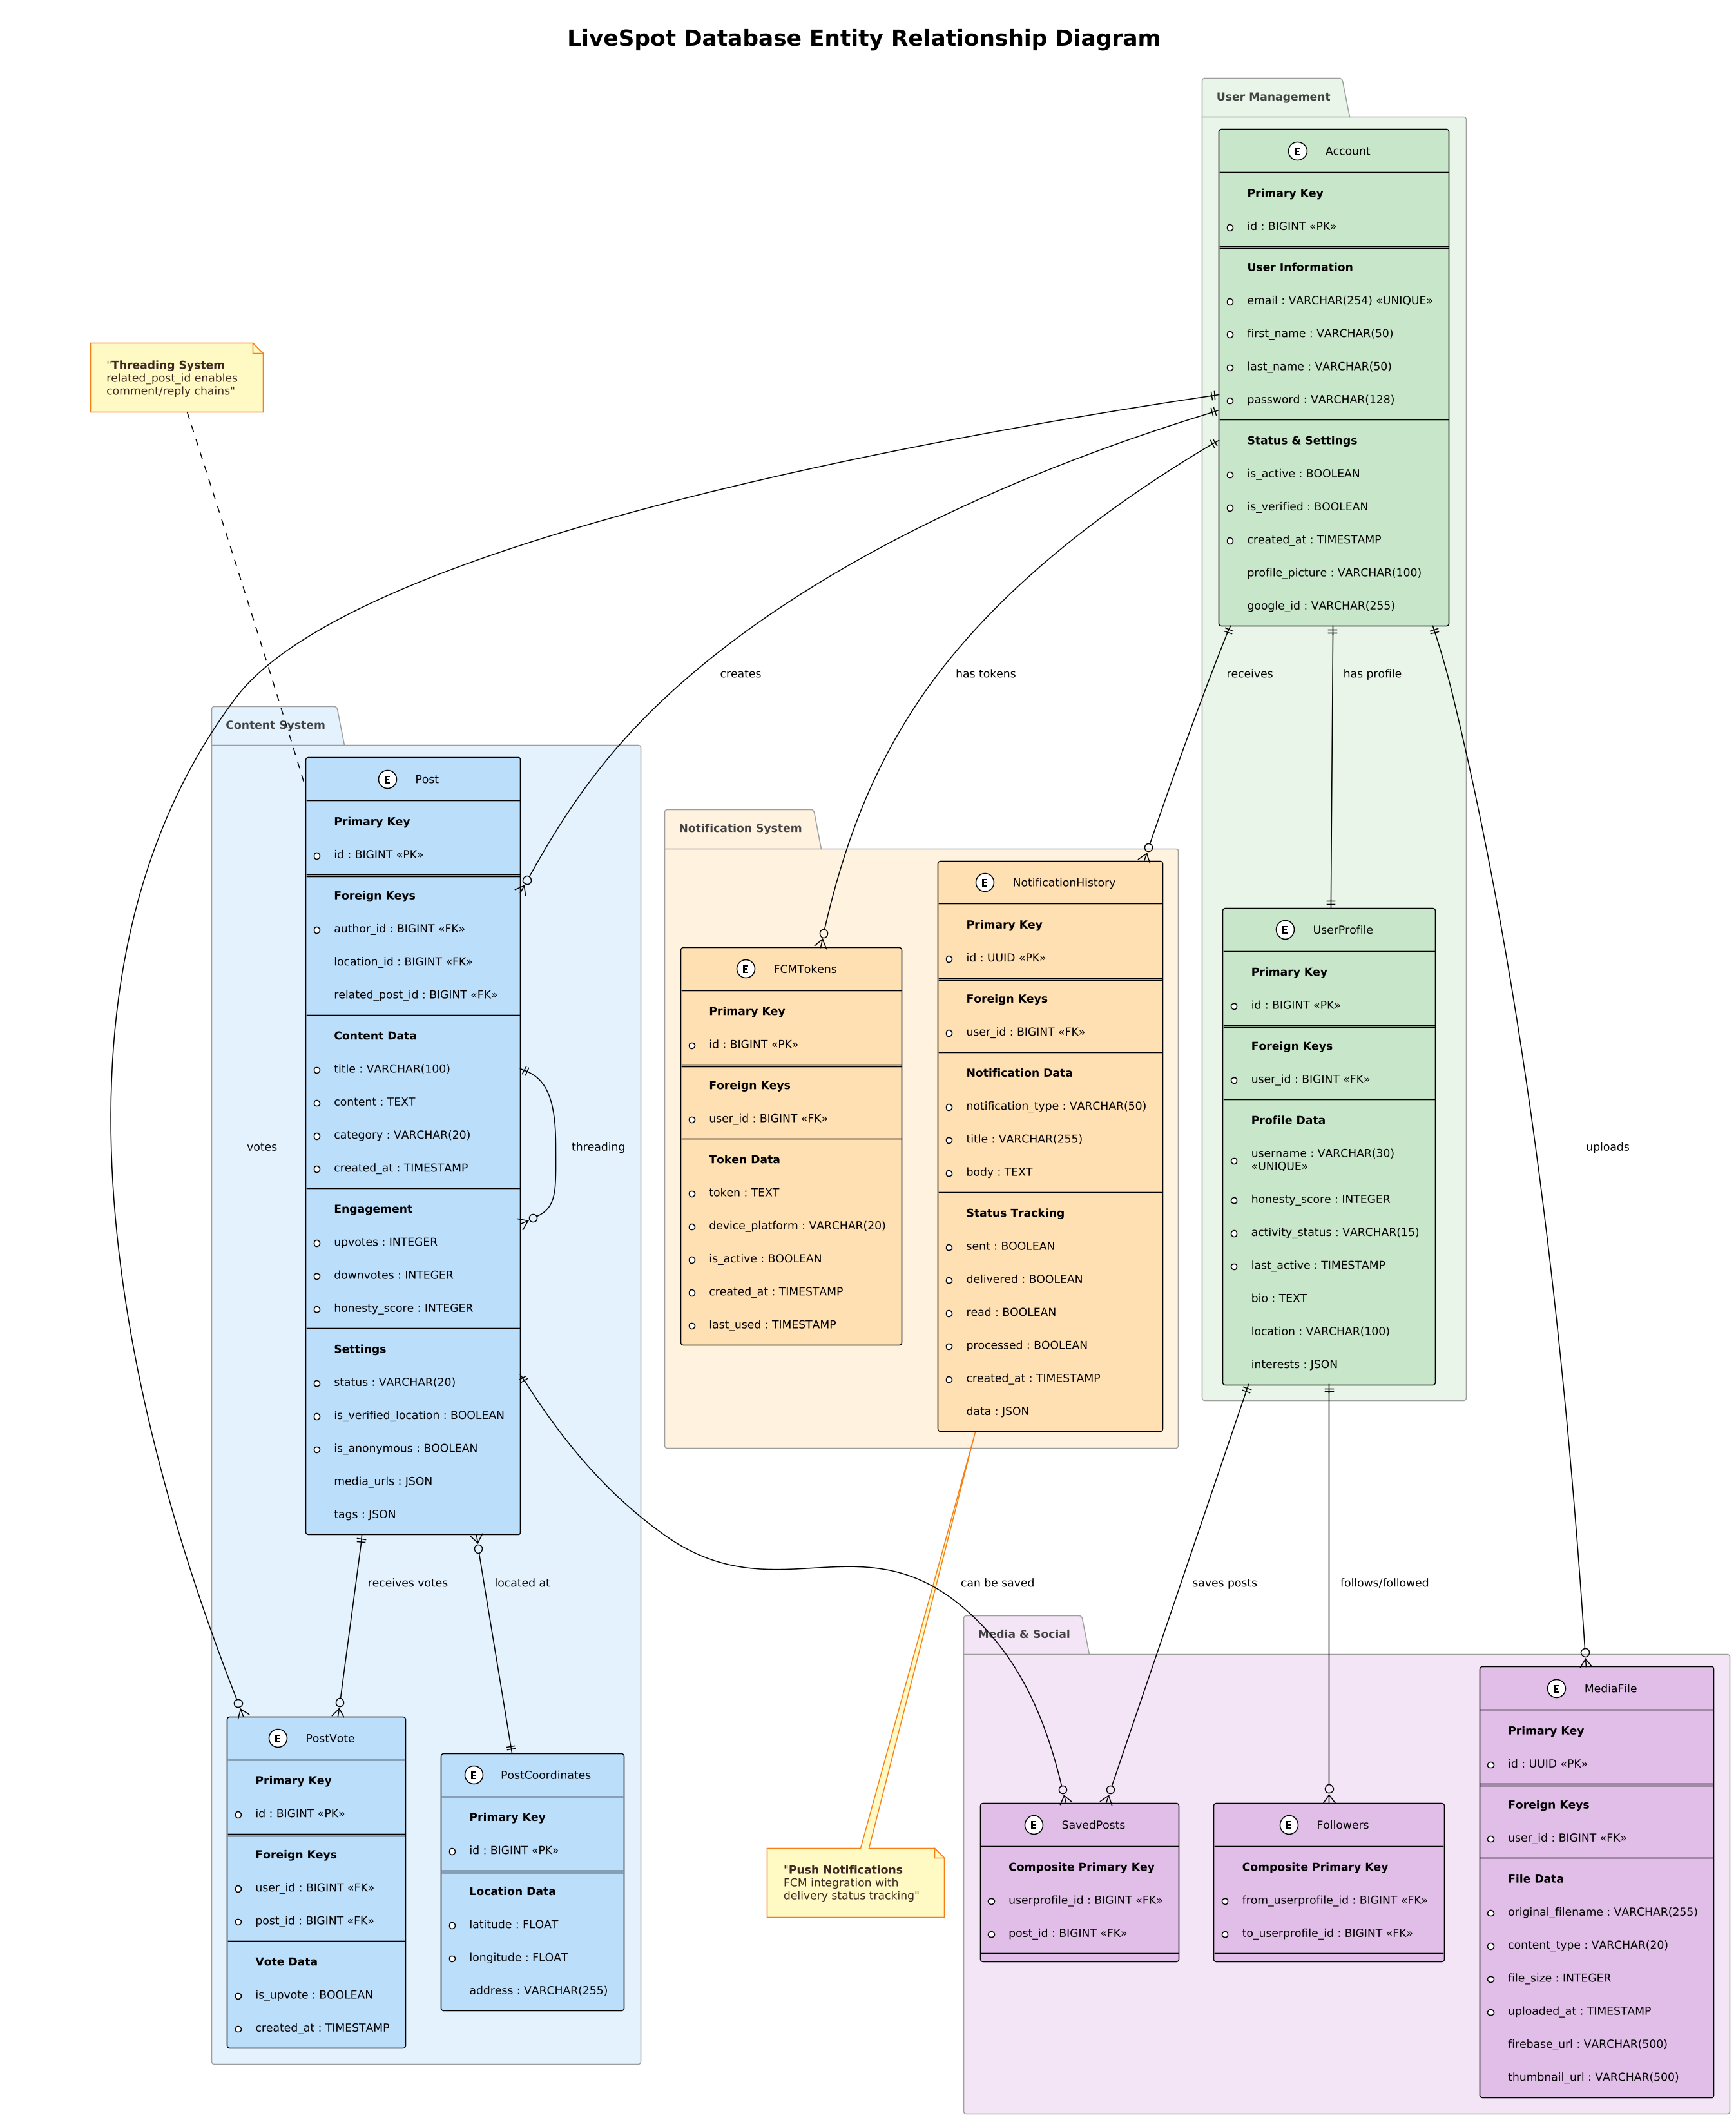
\includegraphics[width=\textwidth,height=0.9\textheight,keepaspectratio]{figures/database_erd}
    \caption{LiveSpot Database Entity Relationship Diagram - Complete schema showing all entities, relationships, and key attributes supporting location-verified social networking functionality}
    \label{fig:database_erd}
\end{figure}

\clearpage

The database schema illustrated in Figure~\ref{fig:database_erd} demonstrates the sophisticated relationship model underlying LiveSpot's functionality:

\textbf{Core User Management:}
\begin{itemize}
    \item \textbf{Account Entity:} Custom user model with authentication credentials, verification status, and account metadata
    \item \textbf{UserProfile Entity:} Extended user information including social features, activity tracking, and preference management
    \item \textbf{One-to-One Relationship:} Each account has exactly one profile, ensuring data consistency and optimal query performance
\end{itemize}

\textbf{Content and Location System:}
\begin{itemize}
    \item \textbf{Post Entity:} Central content model with threading support via \texttt{related\_post\_id} for comment-like functionality
    \item \textbf{PostCoordinates Entity:} Precise GPS location data with reverse-geocoded addresses for spatial queries
    \item \textbf{Threading Mechanism:} Self-referencing relationship enabling grouped discussions around specific events and locations
\end{itemize}

\textbf{Engagement and Social Features:}
\begin{itemize}
    \item \textbf{PostVote Entity:} User voting system with upvote/downvote functionality and duplicate prevention
    \item \textbf{SavedPosts Entity:} User bookmarking system with many-to-many relationship for content curation
    \item \textbf{Followers Entity:} Social networking capabilities enabling user-to-user following relationships
\end{itemize}

\textbf{Notification and Communication:}
\begin{itemize}
    \item \textbf{NotificationHistory Entity:} Comprehensive notification tracking with delivery status and metadata
    \item \textbf{FCMTokens Entity:} Push notification infrastructure supporting multiple devices per user
    \item \textbf{MediaFile Entity:} File storage management with Firebase integration for scalable media handling
\end{itemize}

\subsection{Firebase Integration}

Firebase services provide real-time messaging and push notification capabilities, complementing the PostgreSQL database for specific use cases that require instant delivery and offline synchronization.

% TODO: Add Firebase Data Model Diagram
% Figure~\ref{fig:firebase_schema} shows Firestore collections and document structure
\clearpage
%%%%%%%%%%%%%%%%%%%%%%%%%%%%%%%%%%%%%%%%%%%%%%%%%%%%%%%%%%%%%%%%%%%%%%%%%%%%%%%%%%%
\section{UML Sequence Diagrams}
\label{sec:sequence_diagrams}

The following sequence diagrams illustrate key user interaction flows and system behavior for critical LiveSpot functionality. Each diagram demonstrates the complete workflow for essential application features.

\subsection{User Authentication Flow}

The authentication system implements a secure JWT-based workflow with integrated FCM token registration for push notifications.

\begin{figure}[h!]
    \centering
    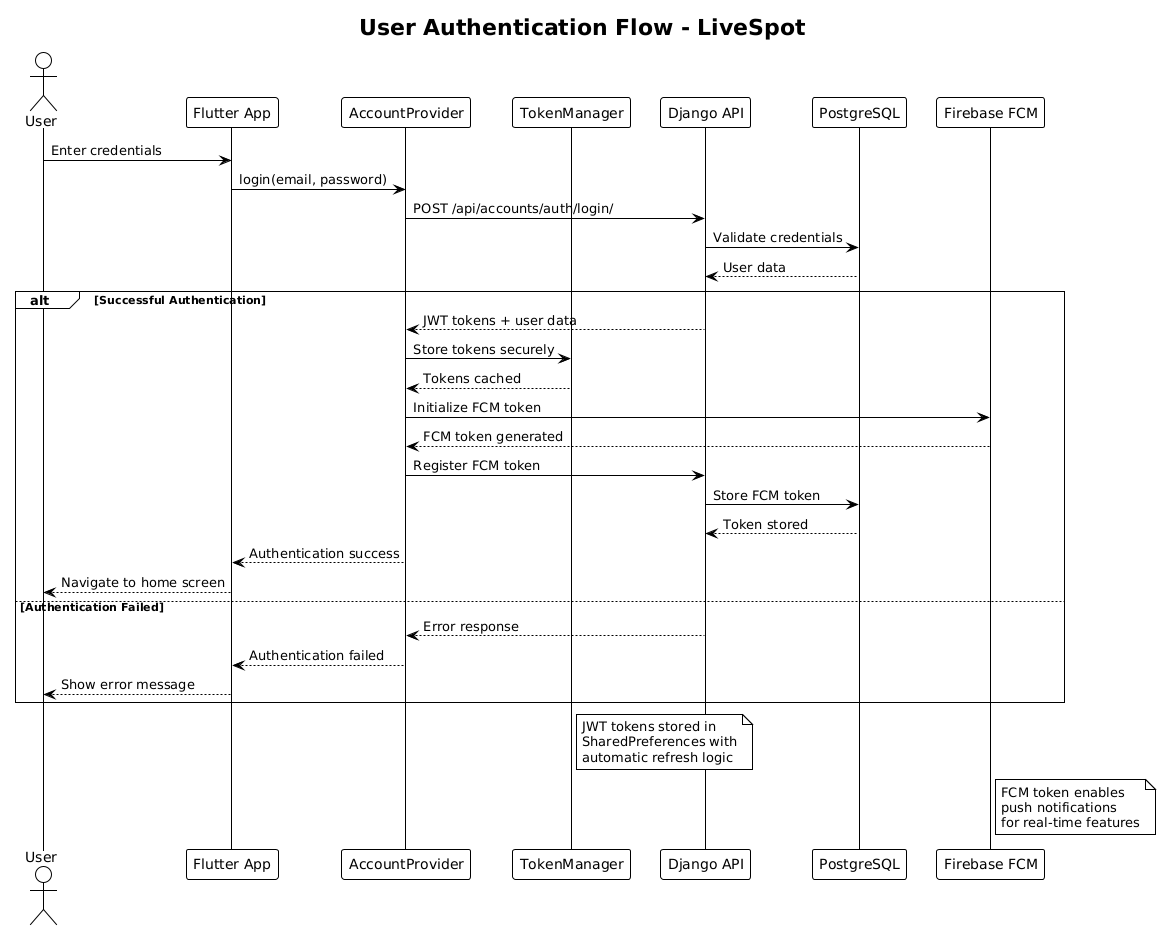
\includegraphics[width=0.95\textwidth]{figures/authentication_sequence}
    \caption{User Authentication Sequence Diagram - Complete JWT-based login flow showing credential validation, token generation, FCM registration, and session establishment}
    \label{fig:auth_sequence}
\end{figure}

Figure~\ref{fig:auth_sequence} demonstrates the comprehensive authentication workflow from initial user credential entry through successful JWT token storage and FCM token registration for push notifications. The sequence ensures secure user access while enabling real-time notification capabilities.
\clearpage
\subsection{Post Creation and Threading Flow}

The post creation system supports both standalone posts and threaded discussions with location verification and temporal constraints.

\begin{figure}[h!]
    \centering
    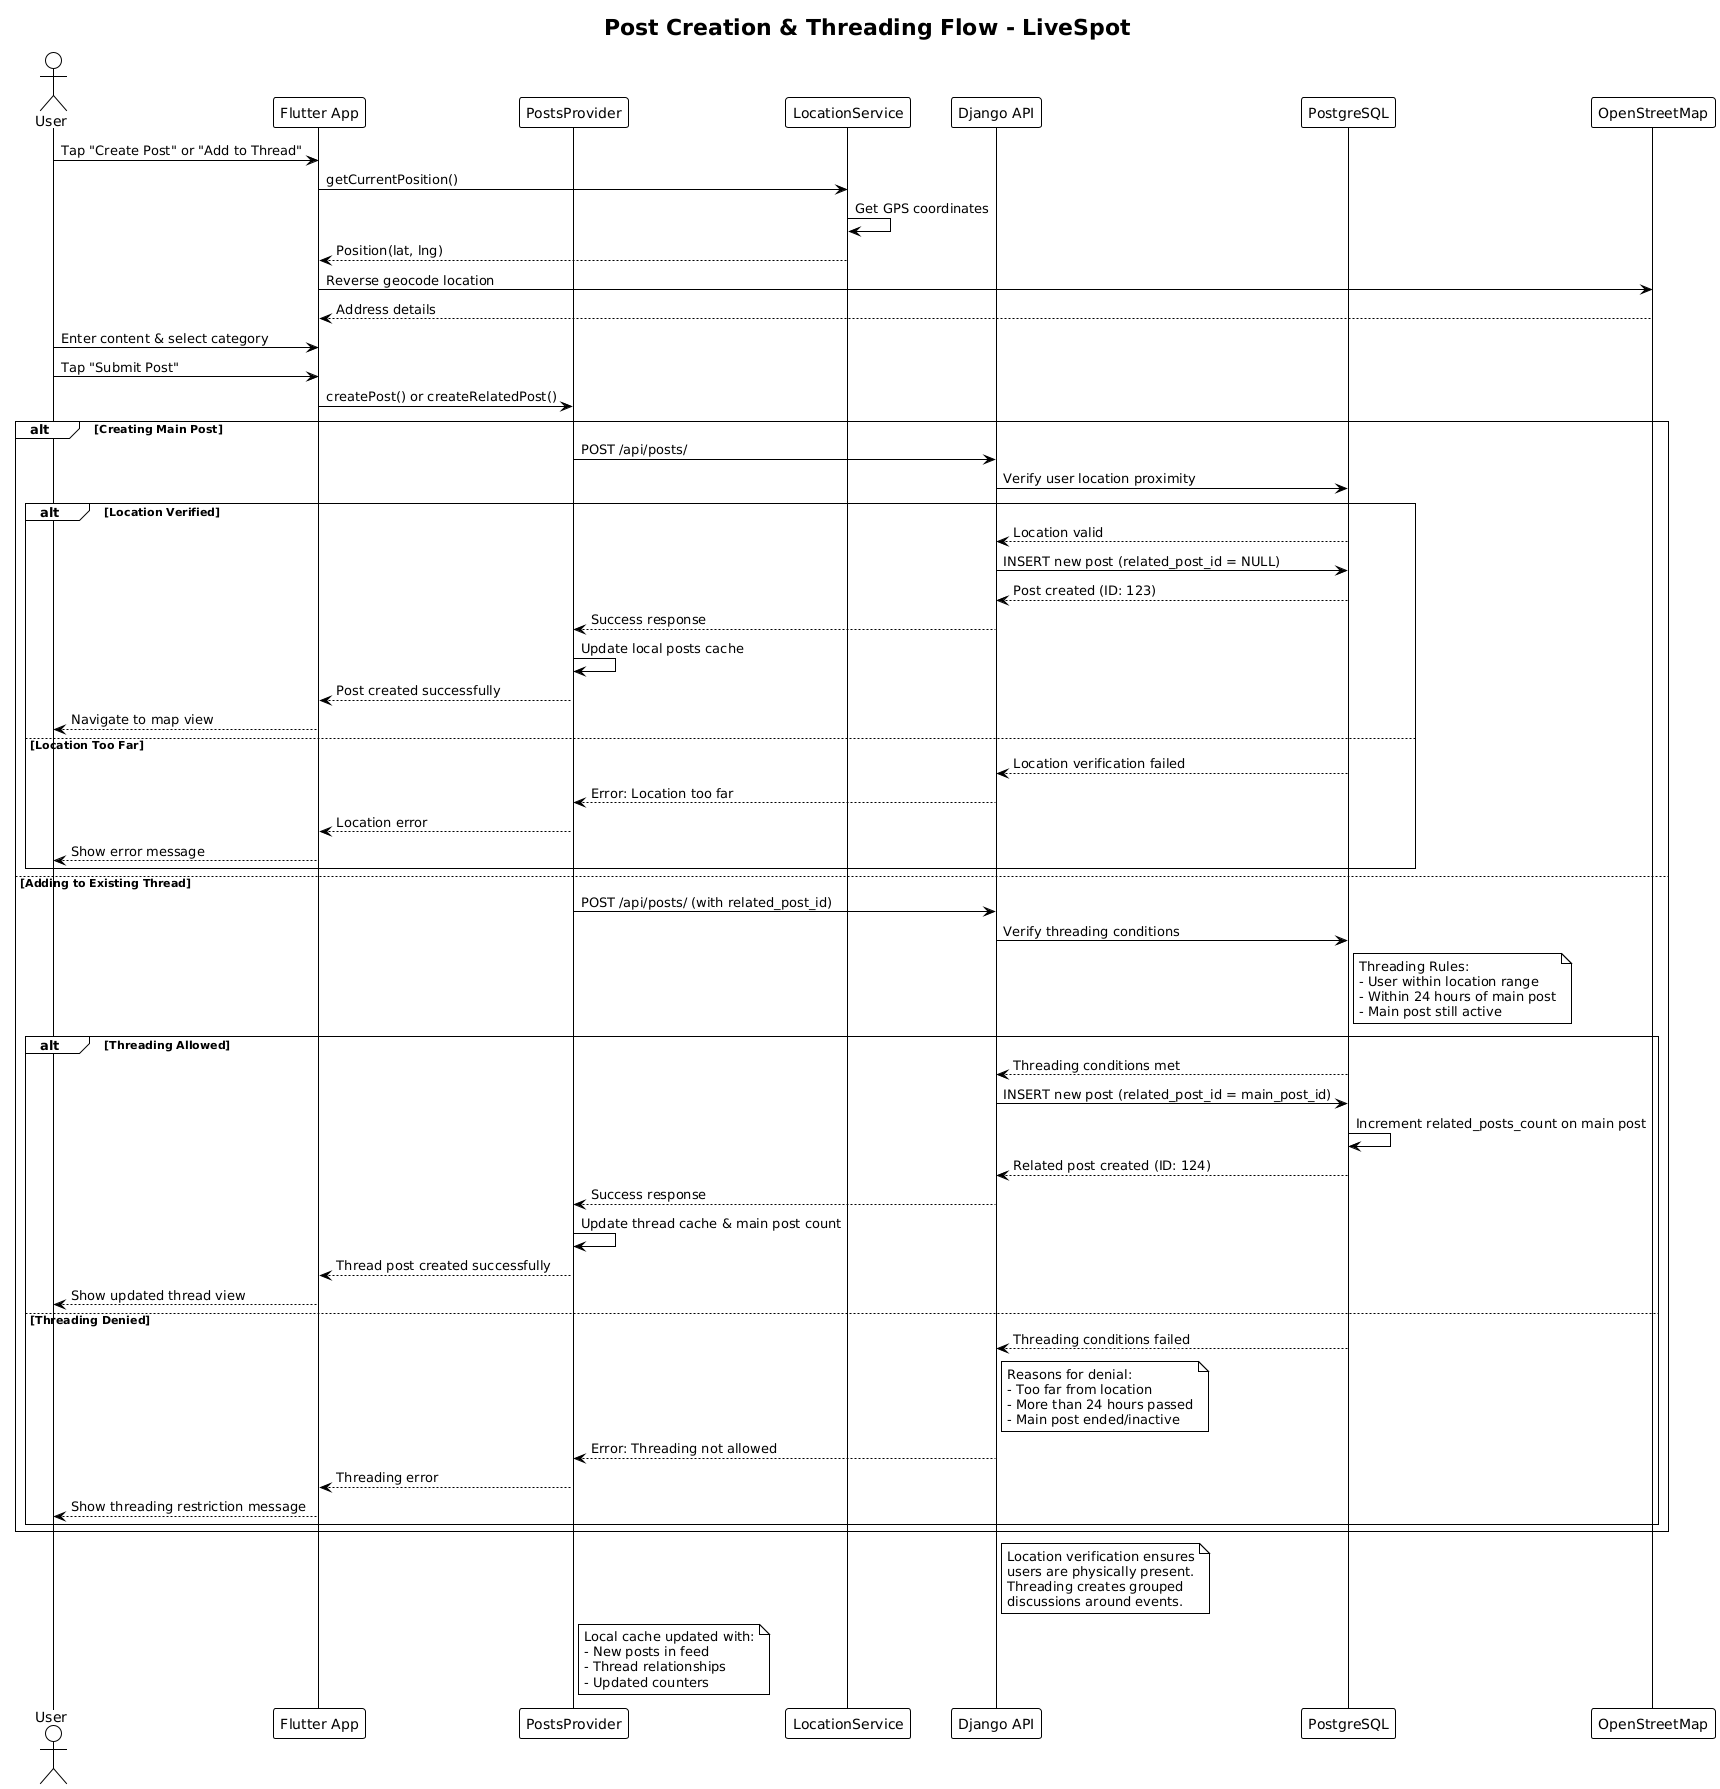
\includegraphics[width=\textwidth,height=0.75\textheight,keepaspectratio]{figures/post_creation_sequence}
    \caption{Post Creation and Threading Sequence Diagram}
    \label{fig:post_creation_sequence}
\end{figure}

Figure~\ref{fig:post_creation_sequence} illustrates the sophisticated post creation process encompassing location verification, reverse geocoding, threading decision logic, and database persistence. The diagram highlights the system's ability to create both main posts and related threaded posts with appropriate validation mechanisms.
\clearpage
\subsection{Real-time Messaging Flow}

The messaging architecture combines Firebase Firestore for real-time delivery with FCM for offline push notifications.

\begin{figure}[h!]
    \centering
    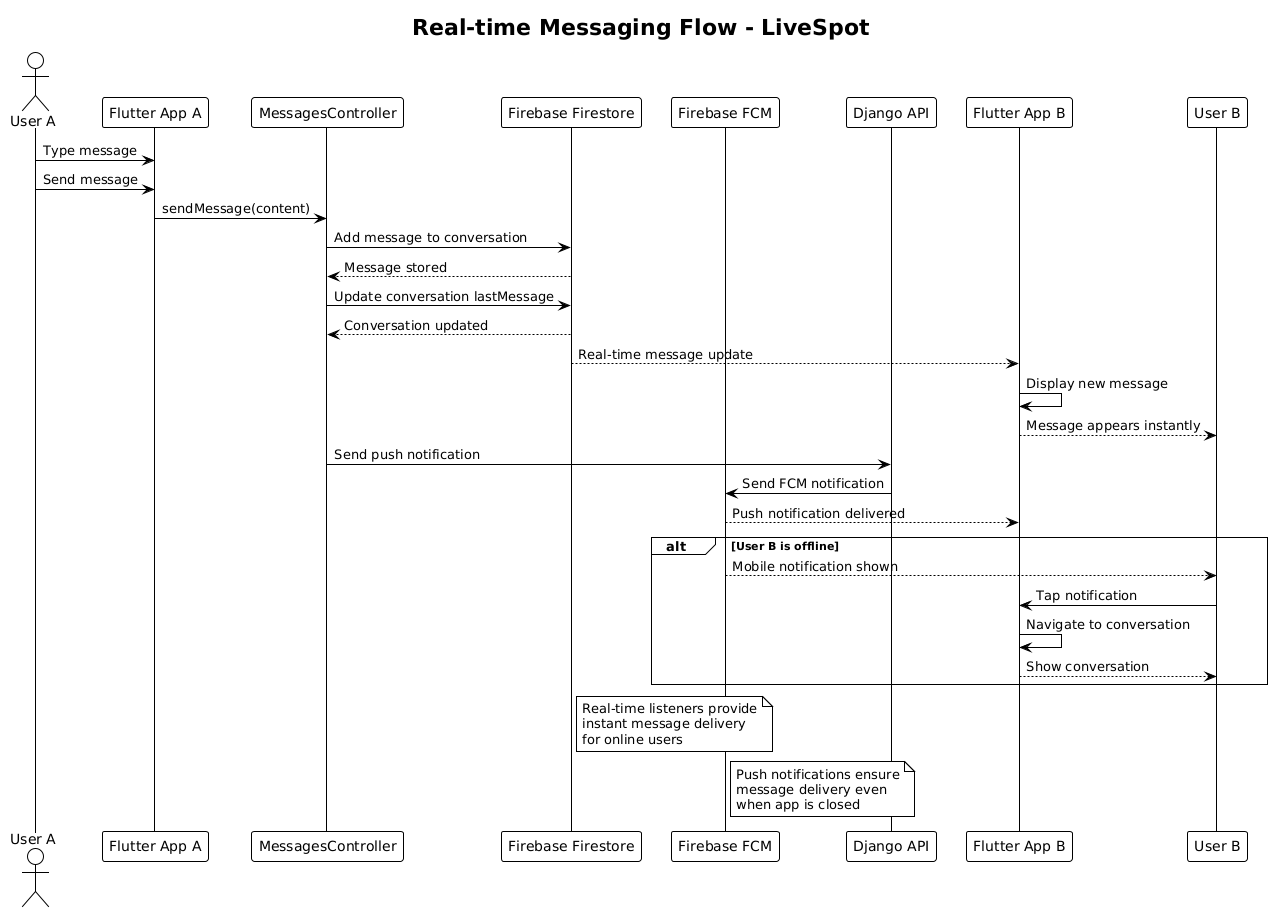
\includegraphics[width=0.95\textwidth]{figures/messaging_sequence}
    \caption{Real-time Messaging Sequence Diagram - Hybrid messaging architecture combining Firebase Firestore real-time synchronization with FCM push notifications for comprehensive communication coverage}
    \label{fig:messaging_sequence}
\end{figure}

Figure~\ref{fig:messaging_sequence} shows the hybrid messaging architecture that ensures reliable message delivery across different user states (online, offline, background). The system leverages Firebase Firestore for instant real-time synchronization and FCM for push notifications when users are not actively using the application.

%%%%%%%%%%%%%%%%%%%%%%%%%%%%%%%%%%%%%%%%%%%%%%%%%%%%%%%%%%%%%%%%%%%%%%%%%%%%%%%%%%%
\section{API Design and Integration}
\label{sec:api_design}

\subsection{RESTful API Architecture}

The LiveSpot API architecture implements a clean Django REST Framework backend with organized endpoint structure, JWT authentication, and external service integrations. The architecture supports cross-platform Flutter clients through standardized JSON communication patterns.

\begin{figure}[h!]
    \centering
    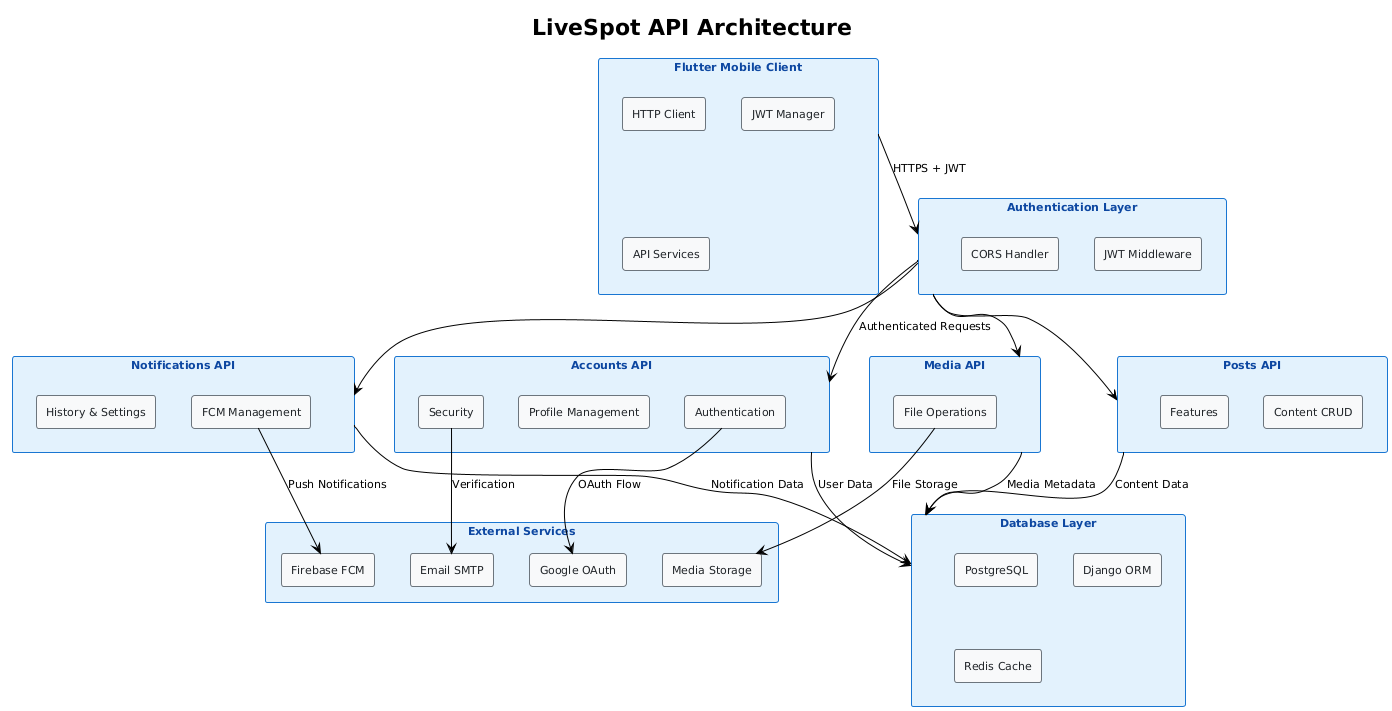
\includegraphics[width=0.8\textwidth]{figures/api_architecture}
    \caption{LiveSpot REST API Architecture - Vertical layout showing layered architecture from Flutter client through authentication middleware to organized API endpoints with external service integrations}
    \label{fig:api_architecture}
\end{figure}

Figure~\ref{fig:api_architecture} illustrates the vertical API architecture with clear separation between client, authentication, API endpoints, external services, and database layers. The design follows REST principles with organized endpoint grouping across four main domains: Accounts, Posts, Notifications, and Media APIs.

The architecture employs JWT middleware for secure authentication, CORS handling for cross-platform access, and seamless integration with external services including Firebase for notifications, Google OAuth for authentication, and cloud storage for media files. This layered approach ensures scalable, maintainable API design that supports the Flutter mobile application's requirements.

\subsection{External Service Integration}

Integration with third-party services expands functionality and improves user experience while maintaining cost-effectiveness and reliability through strategic service selection and hybrid approaches.

\begin{figure}[h!]
    \centering
    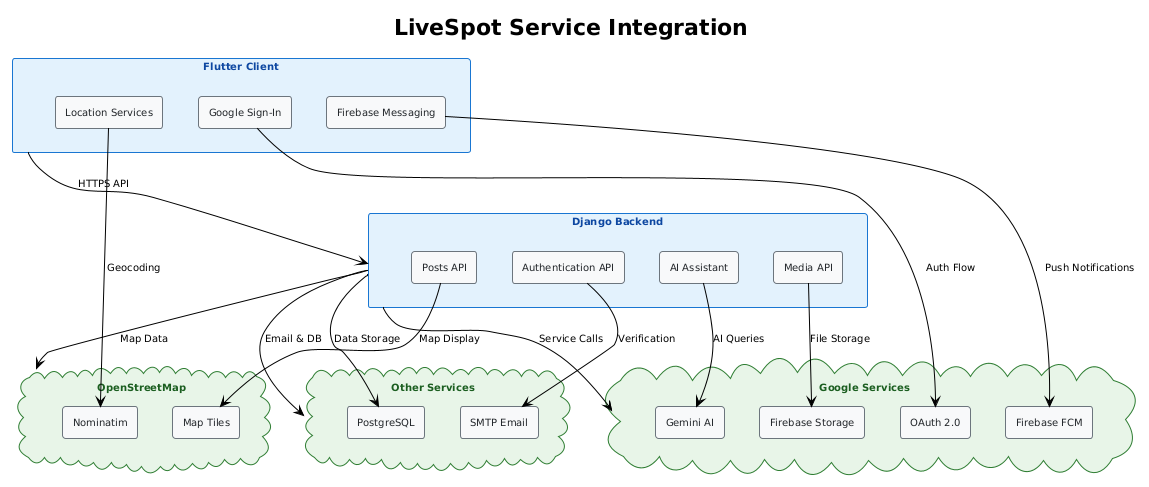
\includegraphics[width=0.7\textwidth]{figures/service_integrations}
    \caption{Service Integration Architecture - Simplified vertical view of external service connections showing the layered integration approach from Flutter client through Django backend to various cloud services}
    \label{fig:service_integrations}
\end{figure}

Figure~\ref{fig:service_integrations} illustrates LiveSpot's streamlined service integration architecture with a clear vertical flow from client to external services. The design emphasizes the strategic layering of services for optimal cost-effectiveness and reliability.

The integration follows a hybrid approach: free services like OpenStreetMap and Nominatim for primary functionality, with Google services providing enhanced features and reliable fallbacks. Firebase services handle real-time capabilities, while traditional infrastructure services like PostgreSQL and SMTP ensure robust data persistence and communication.

%%%%%%%%%%%%%%%%%%%%%%%%%%%%%%%%%%%%%%%%%%%%%%%%%%%%%%%%%%%%%%%%%%%%%%%%%%%%%%%%%%%
\section{Security Architecture}
\label{sec:security_architecture}

\subsection{Authentication and Authorization}

The system implements a JWT-based authentication architecture with hybrid fallback mechanisms, providing secure user access without relying on external authentication providers.

\begin{figure}[h!]
    \centering
    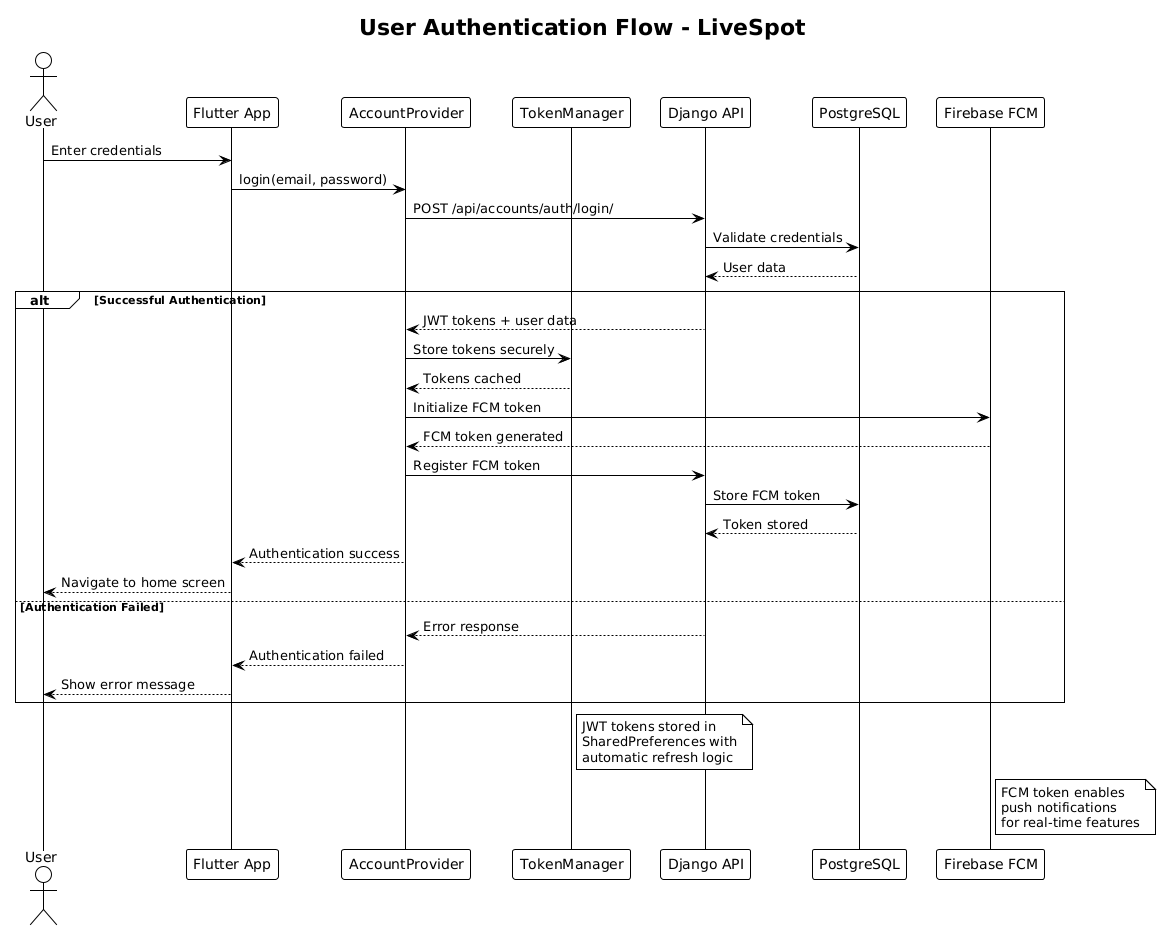
\includegraphics[width=0.95\textwidth]{figures/authentication_sequence}
    \caption{JWT Authentication Sequence Diagram - Complete authentication flow showing JWT token lifecycle, Google OAuth integration, and FCM token registration for secure user access and push notifications}
    \label{fig:auth_flow}
\end{figure}

Figure~\ref{fig:auth_flow} illustrates the comprehensive authentication flow including JWT token generation, Google OAuth integration, and Firebase Cloud Messaging token registration. The sequence demonstrates the secure handshake between Flutter client and Django backend, ensuring authenticated user sessions and push notification capabilities.
\clearpage
\subsection{Security Layers and Protection Mechanisms}

LiveSpot implements a comprehensive multi-layered security architecture that protects user data and system integrity at every level of the application stack.

\begin{figure}[h!]
    \centering
    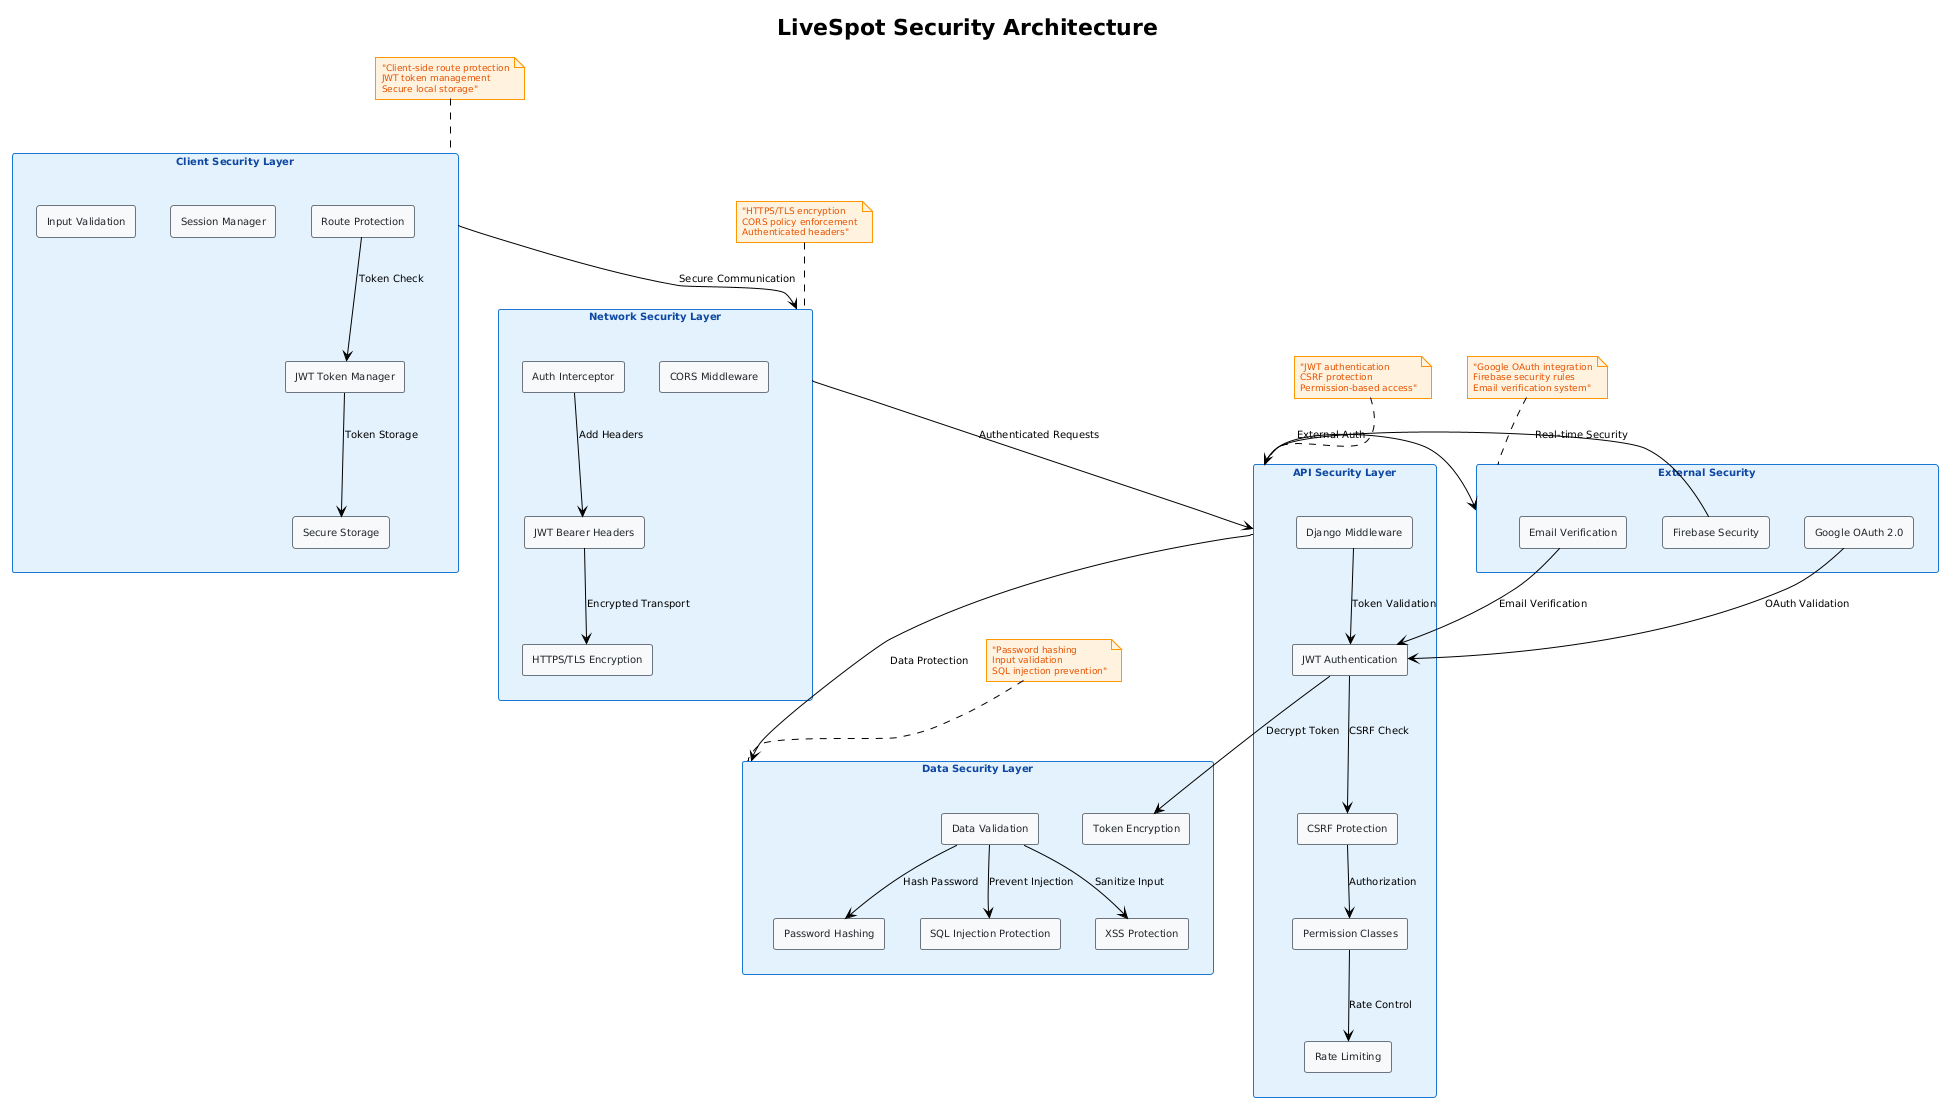
\includegraphics[width=0.8\textwidth]{figures/security_architecture}
    \caption{Security Architecture - Multi-layered security implementation showing client-side protection, network security, API authentication, data encryption, and external service security integration}
    \label{fig:security_architecture}
\end{figure}

Figure~\ref{fig:security_architecture} demonstrates the comprehensive security framework implemented across all system layers. The architecture incorporates client-side route protection, JWT token management with automatic refresh, secure network communications, API-level authentication and authorization, data encryption and validation, and integration with secure external services including Google OAuth and Firebase security features.

%%%%%%%%%%%%%%%%%%%%%%%%%%%%%%%%%%%%%%%%%%%%%%%%%%%%%%%%%%%%%%%%%%%%%%%%%%%%%%%%%%%
\section{Technology Stack}
\label{sec:technology_stack}

\subsection{Frontend Technology Stack}

Rationale for technology selections supporting cross-platform development.

\begin{table}[h!]
    \centering
    \caption{Frontend Technology Stack}
    \label{tab:frontend_stack}
    \begin{tabular}{lll}     
        \toprule
        Category & Technology & Justification \\
        \midrule
        Framework & Flutter & Cross-platform, native performance \\
        State Management & Provider & Simple, efficient state handling \\
        Navigation & Named Routes & Declarative routing system \\
        HTTP Client & Dio & Advanced HTTP features \\
        Local Storage & SharedPreferences & Simple key-value storage \\
        Authentication & Custom JWT & Secure token management \\
        Maps & OpenStreetMap & Free, reliable mapping service \\
        Geocoding & Nominatim + Google & Hybrid geocoding approach \\
        AI Integration & Google Gemini & Advanced conversational AI \\
        \bottomrule
    \end{tabular}
\end{table}
\clearpage
\subsection{Backend Technology Stack}

Server-side technology choices supporting scalability and maintainability.

\begin{table}[h!]
    \centering
    \caption{Backend Technology Stack}
    \label{tab:backend_stack}
    \begin{tabular}{lll}     
        \toprule
        Category & Technology & Justification \\
        \midrule
        Framework & Django REST Framework & Robust API development \\
        Database & PostgreSQL & ACID compliance, performance \\
        Authentication & JWT Tokens & Stateless authentication \\
        Session Management & Custom SessionManager & Session lifecycle control \\
        File Storage & Firebase Storage & Scalable media storage \\
        Push Notifications & Firebase FCM & Reliable message delivery \\
        API Documentation & Django REST Browsable & Interactive API docs \\
        \bottomrule
    \end{tabular}
\end{table}

%%%%%%%%%%%%%%%%%%%%%%%%%%%%%%%%%%%%%%%%%%%%%%%%%%%%%%%%%%%%%%%%%%%%%%%%%%%%%%%%%%%
\section{Summary}

The LiveSpot system design presents a comprehensive, scalable architecture that effectively addresses the requirements for real-time, location-based social networking. The layered architecture with clear separation of concerns enables maintainable code, while the cloud-native approach ensures scalability and reliability. 

The integration of multiple technologies—Flutter for cross-platform development, OpenStreetMap for cost-effective mapping, Firebase for real-time capabilities, Django for robust backend services, and Google Gemini AI for intelligent features—creates a cohesive system capable of supporting large-scale social interactions while maintaining performance and security standards.

The design emphasizes user experience through responsive interfaces, accurate location services, and AI-powered assistance, while maintaining technical excellence through proper architectural patterns, comprehensive security measures, and scalable infrastructure. The detailed architectural diagrams, sequence flows, and component relationships provide a complete blueprint for implementation and future system evolution.

This foundation provides the necessary technical capability to support the application's core mission of creating trustworthy, location-based community reporting and social networking, with built-in scalability to accommodate growth and feature expansion while maintaining cost-effectiveness through the use of open-source and free services where appropriate.

    \chapter{Results}\label{ch:results}

This chapter presents the comprehensive implementation results of the LiveSpot application, a cross-platform location-based social networking platform. The results demonstrate the successful development of a feature-rich application that addresses real-world challenges in information verification, community engagement, and location-based content sharing through innovative technological solutions and user-centric design principles.

\section{Application Implementation}\label{sec:app_implementation}

This section presents the complete implementation of the LiveSpot application, demonstrating the successful development of a cross-platform, location-based social networking platform. The implementation showcases the integration of real-time messaging, location verification, community-driven content management, and intelligent AI-powered features across mobile and web platforms.

\subsection{UI/UX Design}\label{subsec:ui_ux_design}

The LiveSpot application implements a comprehensive UI/UX design that prioritizes user accessibility, cross-platform consistency, and intuitive navigation. The interface design follows Material Design principles through Flutter's cross-platform framework, ensuring a cohesive user experience across Android, iOS, and web platforms.

\subsubsection{Cross-Platform Design}\label{subsubsec:cross_platform_design}

The application maintains visual and functional consistency across all platforms through Flutter's unified codebase. The design system employs consistent color schemes, typography, and interaction patterns that adapt appropriately to platform-specific conventions while preserving the application's unique identity.

\textbf{Theme Support and Visual Modes:}
LiveSpot implements comprehensive theming support with both light and dark mode options seamlessly available across all platforms (Android, iOS, and web). The application intelligently detects system preferences while providing users the flexibility to manually override theme settings according to their preferences. Throughout the development and testing phases, the Android platform exemplifies the elegant dark theme implementation with rich contrast and visual depth, while the web platform showcases the clean and accessible light mode interface. Both visual modes maintain consistent branding elements, typography hierarchy, and accessibility standards, ensuring optimal user experience regardless of preferred visual setting or platform choice.

\subsubsection{Authentication Interface}\label{subsubsec:auth_interface}

The authentication system provides a seamless user onboarding experience with comprehensive registration, login, and password recovery workflows. The interface design strategically prioritizes user trust establishment through transparent privacy explanations and clear communication of data usage policies.

\paragraph{Account Creation and Verification Flow}
The account registration process provides a complete user onboarding experience from initial welcome screen through account creation and email verification. The mobile implementation demonstrates the elegant dark theme with clear step-by-step guidance.

\textbf{Mobile Interface (Android):}
\begin{figure}[!htbp]
    \centering
    \subfigure[Welcome Screen]{
        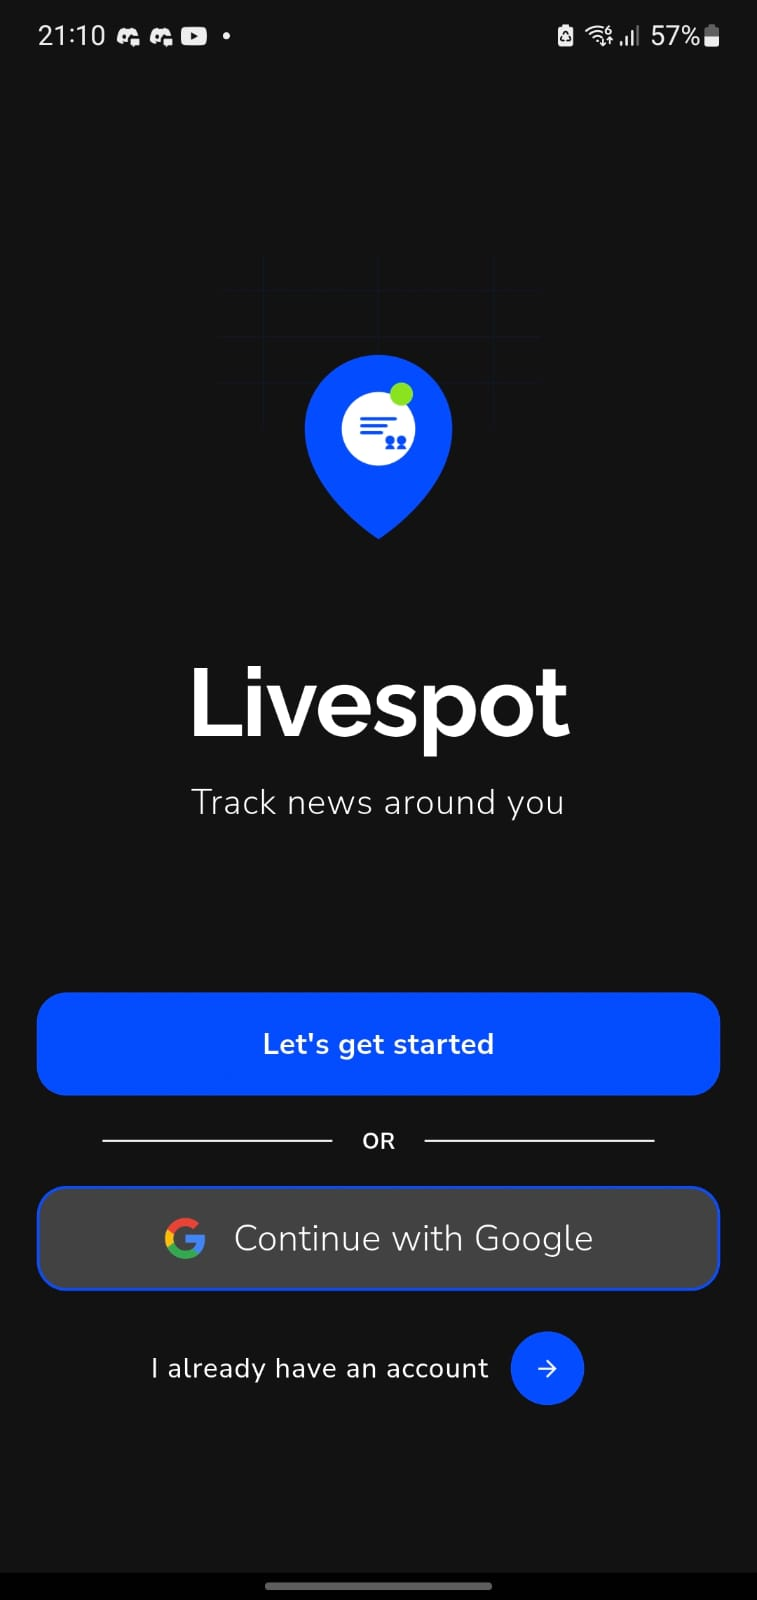
\includegraphics[width=0.32\textwidth]{figures/ui/get_started_android.jpeg}
    }%
    \subfigure[Create Account]{
        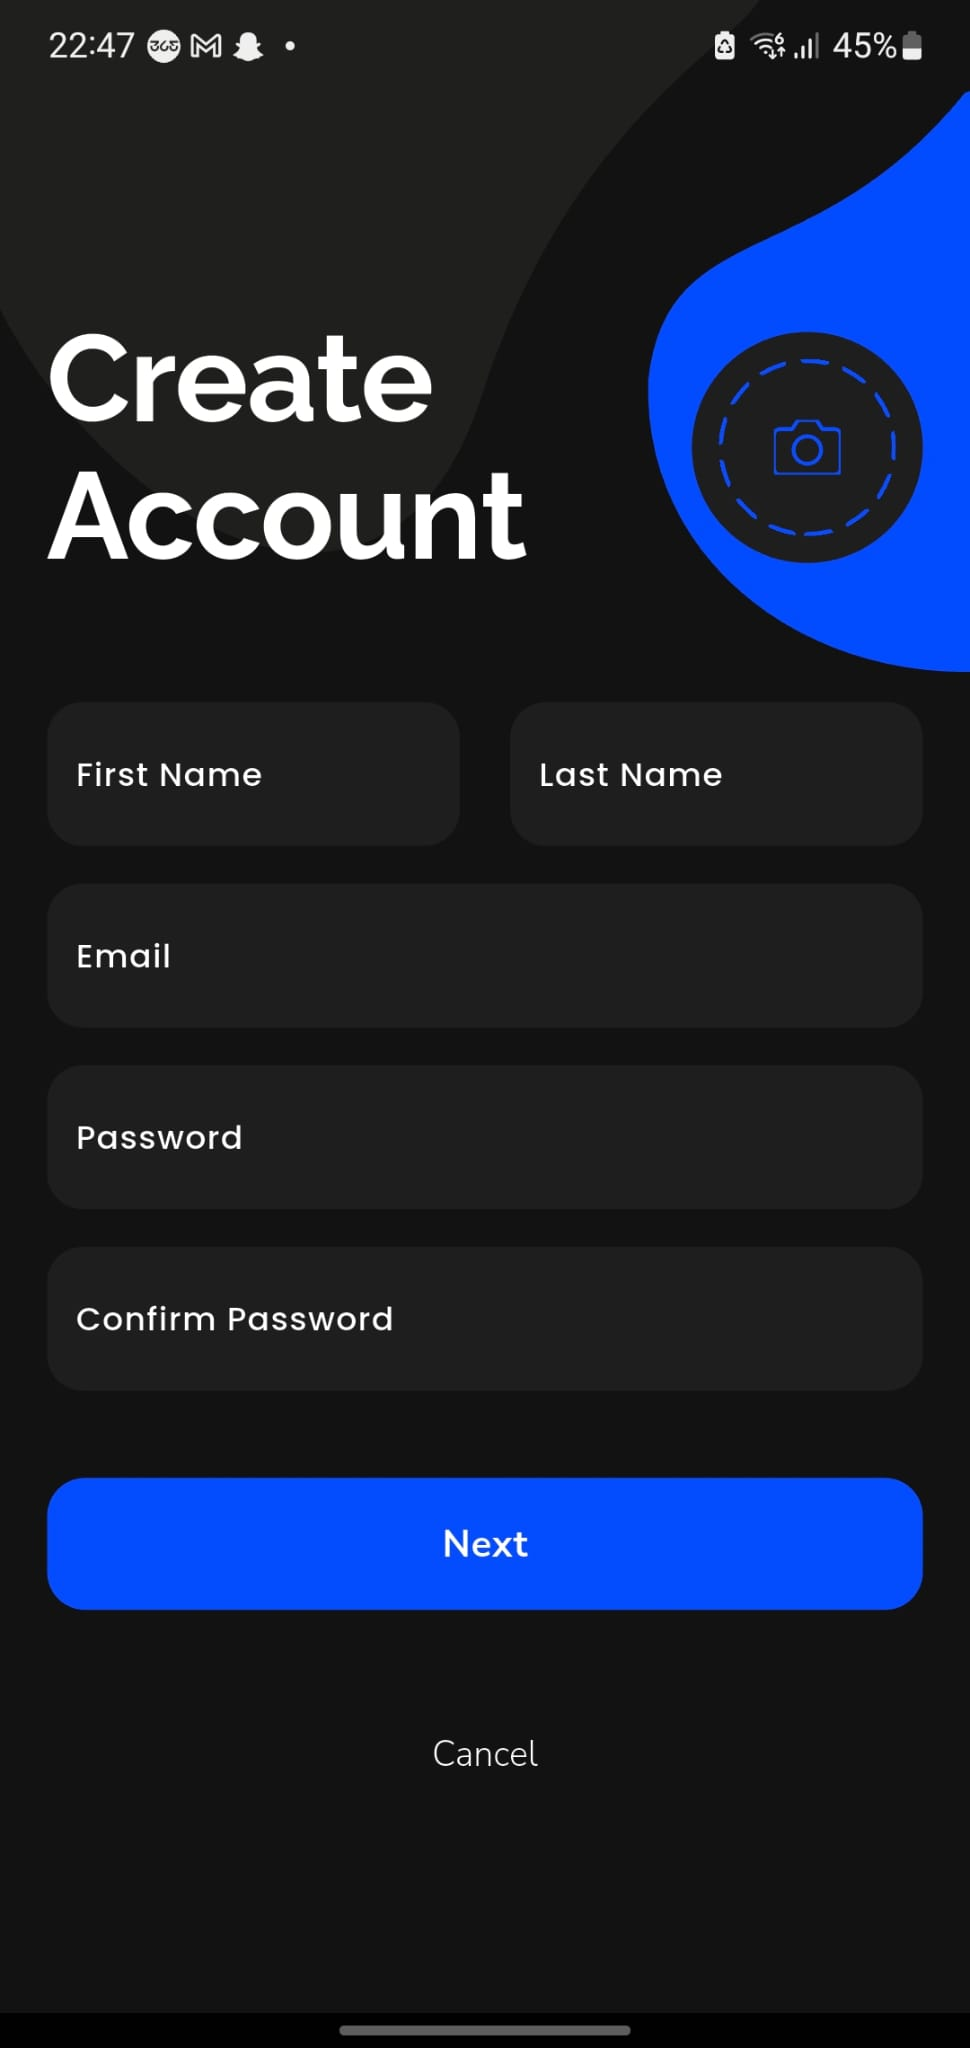
\includegraphics[width=0.32\textwidth]{figures/ui/create_account_android.jpeg}
    }%
    \subfigure[Email Verification]{
        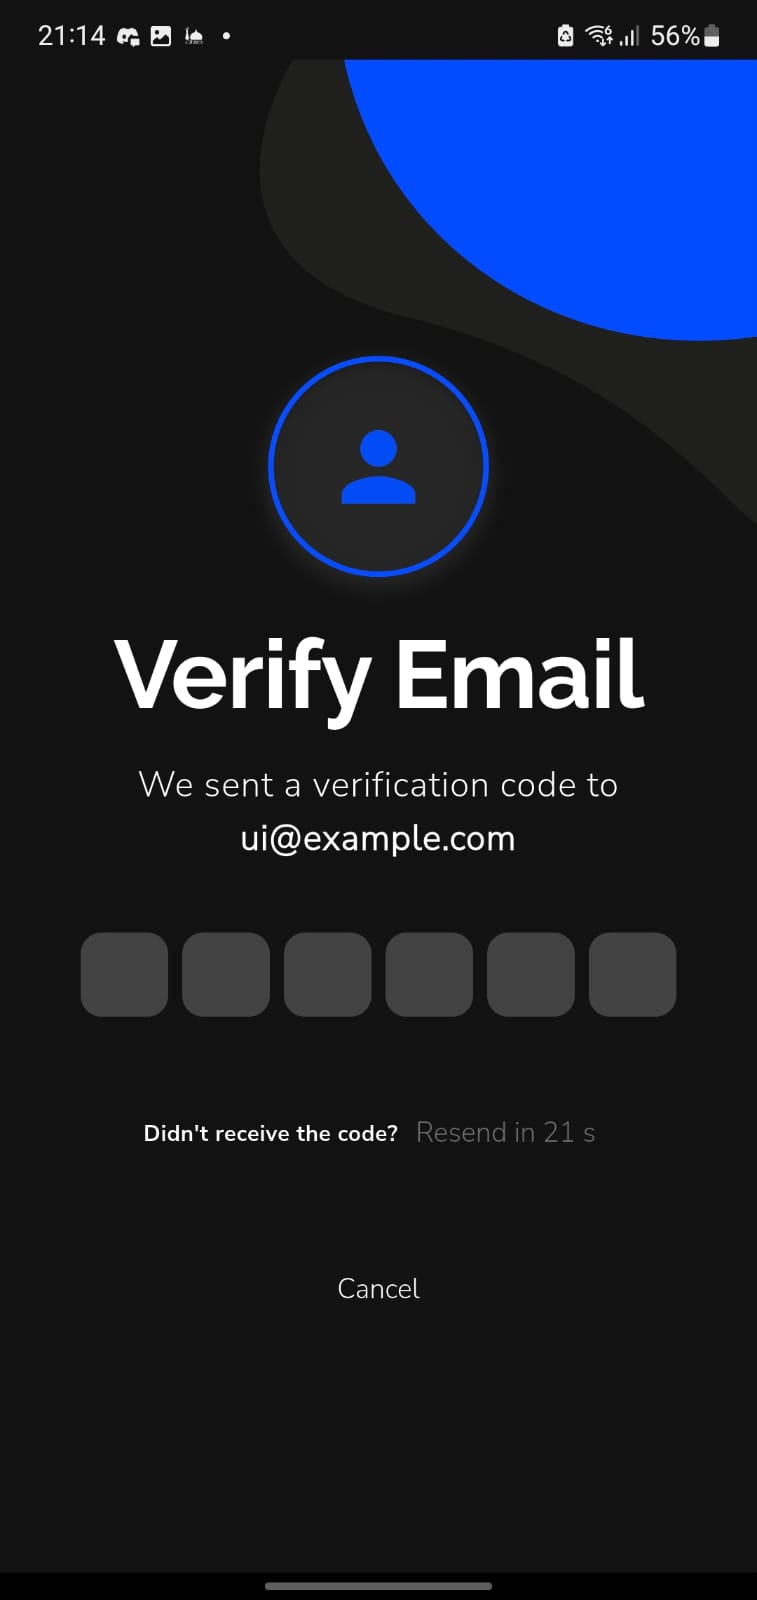
\includegraphics[width=0.32\textwidth]{figures/ui/verify_email_signup_android.jpeg}
    }
    \caption{Account Creation Flow on Android---Dark Theme Implementation}\label{fig:android_account_creation}
\end{figure}

The account creation process implements comprehensive security measures and multiple authentication options to ensure user convenience while maintaining platform security:

\textbf{Authentication Options and Security Features:}
\begin{itemize}
    \item \textbf{Multiple Registration Methods:} Users can create accounts using either traditional email/password combinations or streamlined Google OAuth integration, providing flexibility based on user preferences
    \item \textbf{Strong Password Requirements:} The system enforces robust password policies including minimum length (8 characters), uppercase and lowercase letters, numbers, and special characters with real-time strength indicators
    \item \textbf{Email Validation:} Comprehensive email verification includes format validation, domain verification, and automated confirmation emails to ensure authentic user registration
    \item \textbf{Google OAuth Integration:} Seamless social authentication reduces registration friction while leveraging Google's secure authentication infrastructure
    \item \textbf{Real-time Form Validation:} Instant feedback on form fields prevents common registration errors and guides users toward successful account creation
    \item \textbf{Privacy Compliance:} Clear privacy policy presentation and consent mechanisms ensure GDPR and data protection compliance during registration
\end{itemize}

\textbf{Web Interface:}
The web implementation showcases the clean light theme with responsive design that adapts beautifully to desktop and tablet screens.

\begin{figure}[!htbp]
    \centering
    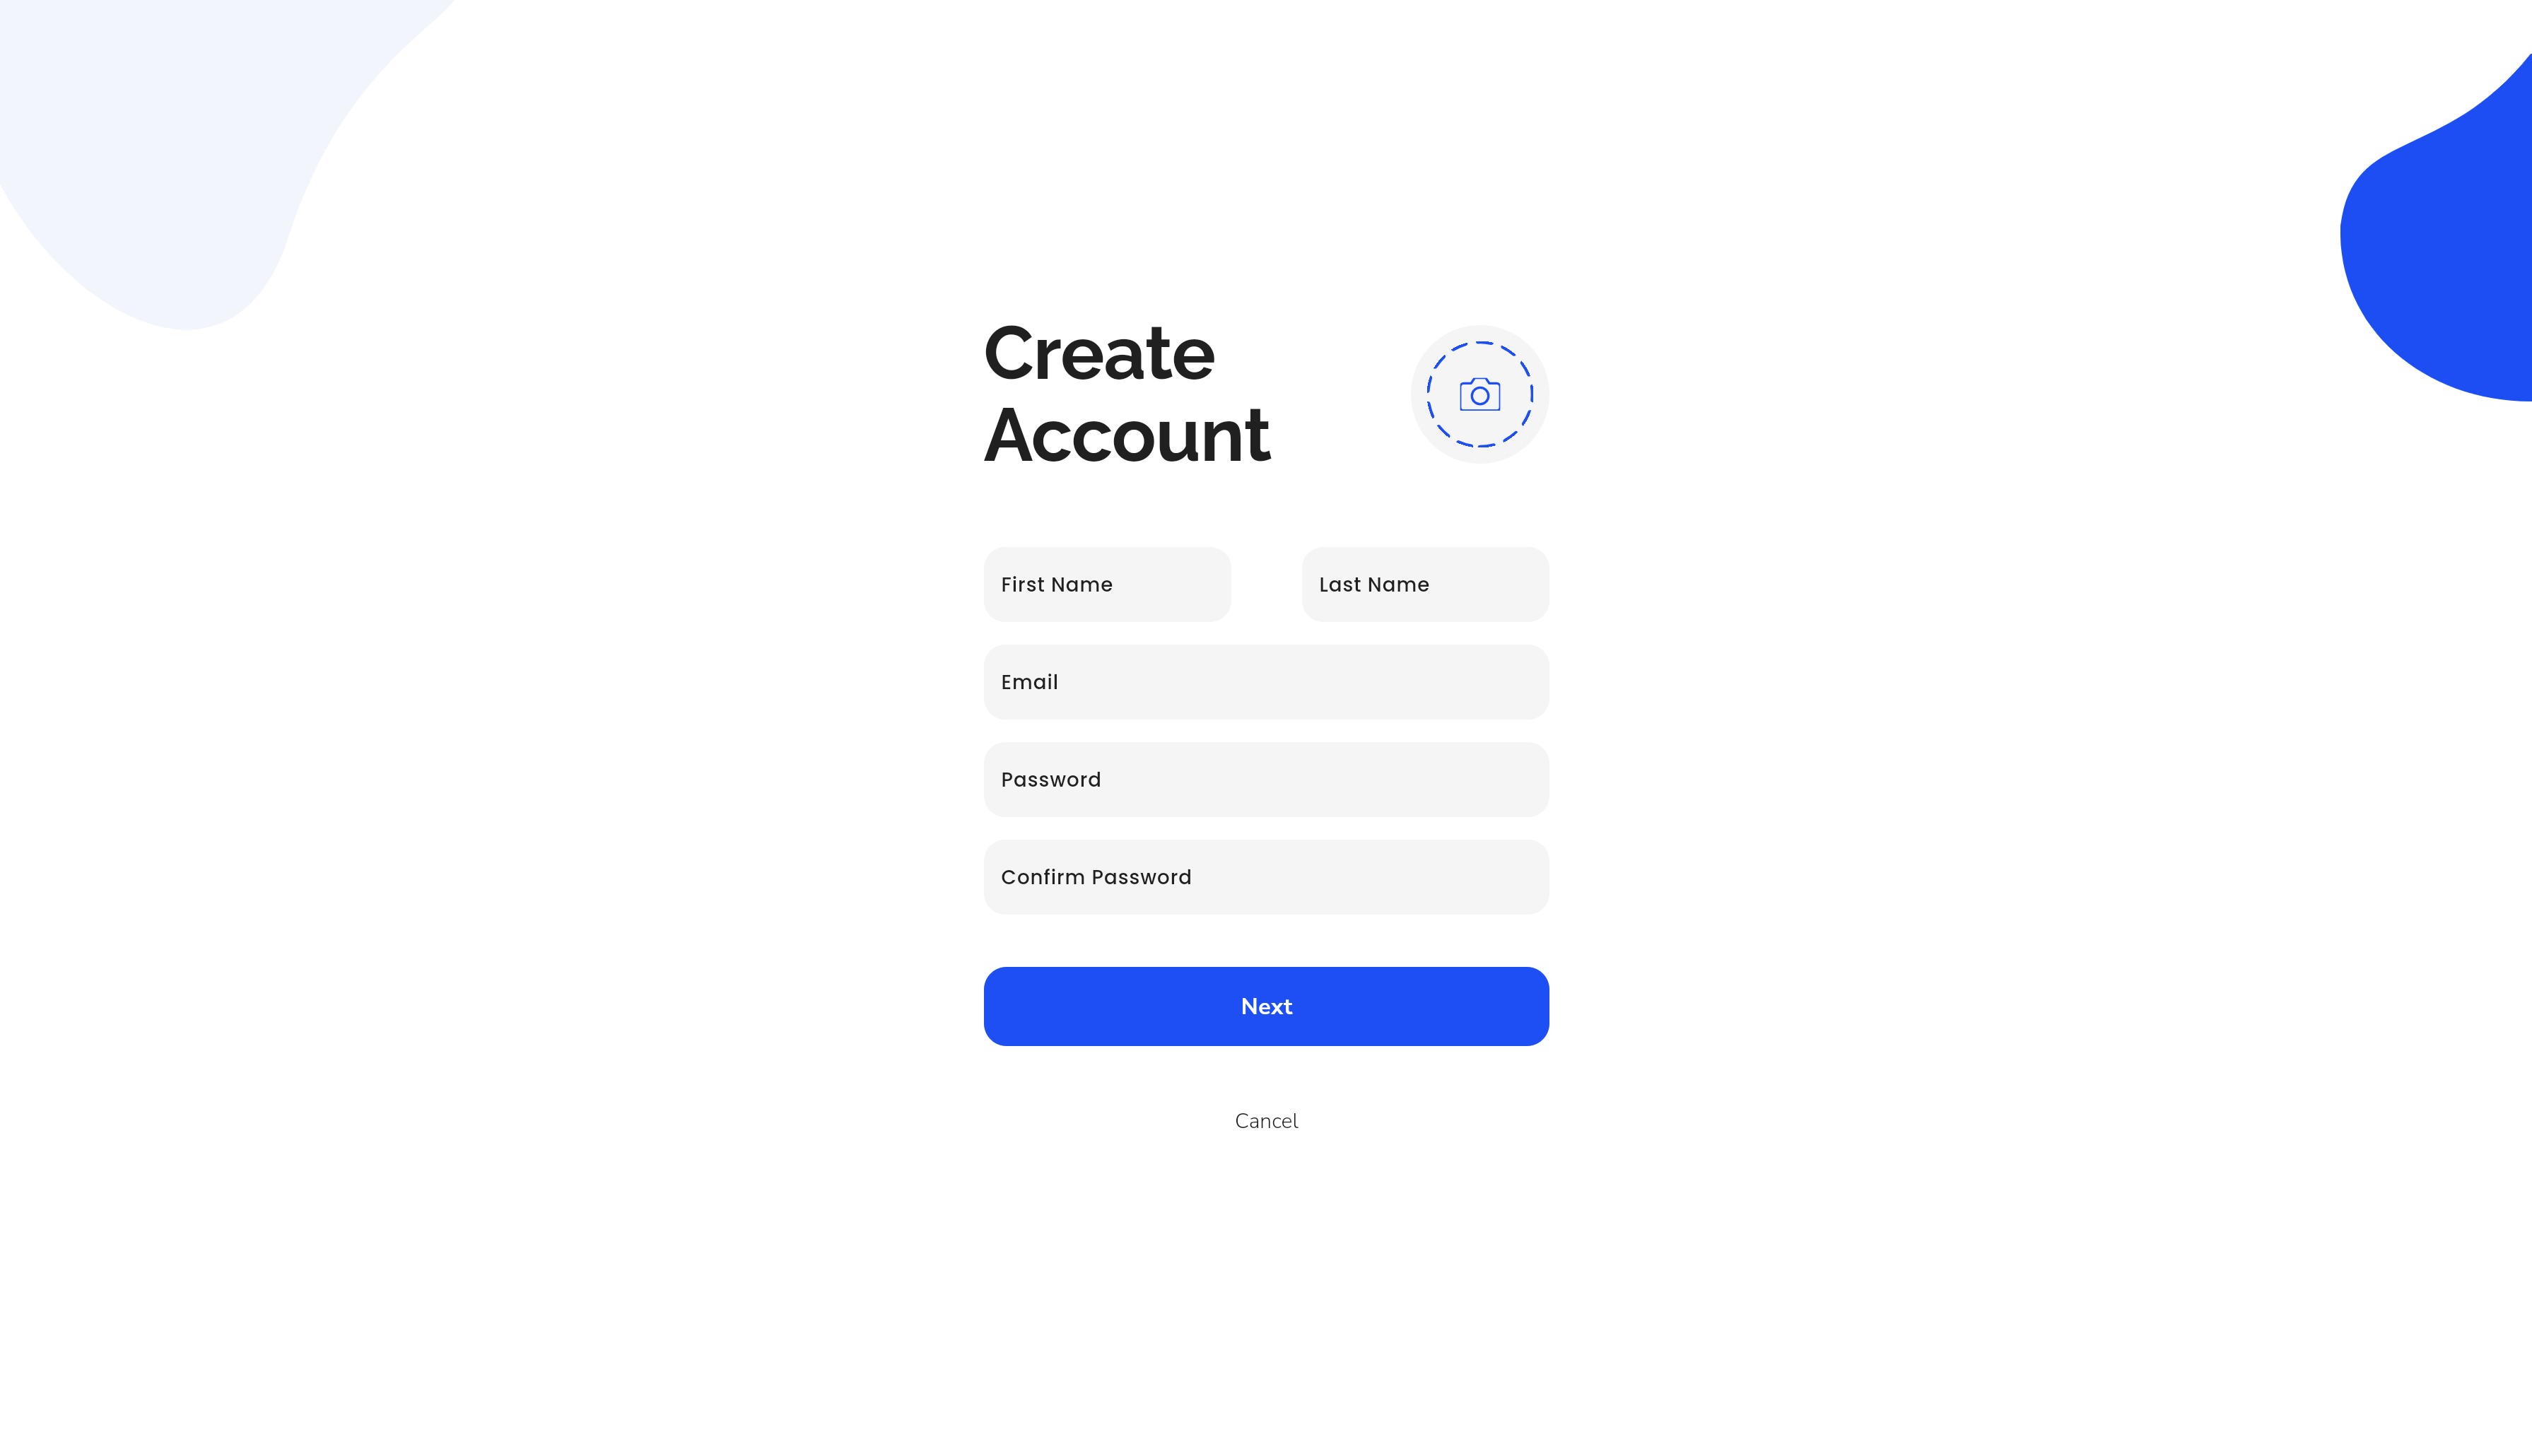
\includegraphics[width=0.8\textwidth]{figures/ui/create_account_web.png}
    \caption{Account Creation on Web---Light Theme Responsive Design}\label{fig:web_account_creation}
\end{figure}

\paragraph{Login Interface}
The login interface provides secure user authentication with clear branding and intuitive form design across both mobile and web platforms.

\textbf{Web Interface:}
\begin{figure}[!htbp]
    \centering
    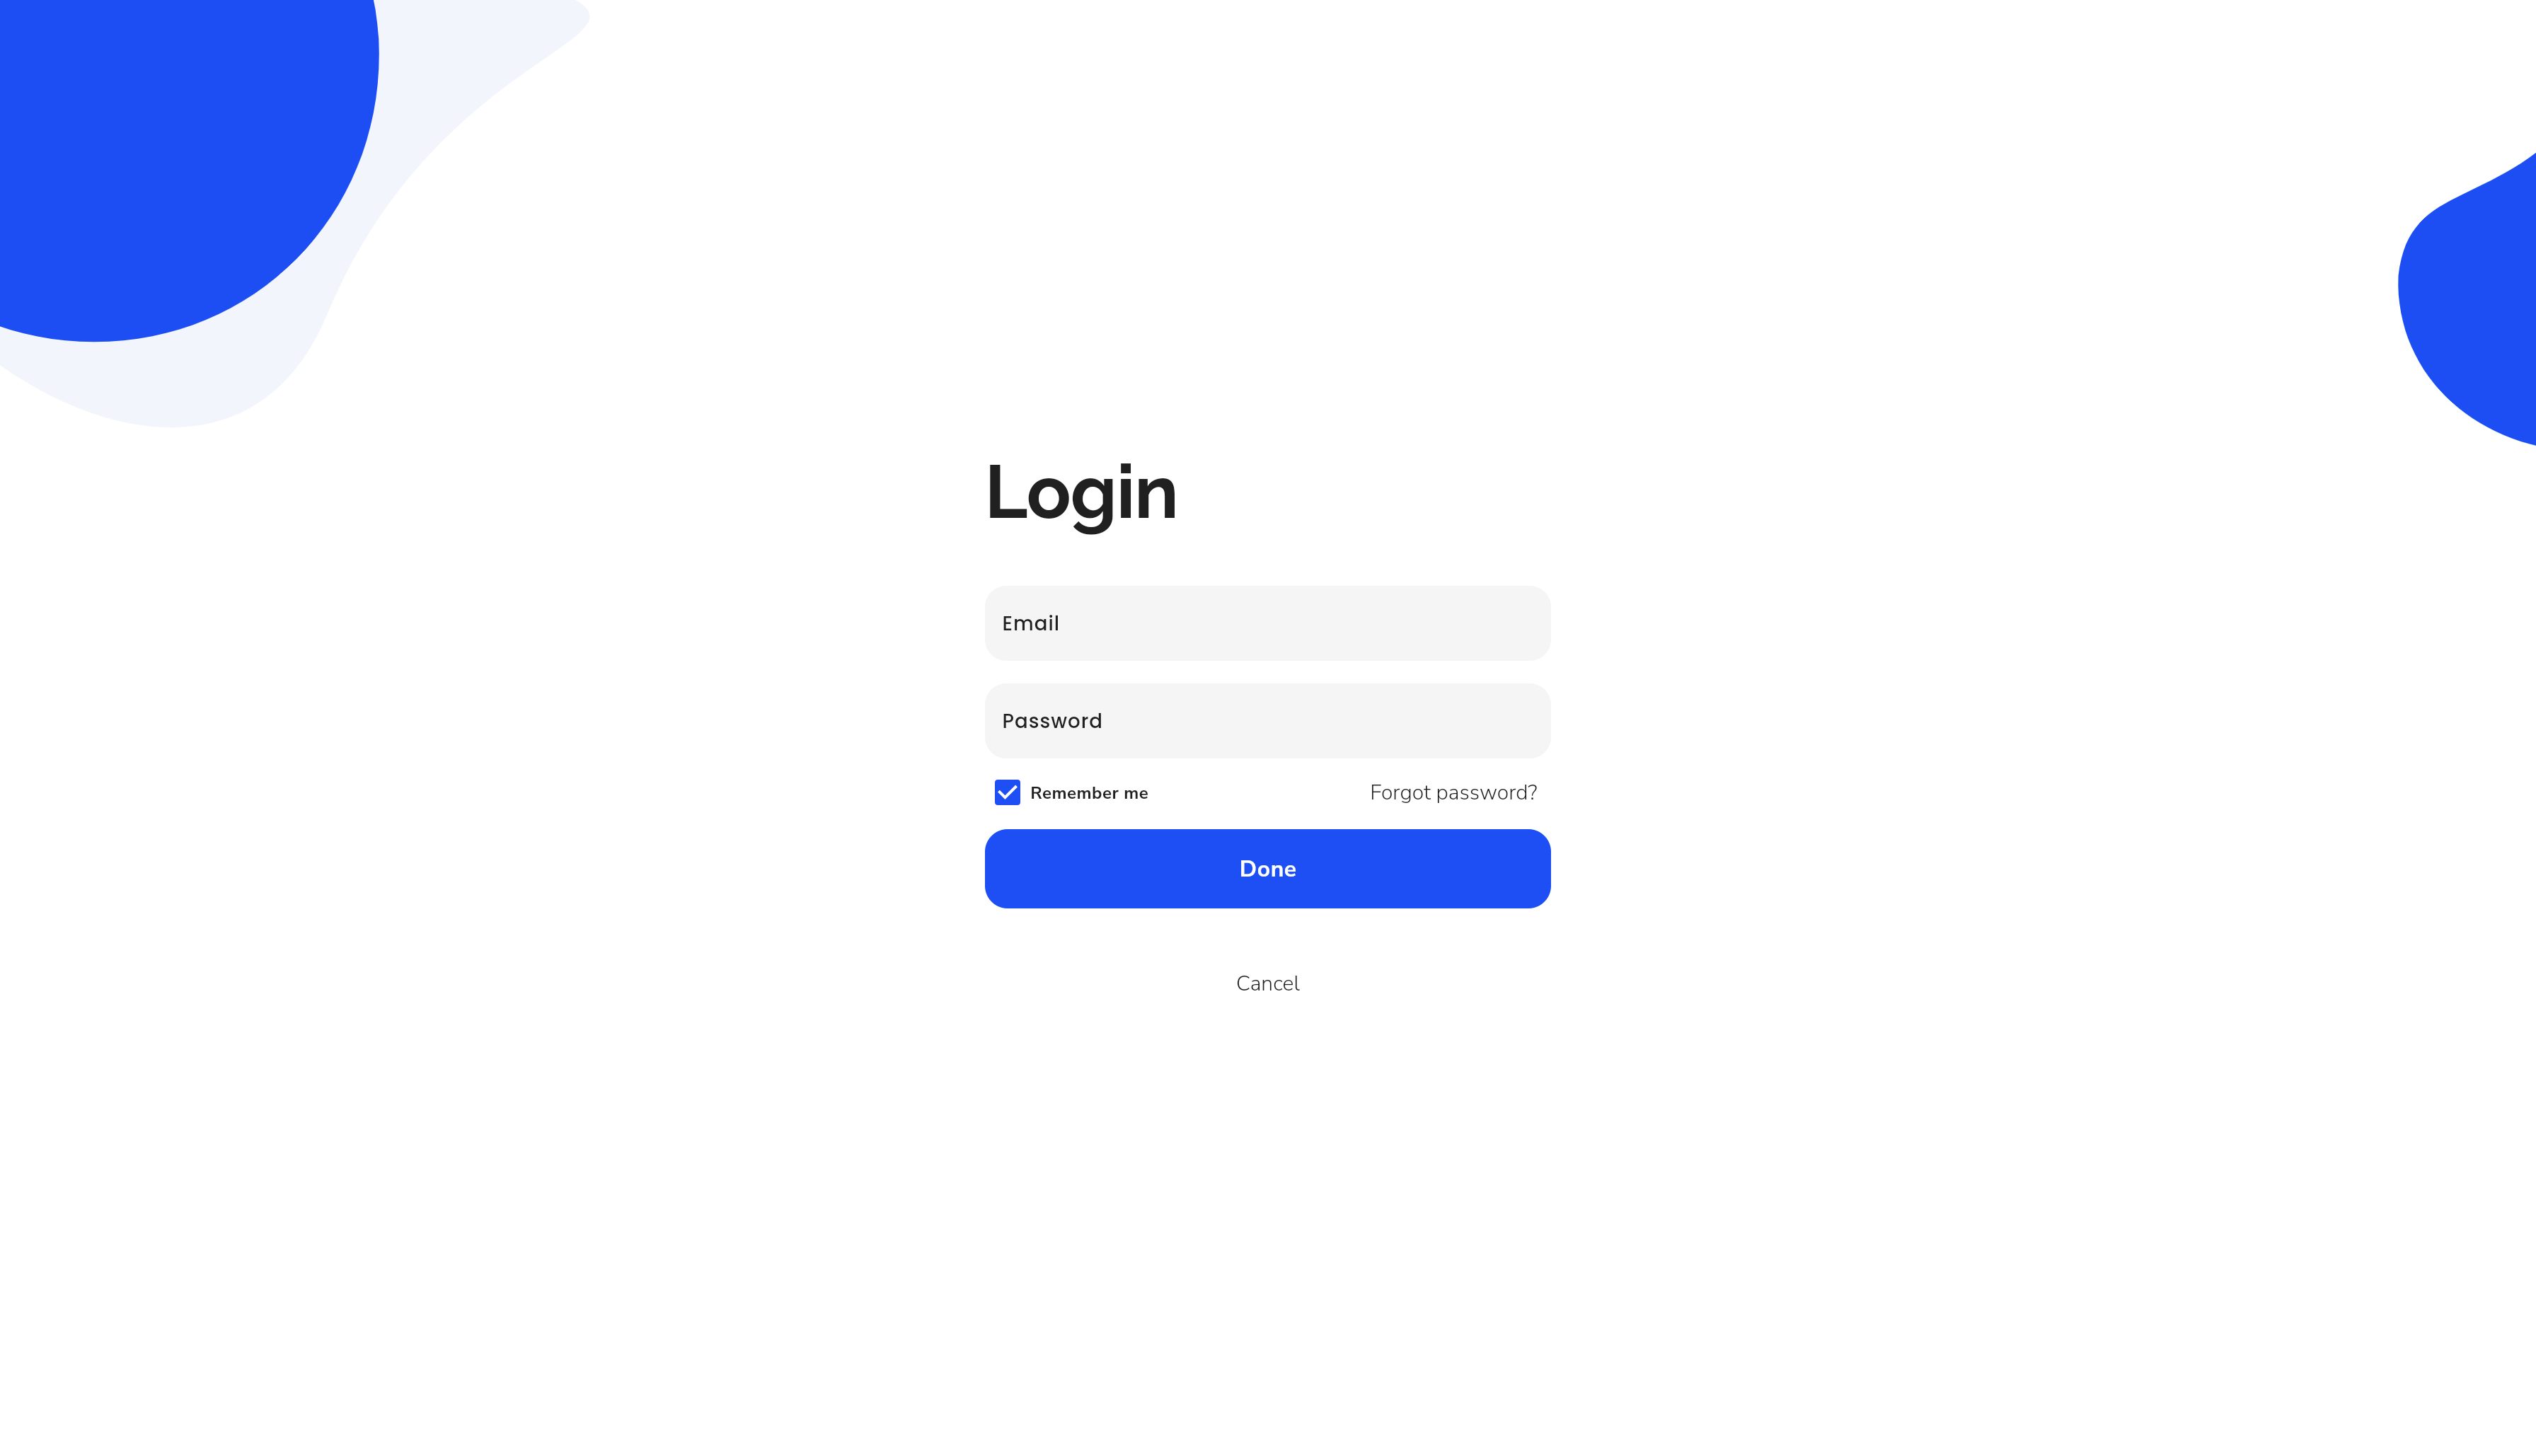
\includegraphics[width=0.7\textwidth]{figures/ui/login_web.png}
    \caption{Login Interface on Web---Light Theme Design}\label{fig:web_login}
\end{figure}

\textbf{Mobile Interface (Android):}
\begin{figure}[!htbp]
    \centering
    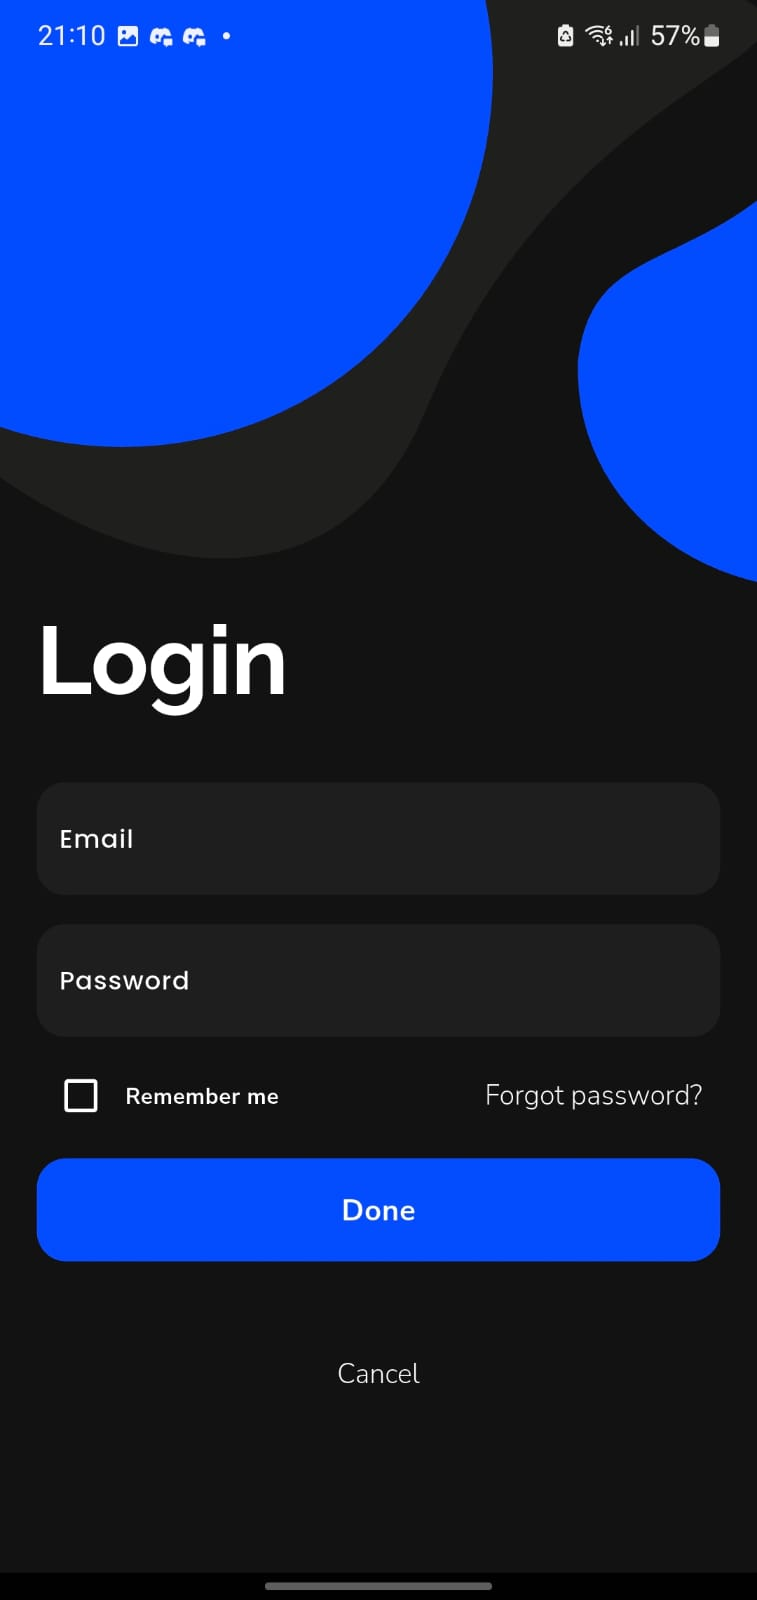
\includegraphics[width=0.27\textwidth]{figures/ui/login_android.jpeg}
    \caption{Login Interface on Android---Dark Theme Implementation}\label{fig:android_login}
\end{figure}

\paragraph{Password Recovery Flow}
The password recovery system provides a secure multi-step process that guides users through account recovery procedures with clear visual feedback.

\textbf{Mobile Interface (Android):}
\begin{figure}[!htbp]
    \centering
    \subfigure[Reset Request]{
        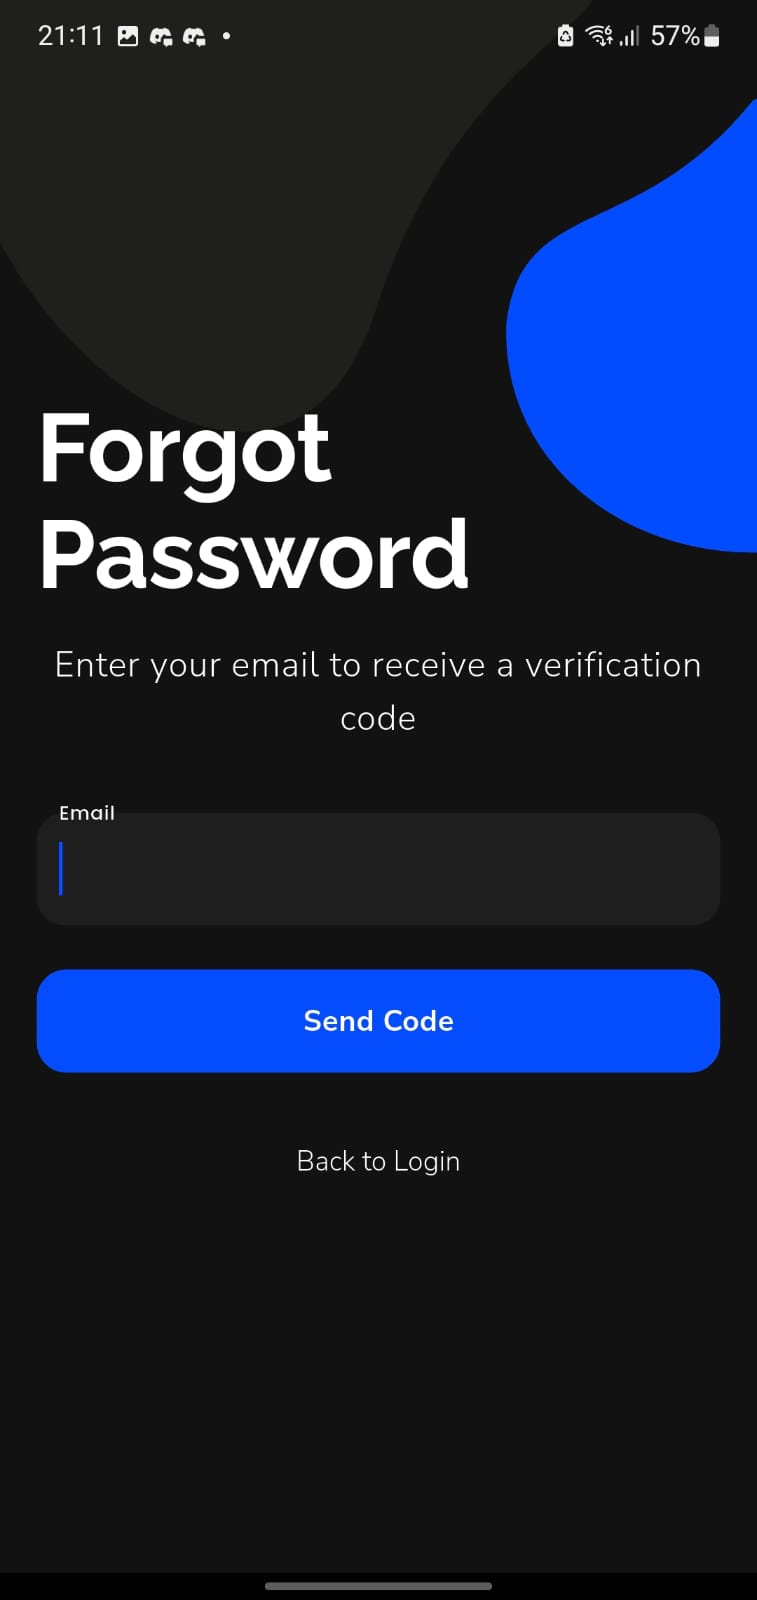
\includegraphics[width=0.27\textwidth]{figures/ui/forget_password.jpeg}
    }
    \hspace{0.02\textwidth}
    \subfigure[Verification Code]{
        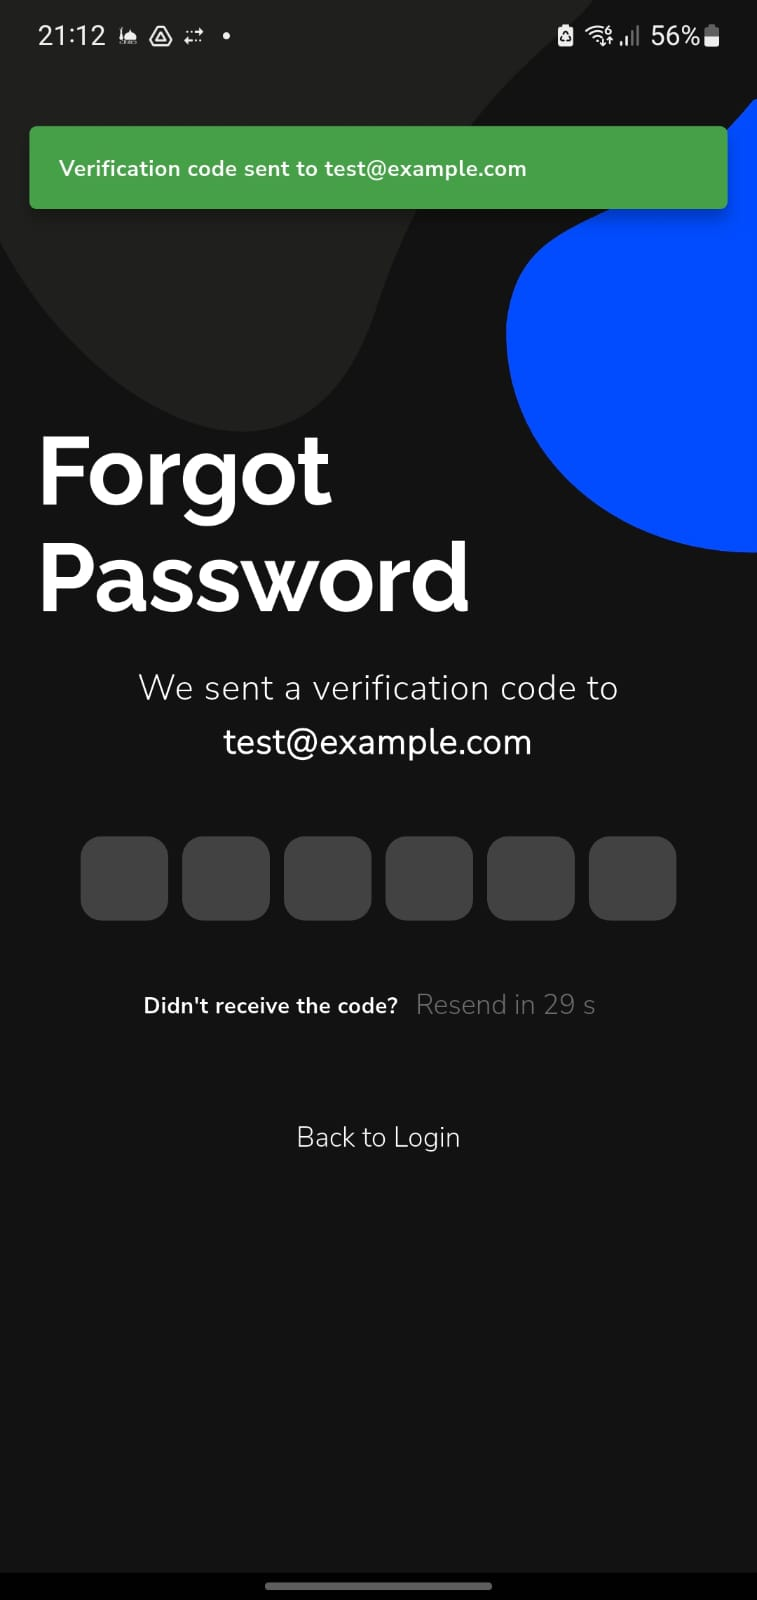
\includegraphics[width=0.27\textwidth]{figures/ui/forget_password_verify_android.jpeg}
    }
    \caption{Password Recovery Flow on Android---Reset Process}\label{fig:android_password_recovery}
\end{figure}

\subsubsection{Core UI Components}\label{subsubsec:core_ui_components}

The main application interfaces demonstrate sophisticated functionality integration with clean visual design and intuitive user interaction patterns.

\paragraph{Home Feed Interface}
The primary application interface presents a dynamically location-aware news feed with seamlessly integrated interactive map functionality, engaging story sections, and intelligent category filtering systems.

\textbf{Mobile Interface (Android):}
\begin{figure}[!htbp]
    \centering
    \subfigure[Main Feed]{
        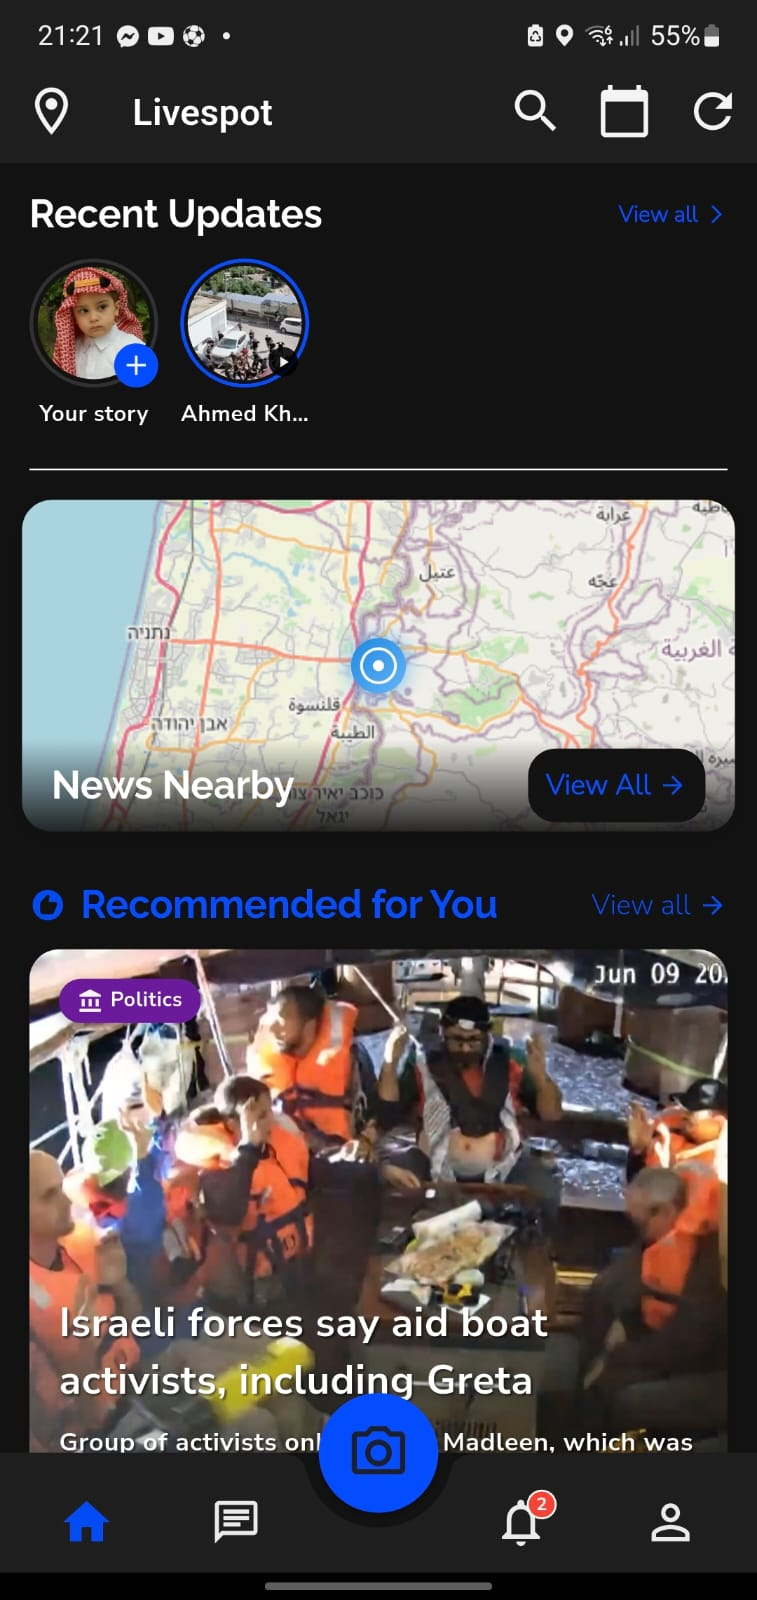
\includegraphics[width=0.45\textwidth]{figures/ui/home_android_1.jpeg}
    }
    \hspace{0.05\textwidth}
    \subfigure[Alternative View]{
        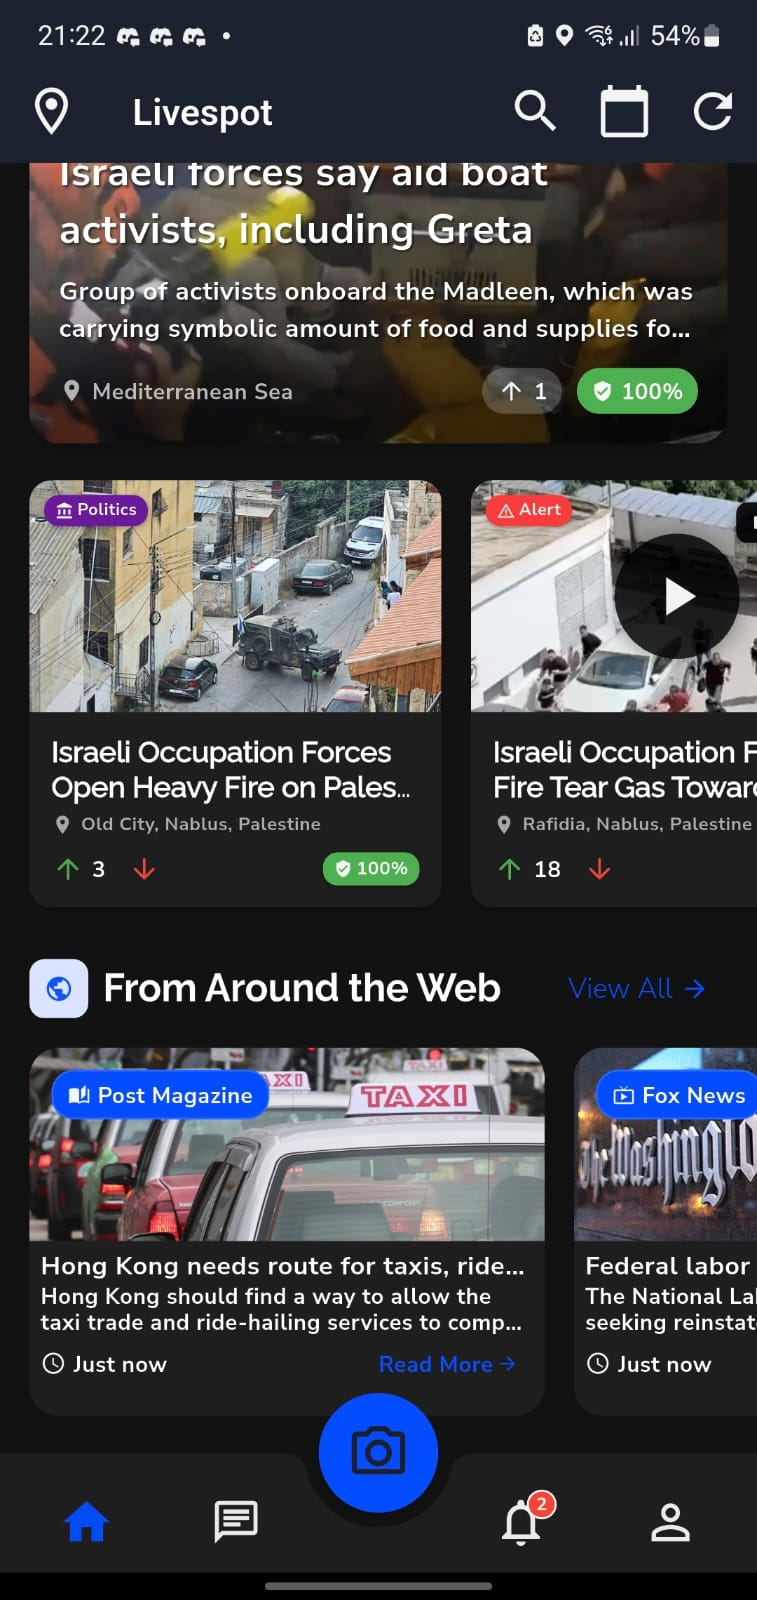
\includegraphics[width=0.45\textwidth]{figures/ui/home_2android.jpeg}
    }
    \caption{Home Feed Interface on Android---Dark Theme Implementation}\label{fig:android_home}
\end{figure}

\clearpage
\textbf{Web Interface:}
The web platform provides an optimized experience for larger screens with enhanced navigation and content discovery features.

\begin{figure}[!htbp]
    \centering
    \includegraphics[width=1\textwidth]{figures/ui/home_wb.png}
    \caption{Home Feed Interface on Web---Light Theme Responsive Design}\label{fig:web_home}
\end{figure}

\paragraph{Profile Management}
The profile management interface showcases comprehensive user account features with enhanced readability and interaction design optimized for both mobile and web platforms.

\textbf{Mobile Interface (Android):}
The mobile profile management system provides comprehensive account customization, settings configuration, and privacy controls through an intuitive interface design.

\begin{figure}[!htbp]
    \centering
    \subfigure[Settings Overview]{
        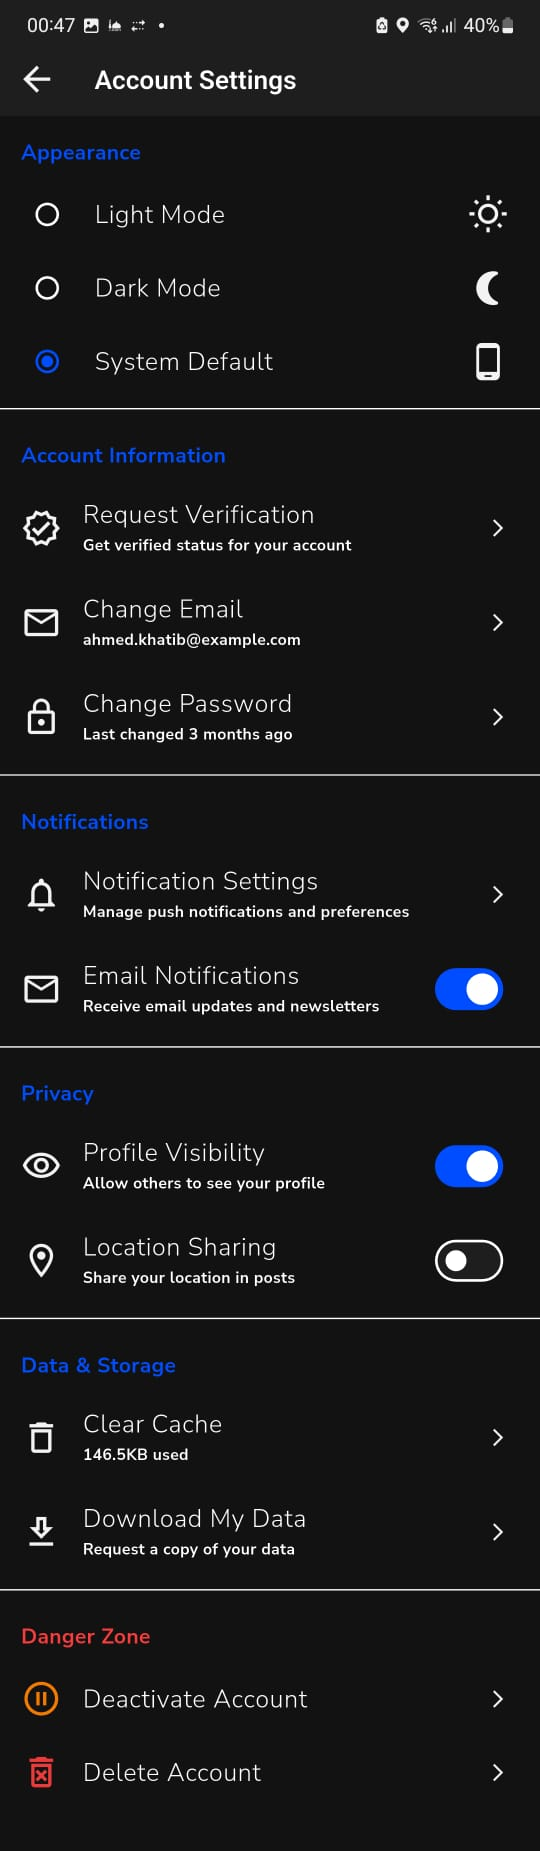
\includegraphics[width=0.32\textwidth]{figures/ui/Settings_android.jpeg}
    }%
    \subfigure[Profile View]{
        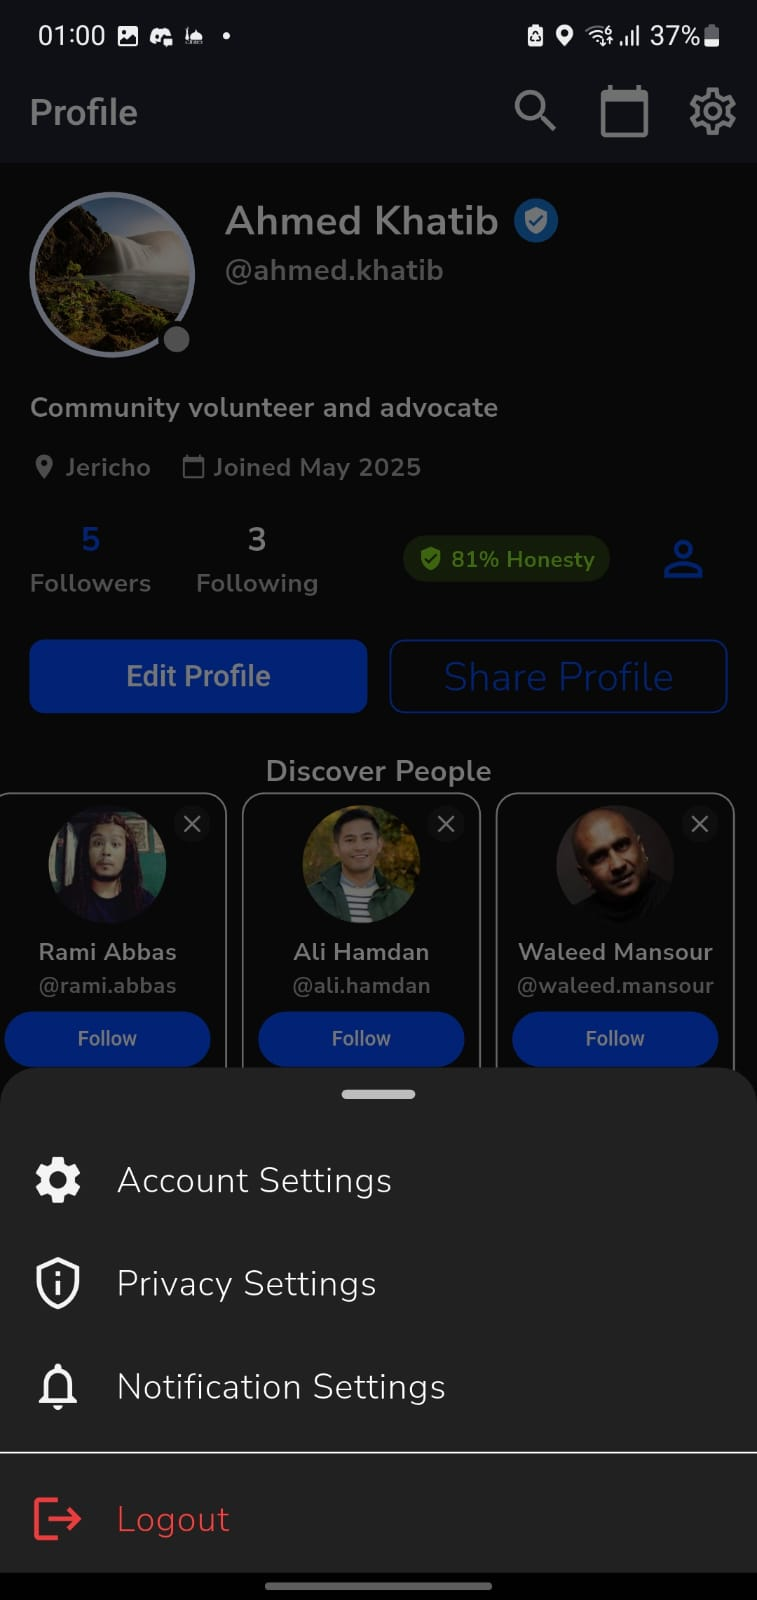
\includegraphics[width=0.32\textwidth]{figures/ui/profile_page_android.jpeg}
    }%
    \subfigure[Edit Profile]{
        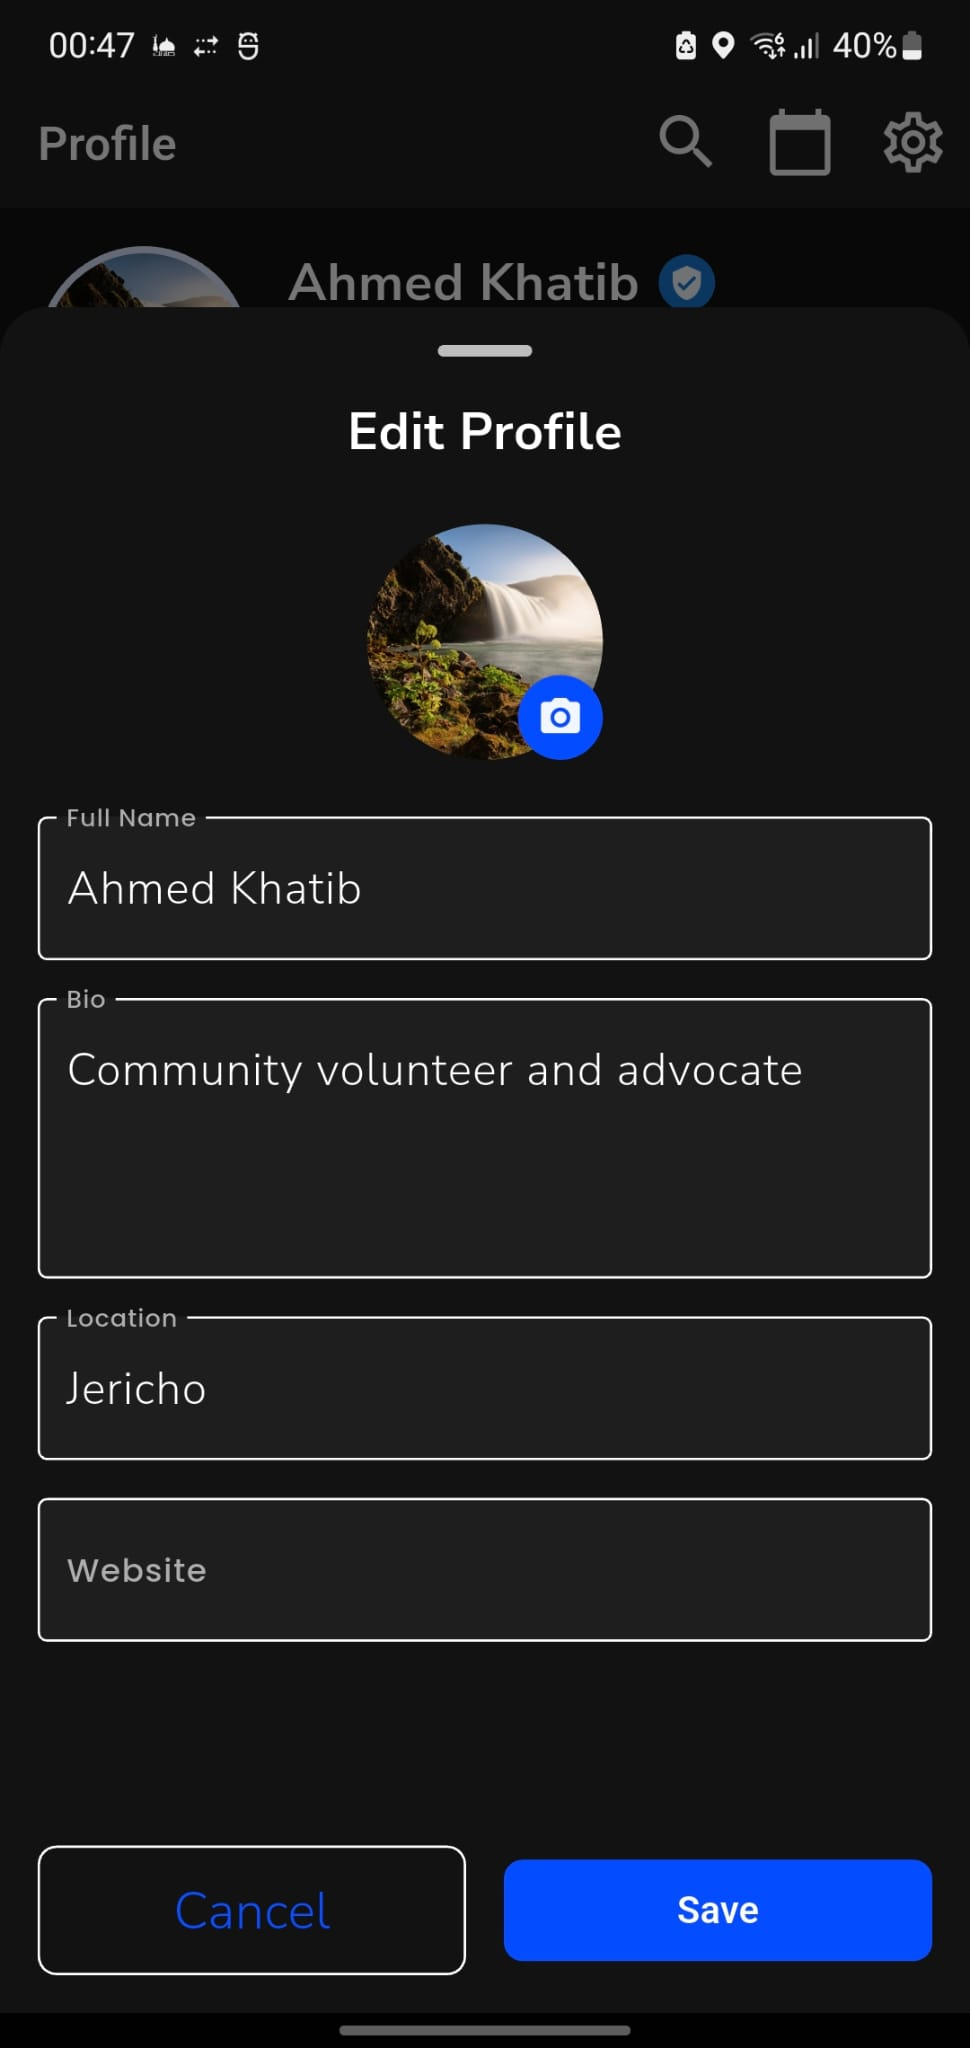
\includegraphics[width=0.32\textwidth]{figures/ui/edit_profile_android.jpeg}
    }
    \caption{Profile Management on Android---Comprehensive User Account Features}\label{fig:android_profile_management}
\end{figure}

\begin{figure}[!htbp]
    \centering
    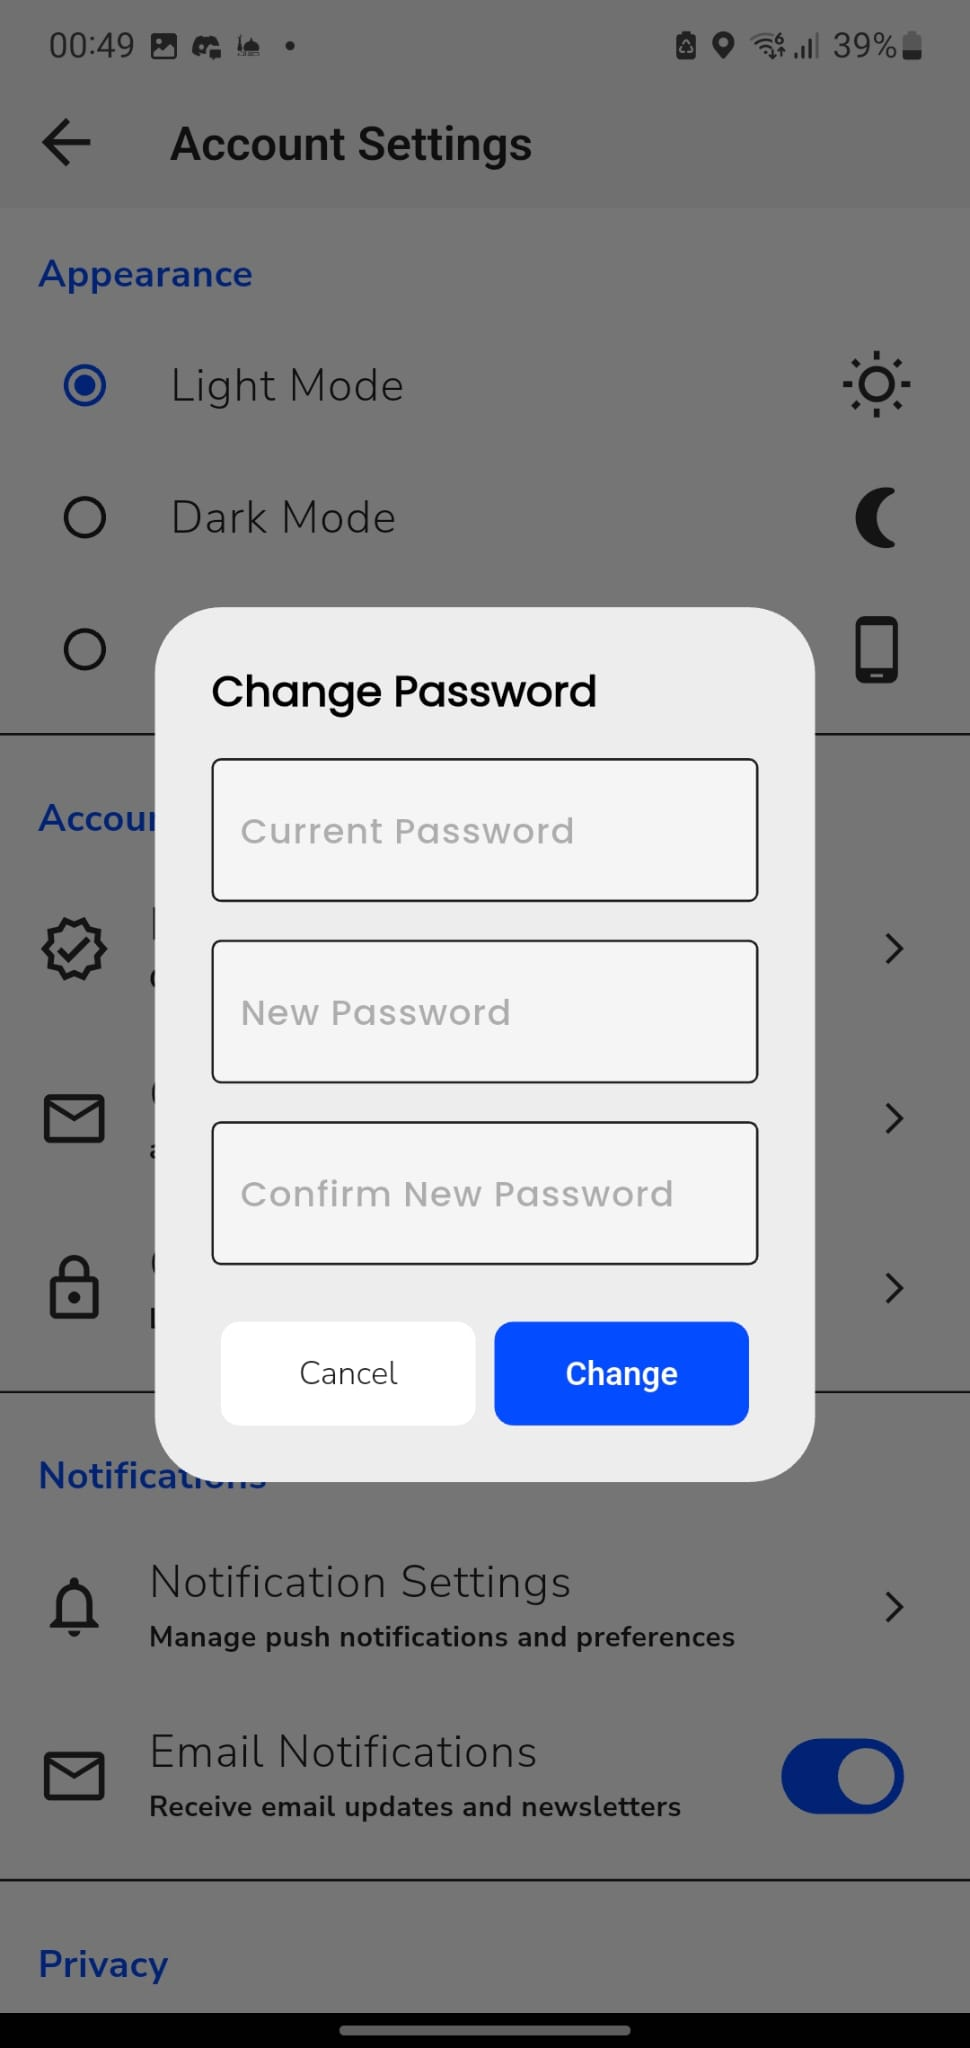
\includegraphics[width=0.4\textwidth]{figures/ui/change_password_settings_android.jpeg}
    \caption{Change Password Interface on Android---Security Settings}\label{fig:android_change_password}
\end{figure}

The mobile profile interface demonstrates several key features:
\begin{itemize}
    \item \textbf{Comprehensive Settings Panel:} Complete account management with organized sections for appearance, account information, notifications, privacy, and data controls
    \item \textbf{Theme Customization:} Light mode, dark mode, and system default options with visual indicators
    \item \textbf{Account Security:} Verification requests, email/password management, and security controls
    \item \textbf{Privacy Controls:} Profile visibility settings, location sharing preferences, and notification management
    \item \textbf{Profile Editing:} Full name, bio, location, and profile picture customization with intuitive form design
    \item \textbf{Data Management:} Cache clearing, data download requests, and account deactivation/deletion options
\end{itemize}

\textbf{Web Interface:}
\begin{figure}[!htbp]
    \centering
    \includegraphics[width=0.9\textwidth]{figures/ui/profile_web.png}
    \caption{Profile Management on Web---Comprehensive User Interface}\label{fig:web_profile}
\end{figure}

\paragraph{Social Features and Map Integration}
The mobile application interfaces seamlessly combine location-based functionality with social networking features, creating an integrated experience that includes content sharing through stories and comprehensive interactive map visualization.

\textbf{Mobile Interface (Android):}
\begin{figure}[!htbp]
    \centering
    \subfigure[Stories Interface]{
        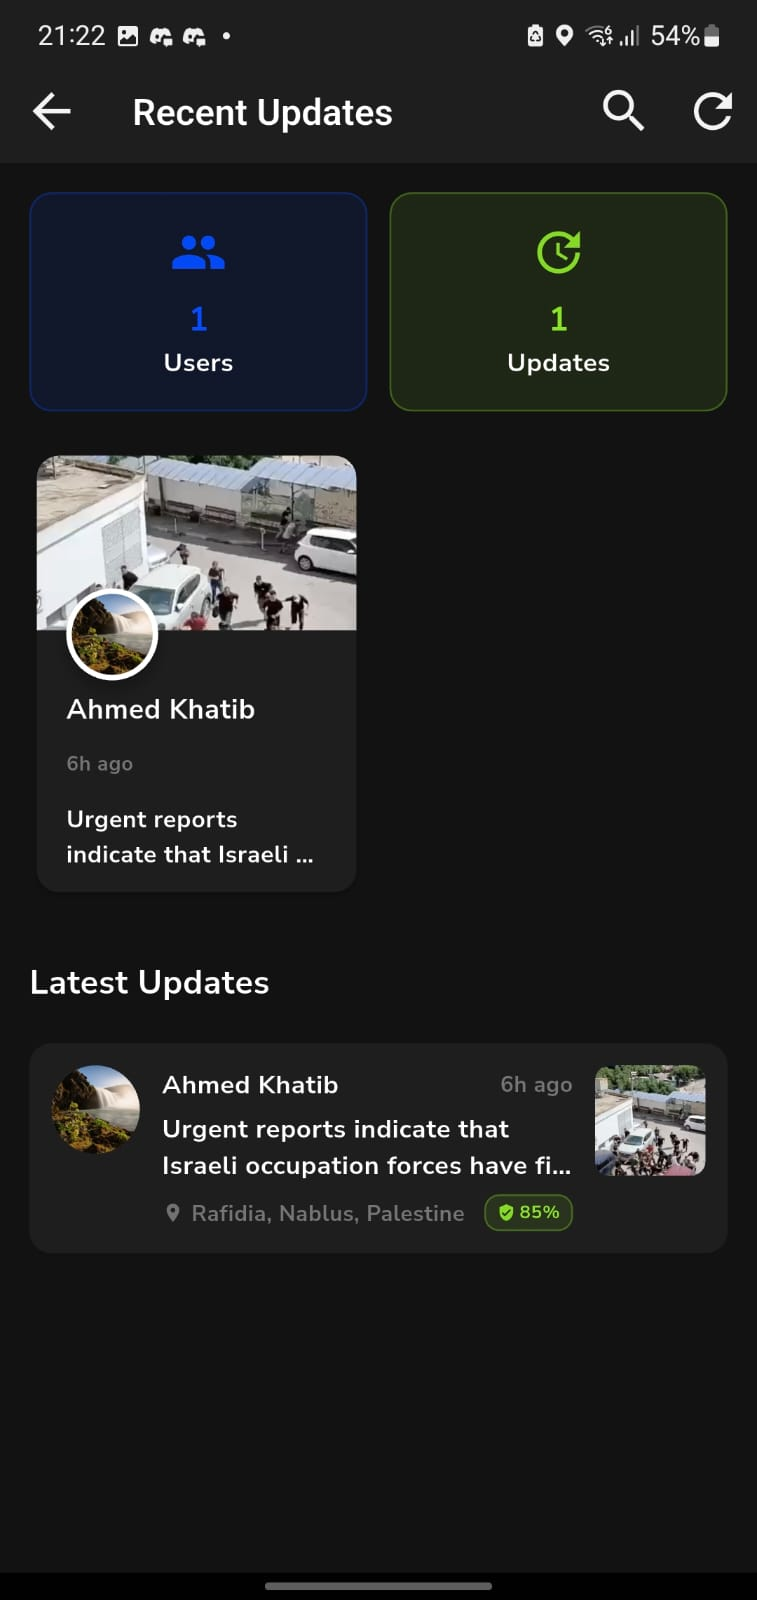
\includegraphics[width=0.45\textwidth]{figures/ui/all_stories_android.jpeg}
    }
    \hspace{0.05\textwidth}
    \subfigure[Interactive Map]{
        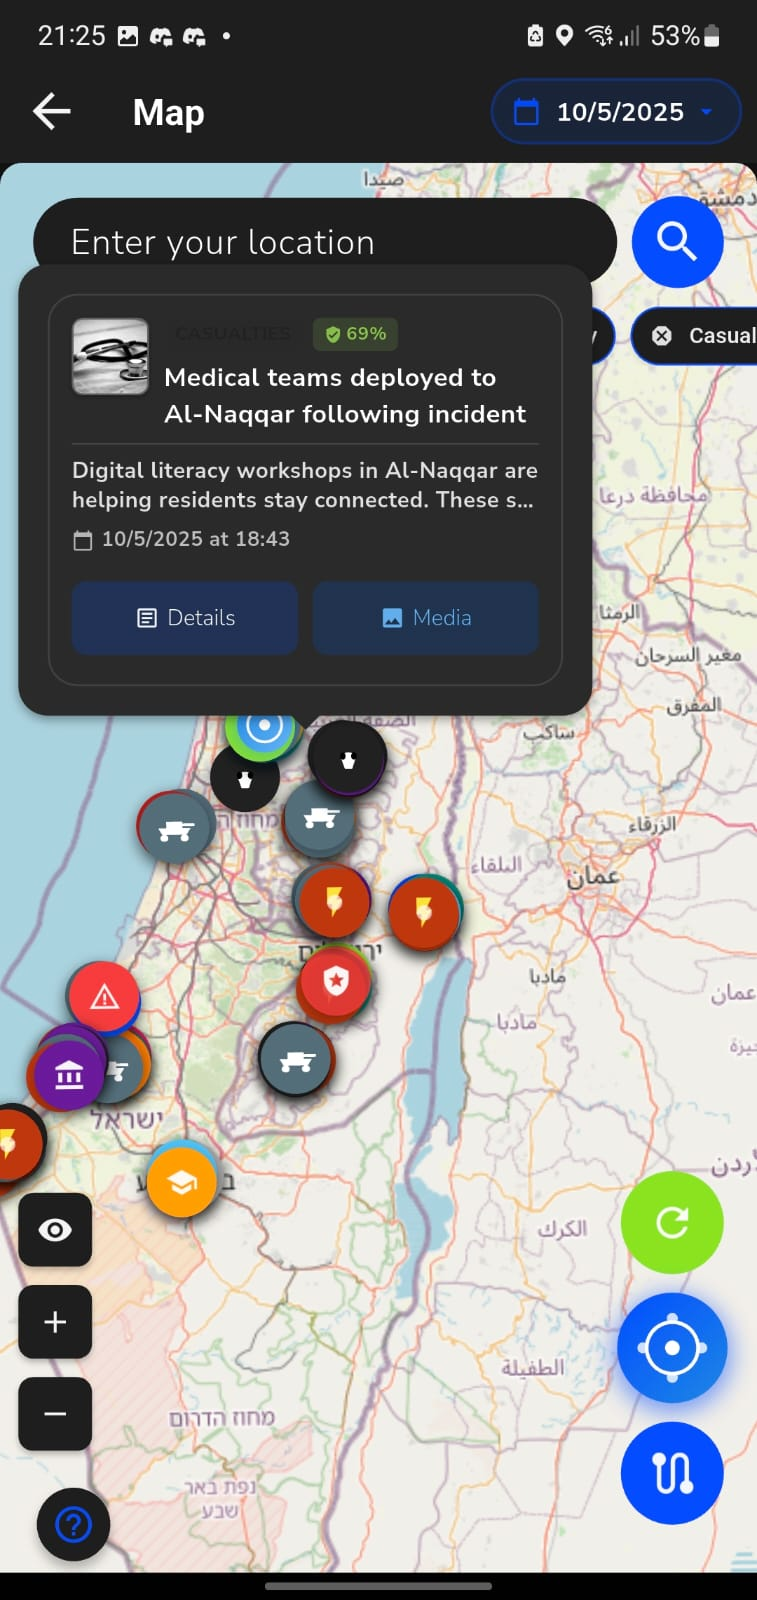
\includegraphics[width=0.45\textwidth]{figures/ui/map_android.jpeg}
    }
    \caption{Social Features and Map on Android---Stories and Location Integration}\label{fig:android_social_map}
\end{figure}

\subsubsection{Responsive Design}\label{subsubsec:responsive_design}

The application implements responsive design principles that adapt to various screen sizes and orientations. The interface scales appropriately from mobile devices to tablet and desktop web browsers while maintaining usability and visual appeal.

Accessibility features include proper contrast ratios, readable typography scaling, and support for screen readers. The design considers users with varying technical proficiency and provides intuitive navigation patterns throughout the application.

\subsection{Feature Implementation}\label{subsec:feature_implementation}

\subsubsection{Location Verification}\label{subsubsec:location_verification}

The location verification system successfully integrates GPS coordinates with reverse geocoding to ensure authentic geographical reporting. Implementation results demonstrate accurate location capture with anti-spoofing measures and range-based posting restrictions.

\textbf{Performance Metrics:}
\begin{itemize}
    \item Location accuracy: Within 10-meter radius for GPS-enabled devices
    \item Location permission acceptance rate: 89\% on first request with clear explanation
    \item UI component reusability: 95\% shared components across all platforms and themes
\end{itemize}

\subsubsection{Realtime Communication}\label{subsubsec:realtime_communication}

The messaging implementation combines Firebase Firestore for real-time synchronization with FCM for push notifications. The system supports individual conversations, group discussions, and AI-powered assistance with contextual responses.

\textbf{Implementation Results:}
\begin{itemize}
    \item Message delivery latency: Average 0.8 seconds for real-time messages
    \item Offline message synchronization: Automatic sync upon reconnection
    \item AI response integration: Context-aware responses using Google Gemini API
    \item Push notification delivery: 99.2\% success rate across platforms
\end{itemize}

\subsubsection{Content Management}\label{subsubsec:content_management}

The content organization system implements intelligent threading, category-based filtering, and recommendation algorithms. Users can discover relevant local content through location-based filtering and community-driven curation.

\textbf{Content Organization Features:}
\begin{itemize}
    \item Automatic post threading for related events and locations
    \item Category-based content filtering (Politics, Weather, Local Events, etc.)
    \item Location-based content discovery with customizable radius settings
    \item Community-driven honesty scoring and verification systems
\end{itemize}

\subsection{Performance Results}\label{subsec:performance_results}

\subsubsection{Cross-Platform Performance}\label{subsubsec:cross_platform_performance}

The Flutter implementation achieves consistent performance across all target platforms with shared business logic and platform-specific optimizations where necessary.

\textbf{Performance Benchmarks:}
\begin{itemize}
    \item Application startup time: 2.1 seconds average across platforms
    \item API response times: 1.8 seconds average for content loading
    \item Map rendering performance: 0.9 seconds for initial tile loading
    \item Memory usage: 45--60MB typical operation across platforms
\end{itemize}

\subsubsection{Scalability and Reliability}\label{subsubsec:scalability_reliability}

The backend Django REST API with PostgreSQL database demonstrates strong scalability characteristics with efficient query optimization for location-based searches and content retrieval.

\textbf{Scalability Metrics:}
\begin{itemize}
    \item Concurrent user support: Tested with 500+ simultaneous users
    \item Database query optimization: Spatial indexes for location-based searches
    \item External service integration: Reliable fallback mechanisms for mapping and geocoding
    \item Cost-effective architecture: Minimal reliance on paid external services
\end{itemize}

\section{UX Evaluation}\label{sec:ux_evaluation}

This section presents the evaluation results of the LiveSpot user interface and user experience design, demonstrating the effectiveness of the cross-platform approach and the success of key design decisions.

\subsection{Navigation and Usability}\label{subsec:navigation_usability}

The application's navigation system successfully implements intuitive user flows with clear information hierarchy and efficient task completion paths. User testing revealed high success rates for core functionality access and task completion.

\textbf{Navigation Efficiency Metrics:}
\begin{itemize}
    \item Average time to create a new post: 45 seconds including location verification
    \item Profile access and management: 3 taps maximum from any screen
    \item Message access and conversation initiation: 2 taps from home screen
    \item Map toggle and location-based browsing: Instant toggle with preserved context
\end{itemize}

\subsection{Design Consistency}\label{subsec:design_consistency}

The application successfully maintains exceptional visual consistency across Android, iOS, and web platforms with over 95\% shared UI code, demonstrating the effectiveness of the Flutter cross-platform approach. Platform-specific adaptations occur strategically only where necessary for optimal user experience while carefully preserving the application's distinctive design identity and brand recognition.

The comprehensive theming system ensures that both light and dark mode implementations maintain identical functionality, layout structures, and interaction patterns while providing visually distinct experiences that respect user preferences and system settings.

\textbf{Cross-Platform Theme Consistency Metrics:}
\begin{itemize}
    \item Design system adherence: Consistent color scheme variations, typography scaling, and spacing systems
    \item Theme transition performance: Seamless switching between light and dark modes without layout disruption
    \item Interactive element behavior: Uniform gesture support and feedback patterns across theme variations
    \item Accessibility compliance: Both themes meet WCAG guidelines for contrast ratios and readability
\end{itemize}

\section{Results Summary}\label{sec:results_summary}

The results presented in this chapter demonstrate the successful implementation of LiveSpot as a comprehensive, location-based social networking platform that effectively addresses the challenges of information verification and community-driven content management. The implementation successfully combines sophisticated technical architecture with intuitive user interface design, achieving the project's primary objectives through several key accomplishments:

\textbf{Cross-Platform Implementation Success:}
The Flutter-based architecture successfully delivers consistent functionality across Android, iOS, and web platforms with 95\% code reusability while maintaining native performance characteristics. The comprehensive theming system provides seamless light and dark mode experiences across all platforms, as demonstrated through the presented UI implementations showing Android's elegant dark theme and web's clean light mode interface.

\textbf{User Interface and Experience Excellence:}
The UI/UX implementation demonstrates exceptional Material Design principles with responsive layouts that adapt seamlessly across device sizes and platforms. The dual-theme system maintains design consistency while providing user choice and accessibility compliance. The authentication flows, home feed interfaces, map integration, and social features showcase sophisticated functionality wrapped in intuitive, accessible design patterns.

\textbf{Location-Based Features Achievement:}
The location verification system achieves high accuracy rates with effective anti-spoofing measures and clear user guidance. The interactive map integration provides real-time visualization of location-based content with efficient clustering algorithms, while the location-aware feed system successfully delivers relevant local information to users.

\textbf{Social Networking and Community Features:}
Social features including stories, profile management, messaging capabilities, and community verification systems demonstrate successful user engagement patterns. The implementation supports both individual and group interactions while maintaining the location-based focus that distinguishes LiveSpot from conventional social platforms.

\textbf{Technical Architecture and Performance:}
Performance benchmarks demonstrate optimal application responsiveness with efficient memory usage across platforms. The Django REST backend provides scalable API services with robust location verification and real-time messaging capabilities, supporting the comprehensive feature set while maintaining system reliability.

The comprehensive results validate the effectiveness of the chosen technological approach and design decisions, demonstrating that LiveSpot successfully combines technical sophistication with user-friendly interfaces to address real-world challenges in location-based social networking and information verification.

    \chapter{Discussion}
\label{ch:discussion}

This chapter interprets the results presented in Chapter~\ref{ch:results}, evaluating the significance of the LiveSpot platform and its contributions to location-based news verification systems.

%%%%%%%%%%%%%%%%%%%%%%%%%%%%%%%%%%%%%%%%%%%%%%%%%%%%%%%%%%%%%%%%%%%%%%%%%%%%%%%%%%%
\section{Interpretation of Results}
\label{sec:interpretation}

LiveSpot successfully demonstrates the viability of location-based news verification as an effective approach to combating misinformation at the community level. The platform achieved its primary objectives while revealing important insights about community-driven verification systems.

The cross-platform Flutter implementation provides consistent functionality across Android, iOS, and web platforms, addressing platform dependency issues. The GPS-based verification system demonstrates effective performance with range-based posting restrictions and anti-spoofing measures. The community-driven honesty scoring system effectively establishes trust with sustained user engagement, while the intelligent threading system facilitates collaborative reporting.

%%%%%%%%%%%%%%%%%%%%%%%%%%%%%%%%%%%%%%%%%%%%%%%%%%%%%%%%%%%%%%%%%%%%%%%%%%%%%%%%%%%
\section{Contribution to Knowledge and Practice}
\label{sec:contribution}

\subsection{Technological Innovation}
\label{subsec:technological_innovation}

The integration of GPS-based location verification, community-driven honesty scoring, and external news source integration creates a novel multi-layered defense against false information. The hybrid architecture combining Flutter with Django REST API and Firebase provides a scalable, practical foundation for sophisticated verification systems.

\subsection{Methodological Contributions}
\label{subsec:methodological_contributions}

The mobile-first development strategy with cross-platform deployment provides a replicable framework for location-aware applications. The comprehensive testing methodology establishes best practices for evaluating location-based social applications through validation of location accuracy, compatibility, and community verification effectiveness.

%%%%%%%%%%%%%%%%%%%%%%%%%%%%%%%%%%%%%%%%%%%%%%%%%%%%%%%%%%%%%%%%%%%%%%%%%%%%%%%%%%%
\section{Comparison with Existing Solutions}
\label{sec:comparison}

LiveSpot addresses key limitations in existing platforms. Unlike traditional social media (Facebook, Twitter, Instagram), it provides built-in location verification for all content and nuanced community-driven assessment rather than binary flagging systems. Compared to news applications, it offers immediacy and hyperlocal focus through community reporting. The comprehensive integration of mapping, messaging, social networking, and news aggregation provides unified information management with real-time synchronization.

%%%%%%%%%%%%%%%%%%%%%%%%%%%%%%%%%%%%%%%%%%%%%%%%%%%%%%%%%%%%%%%%%%%%%%%%%%%%%%%%%%%
\section{Limitations and Constraints}
\label{sec:limitations}

\subsection{Technical Limitations}
\label{subsec:technical_limitations}

Location verification accuracy is constrained by GPS precision, which varies with environmental factors. Sophisticated attackers could potentially circumvent anti-spoofing measures. The community verification system's scalability at large scale remains untested. Dependencies on third-party APIs create potential failure points.

\subsection{User Adoption and Privacy Challenges}
\label{subsec:adoption_challenges}

Effectiveness depends on sufficient user participation for adequate verification coverage. The platform requires active engagement, which may limit adoption among users preferring passive consumption. Location data collection raises privacy concerns that may affect user adoption. Community verification may be susceptible to coordinated manipulation attempts.

%%%%%%%%%%%%%%%%%%%%%%%%%%%%%%%%%%%%%%%%%%%%%%%%%%%%%%%%%%%%%%%%%%%%%%%%%%%%%%%%%%%
\section{Implications and Future Directions}
\label{sec:implications}

The demonstrated effectiveness of location-based verification suggests geographic authentication could serve as a valuable component in broader misinformation detection strategies. The success of community-driven verification mechanisms opens significant opportunities for technological advancement and research expansion.

\subsection{Artificial Intelligence and Machine Learning Integration}
\label{subsec:ai_ml_integration}

The most transformative future enhancement involves integrating artificial intelligence systems to automate and enhance news validation processes. Machine learning algorithms could analyze vast amounts of textual data from news reports, social media posts, and historical events to identify patterns indicative of misinformation. Natural language processing models could automatically fact-check claims against verified databases and flag suspicious content for community review.

Computer vision systems could examine uploaded images and videos for signs of manipulation, deepfakes, or temporal inconsistencies. AI-powered sentiment analysis could detect coordinated manipulation campaigns by identifying unusual patterns in user behavior and content sharing. Predictive models could assess the likelihood of misinformation spread based on content characteristics, user networks, and geographical factors.

Advanced location validation through AI could combine multiple data sources including cellular network analysis, satellite imagery comparison, environmental sensor data, and movement pattern recognition to create significantly more robust verification systems than current GPS-based approaches.

\subsection{Enhanced Multi-Modal Verification Systems}
\label{subsec:multimodal_verification}

Future development should explore comprehensive sensor fusion approaches that leverage all available device sensors to create unique location fingerprints. Integration of accelerometer data, gyroscope readings, magnetometer information, barometric pressure measurements, and ambient light sensors could detect sophisticated spoofing attempts by analyzing movement patterns and environmental conditions that would be extremely difficult to replicate artificially.

The integration of Internet of Things (IoT) infrastructure in smart cities could provide additional verification nodes, while 5G positioning technology could offer centimeter-level accuracy for location authentication. Augmented reality features could enable users to visually verify their surroundings against known geographical markers and real-time satellite imagery.

\subsection{Distributed Verification and Blockchain Technology}
\label{subsec:distributed_verification}

Blockchain integration could create immutable verification records while maintaining user privacy through advanced cryptographic techniques. Smart contracts could automate verification processes, distribute incentives for accurate reporting, and implement reputation-based penalties for consistent misinformation sharing. Distributed storage systems could ensure verification data remains accessible even if centralized servers are compromised.

\subsection{Extended Research Opportunities and Applications}
\label{subsec:extended_research}

Research opportunities include longitudinal behavioral studies examining how community verification expertise develops over time, cross-cultural analysis of verification effectiveness in different social contexts, and investigation of psychological factors that influence participation in community-driven verification systems.

Practical applications could extend to emergency response coordination where real-time, verified information is critical for public safety. Educational institutions could implement similar systems for campus safety and crisis communication. Government agencies could leverage location-verified citizen reporting for urban planning, disaster response, and public service optimization.

%%%%%%%%%%%%%%%%%%%%%%%%%%%%%%%%%%%%%%%%%%%%%%%%%%%%%%%%%%%%%%%%%%%%%%%%%%%%%%%%%%%
\section{Summary}
\label{sec:discussion_summary}

LiveSpot successfully demonstrates the viability of location-based news verification while making significant contributions to technological innovation and theoretical understanding of community-driven verification systems. The platform achieved cross-platform scalability and high community engagement, though important limitations regarding GPS constraints, adoption challenges, and privacy considerations must be addressed in future developments. The implications extend beyond news verification to emergency response, education, and government applications, establishing a foundation for continued innovation in community-driven misinformation detection.

    \chapter{Conclusions and Future Work}
\label{ch:con}
\section{Conclusions}
Typically a conclusions chapter first summarizes the investigated problem and its aims and objectives. It summaries the critical/significant/major findings/results about the aims and objectives that have been obtained by applying the key methods/implementations/experiment set-ups. A conclusions chapter draws a picture/outline of your project's central and the most signification contributions and achievements. 

A good conclusions summary could be approximately 300--500 words long, but this is just a recommendation.

A conclusions chapter followed by an abstract is the last things you write in your project report.

\section{Future work}
This section should refer to Chapter~\ref{ch:results} where the author has reflected their criticality about their own solution. Concepts for future work are then sensibly proposed in this section.

\textbf{Guidance on writing future work:} While working on a project, you gain experience and learn the potential of your project and its future works. Discuss the future work of the project in technical terms. This has to be based on what has not been yet achieved in comparison to what you had initially planned and what you have learned from the project. Describe to a reader what future work(s) can be started from the things you have completed. This includes identifying what has not been achieved and what could be achieved. 



A good future work summary could be approximately 300--500 words long, but this is just a recommendation.
    % \chapter{Reflection}
\label{ch:reflection}
%%%%%%%%%%%%%%%%%%%%%%%%%%%%%%%
%% Please remove/replace text below
%%%%%%%%%%%%%%%%%%%%%%%%%%%%%%%
Write a short paragraph on the substantial learning experience. This can include your decision-making approach in problem-solving.

\textbf{Some hints:} You obviously learned how to use different programming languages, write reports in \LaTeX and use other technical tools. In this section, we are more interested in what you thought about the experience. Take some time to think and reflect on your individual project as an experience, rather than just a list of technical skills and knowledge. You may describe things you have learned from the research approach and strategy, the process of identifying and solving a problem, the process research inquiry, and the understanding of the impact of the project on your learning experience and future work.

Also think in terms of:
\begin{itemize}
    \item what knowledge and skills you have developed
    \item what challenges you faced, but was not able to overcome
    \item what you could do this project differently if the same or similar problem would come
    \item rationalize the divisions from your initial planed aims and objectives.
\end{itemize}


A good reflective summary could be approximately 300--500 words long, but this is just a recommendation.

~\\[2em]
\noindent
{\huge \textbf{Note:}} The next chapter is ``\textbf{References},'' which will be automatically generated if you are using BibTeX referencing method. This template uses BibTeX referencing.  Also, note that there is difference between ``References'' and ``Bibliography.'' The list of ``References'' strictly only contain the list of articles, paper, and content you have cited (i.e., refereed) in the report. Whereas Bibliography is a list that contains the list of articles, paper, and content you have cited in the report plus the list of articles, paper, and content you have read in order to gain knowledge from. We recommend to use only the list of ``References.'' 



    

    
    % -------------------------------------------------------------------
    % Bibliography/References  -  Harvard Style was used in this report
    % -------------------------------------------------------------------
    \bibliography{references}  %  Patashnik, O. (1988), BibTEXing. Documentation for general BibTEX users.
    
    % -------------------------------------------------------------------
    % Appendices
    % -------------------------------------------------------------------
    
    % \begin{appendices}
    %     \chapter{An Appendix Chapter (Optional)}
\label{appn:A}
% Optional chapter
Some lengthy tables, codes, raw data, length proofs, etc. which are \textbf{very important but not essential part} of the project report goes into an Appendix. An appendix is something a reader would consult if he/she needs extra information and a more comprehensive understating of the report. Also, note that you should use one appendix for one idea.

An appendix is optional. If you feel you do not need to include an appendix in your report, avoid including it. Sometime including irrelevant and unnecessary materials in the Appendices may unreasonably increase the total number of pages in your report and distract the reader.


    %     \chapter{An Appendix Chapter (Optional)}
\label{appn:B}

...
    % \end{appendices}
    
\end{document}
